% Chapter 12: Machine learning and deep learning for time series
% Advanced Time Series Analysis and Forecasting -- Master's programme Applied Statistics and Data Science, year 1, semester 2, Bucharest University of Economic Studies
% GENERATED by latex/build_chapter12.py -- edit the generator, not this file.

\newcommand{\coursename}{Advanced Time Series Analysis and Forecasting}
% Preambul comun ATS -- Analiza avansată a seriilor de timp și previziune / Advanced Time Series Analysis and Forecasting
% (Beamer, 16:9). Același design ca MFM, SFM și TSA (copiat din TSA, 5 octombrie 2026). Înainte de % Preambul comun ATS -- Analiza avansată a seriilor de timp și previziune / Advanced Time Series Analysis and Forecasting
% (Beamer, 16:9). Același design ca MFM, SFM și TSA (copiat din TSA, 5 octombrie 2026). Înainte de % Preambul comun ATS -- Analiza avansată a seriilor de timp și previziune / Advanced Time Series Analysis and Forecasting
% (Beamer, 16:9). Același design ca MFM, SFM și TSA (copiat din TSA, 5 octombrie 2026). Înainte de \input{../../latex/preamble} se definește
%   \newcommand{\coursename}{Advanced Time Series Analysis and Forecasting}          (EN)
%   \newcommand{\coursename}{Analiza avansată a seriilor de timp și previziune}       (RO)  și  \def\atslang{ro}
% Fișierele .tex se află în EN/Courses, EN/Seminars, RO/Cursuri, RO/Seminarii (două niveluri sub rădăcină).
% Deck-urile sînt generate de latex/build_chapterN.py / build_seminarN.py (vezi latex/ats_build.py).

\documentclass[9pt, aspectratio=169, t]{beamer}
\providecommand{\coursename}{Advanced Time Series Analysis and Forecasting}

% Ensure content fits on slides
\setbeamersize{text margin left=8mm, text margin right=8mm}
% Smaller institute font (title page)
\setbeamerfont{institute}{size=\footnotesize}

%=============================================================================
% THEME AND STYLE CONFIGURATION
%=============================================================================
\usetheme{default}
% Using default theme for clean header/footer control

% Color Palette (matching Redispatch PDF)
\definecolor{MainBlue}{RGB}{26, 58, 110}
\definecolor{AccentBlue}{RGB}{26, 58, 110}
\definecolor{IDAred}{RGB}{205, 0, 0}
\definecolor{DarkGray}{RGB}{51, 51, 51}
\definecolor{MediumGray}{RGB}{128, 128, 128}
\definecolor{LightGray}{RGB}{248, 248, 248}
\definecolor{VeryLightGray}{RGB}{235, 235, 235}
\definecolor{KeynoteGray}{RGB}{218, 218, 218}
\definecolor{SectionGray}{RGB}{120, 120, 120}
\definecolor{FooterGray}{RGB}{100, 100, 100}
\definecolor{Crimson}{RGB}{220, 53, 69}
\definecolor{Forest}{RGB}{46, 125, 50}
\definecolor{Amber}{RGB}{181, 133, 63}
\definecolor{Orange}{RGB}{230, 126, 34}
\definecolor{Purple}{RGB}{142, 68, 173}

% Gradient background (exact Keynote 315° gradient: white to RGB 218,218,218)
\setbeamertemplate{background}{%
    \begin{tikzpicture}[remember picture, overlay]
        \shade[shading=axis, shading angle=315,
        top color=white, bottom color=KeynoteGray]
        (current page.south west) rectangle (current page.north east);
    \end{tikzpicture}%
}
% Fallback solid color for compatibility
\setbeamercolor{background canvas}{bg=}

\setbeamercolor{palette primary}{bg=MainBlue, fg=white}
\setbeamercolor{palette secondary}{bg=MainBlue!85, fg=white}
\setbeamercolor{palette tertiary}{bg=MainBlue!70, fg=white}
\setbeamercolor{structure}{fg=MainBlue}
\setbeamercolor{title}{fg=IDAred}
\setbeamercolor{frametitle}{fg=IDAred, bg=}
\setbeamercolor{block title}{bg=MainBlue, fg=white}
\setbeamercolor{block body}{bg=VeryLightGray, fg=DarkGray}
\setbeamercolor{block title alerted}{bg=Crimson, fg=white}
\setbeamercolor{block body alerted}{bg=Crimson!8, fg=DarkGray}
\setbeamercolor{block title example}{bg=Forest, fg=white}
\setbeamercolor{block body example}{bg=Forest!8, fg=DarkGray}
\setbeamercolor{item}{fg=MainBlue}

% Footer colors (override Madrid theme blue)
\setbeamercolor{author in head/foot}{fg=FooterGray, bg=}
\setbeamercolor{title in head/foot}{fg=FooterGray, bg=}
\setbeamercolor{date in head/foot}{fg=FooterGray, bg=}
\setbeamercolor{section in head/foot}{fg=FooterGray, bg=}
\setbeamercolor{subsection in head/foot}{fg=FooterGray, bg=}

% Bullet styles (apply everywhere including blocks)
\setbeamertemplate{itemize item}{\color{MainBlue}$\boxdot$}
\setbeamertemplate{itemize subitem}{\color{MainBlue}$\blacktriangleright$}
\setbeamertemplate{itemize subsubitem}{\color{MainBlue}\tiny$\bullet$}
\setbeamertemplate{itemize/enumerate body begin}{\normalsize}
\setbeamertemplate{itemize/enumerate subbody begin}{\normalsize}

% Item spacing - compact style
\setlength{\leftmargini}{10pt}       % Level 1: minimal indent
\setlength{\leftmarginii}{10pt}      % Level 2: minimal additional indent
% Compact list spacing (zero extra space before/after lists in blocks)
\makeatletter
\def\@listi{\leftmargin\leftmargini \topsep 0pt \parsep 0pt \itemsep 0pt}
\def\@listii{\leftmargin\leftmarginii \topsep 0pt \parsep 0pt \itemsep 0pt}
\makeatother

\setbeamertemplate{navigation symbols}{}

%=============================================================================
% CUSTOM HEADLINE
%=============================================================================
\setbeamertemplate{headline}{%
    \vskip10pt%
    \hbox to \paperwidth{%
        \hskip0.5cm%
        {\small\color{FooterGray}\renewcommand{\hyperlink}[2]{##2}\insertsectionhead}%
        \hfill%
        \textcolor{FooterGray}{\small\insertframenumber}%
        \hskip0.5cm%
    }%
    \vskip4pt%
    {\color{FooterGray}\hrule height 0.4pt}%
}

%=============================================================================
% CUSTOM FOOTER
%=============================================================================
\usepackage{fontawesome5}

\setbeamertemplate{footline}{%
    {\color{FooterGray}\hrule height 0.4pt}%
    \vskip4pt%
    \hbox to \paperwidth{%
        \hskip0.5cm%
        \textcolor{FooterGray}{\small\coursename}%
        \hfill%
        \raisebox{-0.1em}{%
            \begin{tikzpicture}[x=0.08em, y=0.08em, line width=0.4pt]
                \draw[FooterGray] (0,3) -- (1,4) -- (2,3.5) -- (3,5) -- (4,4) -- (5,6) -- (6,5.5) -- (7,4) -- (8,5) -- (9,7) -- (10,6) -- (11,5) -- (12,6.5) -- (13,8) -- (14,7) -- (15,6) -- (16,7.5) -- (17,9) -- (18,8) -- (19,7) -- (20,8.5) -- (21,10) -- (22,9) -- (23,8) -- (24,9.5);
            \end{tikzpicture}%
        }%
        \hskip0.5cm%
    }%
    \vskip6pt%
}

%=============================================================================
% PACKAGES
%=============================================================================
\usepackage[utf8]{inputenc}
\DeclareUnicodeCharacter{03B1}{\ensuremath{\alpha}}
\usepackage[T1]{fontenc}
\usepackage{amsmath, amssymb, amsthm}
\usepackage{mathtools}
\usepackage{bm}
\usepackage{tikz}
\usetikzlibrary{arrows.meta, positioning, shapes, calc, decorations.pathreplacing, shadings}
\usepackage{booktabs}
\usepackage{multirow}
\usepackage{array}
\usepackage{graphicx}
\usepackage{animate}
\usepackage{hyperref}
\usepackage{colortbl}
\usepackage{listings}
\lstset{language=Python, basicstyle=\ttfamily\scriptsize, keywordstyle=\color{MainBlue}\bfseries,
  commentstyle=\color{Forest}, stringstyle=\color{Crimson}, breaklines=true,
  frame=none, backgroundcolor=\color{VeryLightGray}, xleftmargin=2mm}
\hypersetup{colorlinks=true, linkcolor=MainBlue, urlcolor=MainBlue}
\graphicspath{{../../logos/}{../../charts/}{../../photos/}}
\usepackage{xcolor}
\hfuzz=2pt  % Suppress tiny overfull warnings (<2pt)
\vfuzz=2pt  % Suppress tiny vertical overfull warnings (<2pt)

%=============================================================================
% QUANTLET COMMANDS
%   \quantlet{<displayed name>}{<url>}       (generic)
%   \atsquantlet{Ch_05}{ATS_ch5_garch}       -> https://github.com/danpele/Advanced-Time-Series/tree/main/Quantlets/Ch_05/ATS_ch5_garch
%   \qlurl{<folder>} is defined per chapter by the generator (Quantlets/Ch_NN/<folder>)
%=============================================================================
\newcommand{\atsrepo}{https://github.com/danpele/Advanced-Time-Series}
\newcommand{\atsqlbase}{https://github.com/danpele/Advanced-Time-Series/tree/main/Quantlets}
\newcommand{\quantlet}[2]{%
    \hfill\href{#2}{%
        \raisebox{-0.15em}{
\includegraphics[height=0.7em]{ql_logo.png}}%
        \textcolor{MainBlue}{\tiny\ #1}%
    }%
}
\newcommand{\atsquantlet}[2]{\quantlet{\detokenize{#2}}{\atsqlbase/#1/#2}}

%=============================================================================
% NOTEBOOKS (Google Colab)
%   \colaburl{notebooks/EN/chapter5_seminar_notebook.ipynb} -> the Colab link of a file in the ATS repo
%   \nb: the chapter notebook (each seminar deck redefines it with \renewcommand)
%=============================================================================
\newcommand{\colaburl}[1]{https://colab.research.google.com/github/danpele/Advanced-Time-Series/blob/main/#1}
\newcommand{\nb}{https://colab.research.google.com/github/danpele/Advanced-Time-Series/tree/main/notebooks/EN}
\newcommand{\nbname}{notebooks/EN}

%=============================================================================
% SLIDE HELPERS (used by the generators; the same as in MFM)
%=============================================================================
% local font size for list bodies (the preamble forces \normalsize)
\newcommand{\itemsize}[1]{\setbeamertemplate{itemize/enumerate body begin}{#1}\setbeamertemplate{itemize/enumerate subbody begin}{#1}}
\newcommand{\intitle}[1]{{\hypersetup{urlcolor=white}#1}}   % white links inside coloured title bars
\newcommand{\imgcap}[1]{{\scriptsize #1}\\[0.5mm]}          % caption under a photo
\newcommand{\imgcredit}[2]{{\tiny\color{FooterGray}\href{#1}{#2}}}   % image credit: source URL, author/licence
\newcommand{\aiprompt}[1]{{\ttfamily\color{MainBlue}#1}}     % a prompt to an AI assistant

%=============================================================================
% SEMINARS: student version by default; the instructor wrapper *_solutions.tex sets \solutionstrue
%=============================================================================
\makeatletter\@ifundefined{ifsolutions}{\expandafter\newif\csname ifsolutions\endcsname}{}\makeatother
\newcommand{\solonly}[1]{\ifsolutions #1\fi}
\newcommand{\propsub}{\ifsolutions\else\framesubtitle{\ifdefined\atslang Rezolvarea se discută la seminar\else Solution discussed in class\fi}\fi}

%=============================================================================
% APPENDIX AND CHAPTER LINKS (latex/appendix_links.py writes the calls; it also re-declares these
% macros before \begin{document}, so the decks compile with or without this preamble block)
%=============================================================================
\providecommand{\atsapplink}[3]{\hypertarget{#2}{}\hyperlink{#1}{\beamergotobutton{#3}}}
\providecommand{\atsappback}[2]{\begin{tikzpicture}[remember picture,overlay]\node[anchor=south east] at ([xshift=-3mm,yshift=7mm]current page.south east){\hyperlink{#1}{\beamerreturnbutton{#2}}};\end{tikzpicture}}
\providecommand{\atschlink}[2]{\href{#1}{#2}}
\providecommand{\atschlinkt}[2]{\href{#1}{\usebeamercolor[fg]{frametitle}#2}}

%=============================================================================
% QUANTINAR COMMAND: link către un curs Quantinar (subiecte avansate)
%=============================================================================
\newcommand{\quantinar}[2]{%
    \href{#2}{%
        \raisebox{-0.15em}{
\includegraphics[height=0.8em]{qr_logo.png}}%
        \textcolor{MainBlue}{\scriptsize\ #1}%
    }%
}

%=============================================================================
% CUSTOM TITLE PAGE
%=============================================================================
\defbeamertemplate*{title page}{hybrid}[1][]
{
    \vspace{0.2cm}
    % Logos row - top header (with clickable links)
    \begin{center}
        \href{https://www.ase.ro}{
\includegraphics[height=1.0cm]{ase_logo.png}}\hspace{0.3cm}%
        \href{https://theida.net}{
\includegraphics[height=1.0cm]{ida_logo.png}}\hspace{0.3cm}%
        \href{https://blockchain-research-center.com}{
\includegraphics[height=1.0cm]{brc_logo.png}}\hspace{0.3cm}%
        \href{https://www.ai4efin.ase.ro}{
\includegraphics[height=1.0cm]{ai4efin_logo.png}}\hspace{0.3cm}%
        \href{https://ipe.ro/new}{
\includegraphics[height=1.0cm]{acad_logo.png}}\hspace{0.3cm}%
        \href{https://www.digital-finance-msca.com}{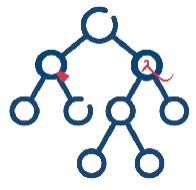
\includegraphics[height=1.0cm]{msca_logo.png}}%
    \end{center}

    \vspace{0.6cm}

    % Main title with Q logos on sides (with clickable links)
    \begin{center}
        \begin{minipage}{0.1\textwidth}
            \centering
            \href{https://quantlet.com}{
\includegraphics[height=1.1cm]{ql_logo.png}}
        \end{minipage}%
        \begin{minipage}{0.78\textwidth}
            \centering
            {\LARGE\bfseries\usebeamercolor[fg]{title}\inserttitle}

            \vspace{0.3cm}

            {\usebeamerfont{subtitle}\usebeamercolor[fg]{title}\insertsubtitle}
        \end{minipage}%
        \begin{minipage}{0.1\textwidth}
            \centering
            \href{https://quantinar.com}{
\includegraphics[height=1.1cm]{qr_logo.png}}
        \end{minipage}
    \end{center}

    \vspace{0.6cm}

    % Authors (left aligned)
    \hspace{0.5cm}{\usebeamerfont{author}\insertauthor}

    \vspace{0.3cm}

    % Institute/Affiliations (left aligned)
    \hspace{0.5cm}\begin{minipage}[t]{0.9\textwidth}
        \raggedright\small\insertinstitute
    \end{minipage}
}

%=============================================================================
% THEOREM ENVIRONMENTS
%=============================================================================
\theoremstyle{definition}
\setbeamertemplate{theorems}[numbered]
\ifdefined\atslang
\newtheorem{defn}{Definiție}
\newtheorem{thm}{Teoremă}
\newtheorem{prop}{Propoziție}
\newtheorem{rmk}{Observație}
\else
\newtheorem{defn}{Definition}
\newtheorem{thm}{Theorem}
\newtheorem{prop}{Proposition}
\newtheorem{rmk}{Remark}
\fi

%=============================================================================
% CENTRED MINIPAGE (no extra vertical space)
%=============================================================================
\newenvironment{cminipage}[1]{%
    \par\noindent\hfill\begin{minipage}{#1}\ignorespaces
}{%
    \end{minipage}\hfill\null\par
}

%=============================================================================
% CUSTOM COMMANDS
%=============================================================================
\newcommand{\E}{\mathbb{E}}
\newcommand{\Var}{\text{Var}}
\newcommand{\Cov}{\text{Cov}}
\newcommand{\Corr}{\text{Corr}}
\newcommand{\R}{\mathbb{R}}
\newcommand{\N}{\mathbb{N}}
\newcommand{\Z}{\mathbb{Z}}
\newcommand{\B}{\mathbf{B}}
\newcommand{\imark}{\textcolor{MainBlue}{\textbullet}}
\newcommand{\RMSE}{\text{RMSE}}
\newcommand{\MAE}{\text{MAE}}
\newcommand{\MAPE}{\text{MAPE}}

% Boldface vector/matrix commands (VAR, VECM, state space)
\newcommand{\bY}{\mathbf{Y}}
\newcommand{\bX}{\mathbf{X}}
\newcommand{\bA}{\mathbf{A}}
\newcommand{\bB}{\mathbf{B}}
\newcommand{\bepsilon}{\boldsymbol{\varepsilon}}
\newcommand{\bSigma}{\boldsymbol{\Sigma}}
\newcommand{\bPhi}{\boldsymbol{\Phi}}
\newcommand{\bGamma}{\boldsymbol{\Gamma}}
\newcommand{\bPi}{\boldsymbol{\Pi}}
\newcommand{\bc}{\mathbf{c}}
\newcommand{\balpha}{\boldsymbol{\alpha}}
\newcommand{\bbeta}{\boldsymbol{\beta}}
\newcommand{\bvarepsilon}{\boldsymbol{\varepsilon}}

% Seminar marks
\newcommand{\correct}{\textcolor{Forest}{\checkmark}}
\newcommand{\incorrect}{\textcolor{Crimson}{\texttimes}}
 se definește
%   \newcommand{\coursename}{Advanced Time Series Analysis and Forecasting}          (EN)
%   \newcommand{\coursename}{Analiza avansată a seriilor de timp și previziune}       (RO)  și  \def\atslang{ro}
% Fișierele .tex se află în EN/Courses, EN/Seminars, RO/Cursuri, RO/Seminarii (două niveluri sub rădăcină).
% Deck-urile sînt generate de latex/build_chapterN.py / build_seminarN.py (vezi latex/ats_build.py).

\documentclass[9pt, aspectratio=169, t]{beamer}
\providecommand{\coursename}{Advanced Time Series Analysis and Forecasting}

% Ensure content fits on slides
\setbeamersize{text margin left=8mm, text margin right=8mm}
% Smaller institute font (title page)
\setbeamerfont{institute}{size=\footnotesize}

%=============================================================================
% THEME AND STYLE CONFIGURATION
%=============================================================================
\usetheme{default}
% Using default theme for clean header/footer control

% Color Palette (matching Redispatch PDF)
\definecolor{MainBlue}{RGB}{26, 58, 110}
\definecolor{AccentBlue}{RGB}{26, 58, 110}
\definecolor{IDAred}{RGB}{205, 0, 0}
\definecolor{DarkGray}{RGB}{51, 51, 51}
\definecolor{MediumGray}{RGB}{128, 128, 128}
\definecolor{LightGray}{RGB}{248, 248, 248}
\definecolor{VeryLightGray}{RGB}{235, 235, 235}
\definecolor{KeynoteGray}{RGB}{218, 218, 218}
\definecolor{SectionGray}{RGB}{120, 120, 120}
\definecolor{FooterGray}{RGB}{100, 100, 100}
\definecolor{Crimson}{RGB}{220, 53, 69}
\definecolor{Forest}{RGB}{46, 125, 50}
\definecolor{Amber}{RGB}{181, 133, 63}
\definecolor{Orange}{RGB}{230, 126, 34}
\definecolor{Purple}{RGB}{142, 68, 173}

% Gradient background (exact Keynote 315° gradient: white to RGB 218,218,218)
\setbeamertemplate{background}{%
    \begin{tikzpicture}[remember picture, overlay]
        \shade[shading=axis, shading angle=315,
        top color=white, bottom color=KeynoteGray]
        (current page.south west) rectangle (current page.north east);
    \end{tikzpicture}%
}
% Fallback solid color for compatibility
\setbeamercolor{background canvas}{bg=}

\setbeamercolor{palette primary}{bg=MainBlue, fg=white}
\setbeamercolor{palette secondary}{bg=MainBlue!85, fg=white}
\setbeamercolor{palette tertiary}{bg=MainBlue!70, fg=white}
\setbeamercolor{structure}{fg=MainBlue}
\setbeamercolor{title}{fg=IDAred}
\setbeamercolor{frametitle}{fg=IDAred, bg=}
\setbeamercolor{block title}{bg=MainBlue, fg=white}
\setbeamercolor{block body}{bg=VeryLightGray, fg=DarkGray}
\setbeamercolor{block title alerted}{bg=Crimson, fg=white}
\setbeamercolor{block body alerted}{bg=Crimson!8, fg=DarkGray}
\setbeamercolor{block title example}{bg=Forest, fg=white}
\setbeamercolor{block body example}{bg=Forest!8, fg=DarkGray}
\setbeamercolor{item}{fg=MainBlue}

% Footer colors (override Madrid theme blue)
\setbeamercolor{author in head/foot}{fg=FooterGray, bg=}
\setbeamercolor{title in head/foot}{fg=FooterGray, bg=}
\setbeamercolor{date in head/foot}{fg=FooterGray, bg=}
\setbeamercolor{section in head/foot}{fg=FooterGray, bg=}
\setbeamercolor{subsection in head/foot}{fg=FooterGray, bg=}

% Bullet styles (apply everywhere including blocks)
\setbeamertemplate{itemize item}{\color{MainBlue}$\boxdot$}
\setbeamertemplate{itemize subitem}{\color{MainBlue}$\blacktriangleright$}
\setbeamertemplate{itemize subsubitem}{\color{MainBlue}\tiny$\bullet$}
\setbeamertemplate{itemize/enumerate body begin}{\normalsize}
\setbeamertemplate{itemize/enumerate subbody begin}{\normalsize}

% Item spacing - compact style
\setlength{\leftmargini}{10pt}       % Level 1: minimal indent
\setlength{\leftmarginii}{10pt}      % Level 2: minimal additional indent
% Compact list spacing (zero extra space before/after lists in blocks)
\makeatletter
\def\@listi{\leftmargin\leftmargini \topsep 0pt \parsep 0pt \itemsep 0pt}
\def\@listii{\leftmargin\leftmarginii \topsep 0pt \parsep 0pt \itemsep 0pt}
\makeatother

\setbeamertemplate{navigation symbols}{}

%=============================================================================
% CUSTOM HEADLINE
%=============================================================================
\setbeamertemplate{headline}{%
    \vskip10pt%
    \hbox to \paperwidth{%
        \hskip0.5cm%
        {\small\color{FooterGray}\renewcommand{\hyperlink}[2]{##2}\insertsectionhead}%
        \hfill%
        \textcolor{FooterGray}{\small\insertframenumber}%
        \hskip0.5cm%
    }%
    \vskip4pt%
    {\color{FooterGray}\hrule height 0.4pt}%
}

%=============================================================================
% CUSTOM FOOTER
%=============================================================================
\usepackage{fontawesome5}

\setbeamertemplate{footline}{%
    {\color{FooterGray}\hrule height 0.4pt}%
    \vskip4pt%
    \hbox to \paperwidth{%
        \hskip0.5cm%
        \textcolor{FooterGray}{\small\coursename}%
        \hfill%
        \raisebox{-0.1em}{%
            \begin{tikzpicture}[x=0.08em, y=0.08em, line width=0.4pt]
                \draw[FooterGray] (0,3) -- (1,4) -- (2,3.5) -- (3,5) -- (4,4) -- (5,6) -- (6,5.5) -- (7,4) -- (8,5) -- (9,7) -- (10,6) -- (11,5) -- (12,6.5) -- (13,8) -- (14,7) -- (15,6) -- (16,7.5) -- (17,9) -- (18,8) -- (19,7) -- (20,8.5) -- (21,10) -- (22,9) -- (23,8) -- (24,9.5);
            \end{tikzpicture}%
        }%
        \hskip0.5cm%
    }%
    \vskip6pt%
}

%=============================================================================
% PACKAGES
%=============================================================================
\usepackage[utf8]{inputenc}
\DeclareUnicodeCharacter{03B1}{\ensuremath{\alpha}}
\usepackage[T1]{fontenc}
\usepackage{amsmath, amssymb, amsthm}
\usepackage{mathtools}
\usepackage{bm}
\usepackage{tikz}
\usetikzlibrary{arrows.meta, positioning, shapes, calc, decorations.pathreplacing, shadings}
\usepackage{booktabs}
\usepackage{multirow}
\usepackage{array}
\usepackage{graphicx}
\usepackage{animate}
\usepackage{hyperref}
\usepackage{colortbl}
\usepackage{listings}
\lstset{language=Python, basicstyle=\ttfamily\scriptsize, keywordstyle=\color{MainBlue}\bfseries,
  commentstyle=\color{Forest}, stringstyle=\color{Crimson}, breaklines=true,
  frame=none, backgroundcolor=\color{VeryLightGray}, xleftmargin=2mm}
\hypersetup{colorlinks=true, linkcolor=MainBlue, urlcolor=MainBlue}
\graphicspath{{../../logos/}{../../charts/}{../../photos/}}
\usepackage{xcolor}
\hfuzz=2pt  % Suppress tiny overfull warnings (<2pt)
\vfuzz=2pt  % Suppress tiny vertical overfull warnings (<2pt)

%=============================================================================
% QUANTLET COMMANDS
%   \quantlet{<displayed name>}{<url>}       (generic)
%   \atsquantlet{Ch_05}{ATS_ch5_garch}       -> https://github.com/danpele/Advanced-Time-Series/tree/main/Quantlets/Ch_05/ATS_ch5_garch
%   \qlurl{<folder>} is defined per chapter by the generator (Quantlets/Ch_NN/<folder>)
%=============================================================================
\newcommand{\atsrepo}{https://github.com/danpele/Advanced-Time-Series}
\newcommand{\atsqlbase}{https://github.com/danpele/Advanced-Time-Series/tree/main/Quantlets}
\newcommand{\quantlet}[2]{%
    \hfill\href{#2}{%
        \raisebox{-0.15em}{
\includegraphics[height=0.7em]{ql_logo.png}}%
        \textcolor{MainBlue}{\tiny\ #1}%
    }%
}
\newcommand{\atsquantlet}[2]{\quantlet{\detokenize{#2}}{\atsqlbase/#1/#2}}

%=============================================================================
% NOTEBOOKS (Google Colab)
%   \colaburl{notebooks/EN/chapter5_seminar_notebook.ipynb} -> the Colab link of a file in the ATS repo
%   \nb: the chapter notebook (each seminar deck redefines it with \renewcommand)
%=============================================================================
\newcommand{\colaburl}[1]{https://colab.research.google.com/github/danpele/Advanced-Time-Series/blob/main/#1}
\newcommand{\nb}{https://colab.research.google.com/github/danpele/Advanced-Time-Series/tree/main/notebooks/EN}
\newcommand{\nbname}{notebooks/EN}

%=============================================================================
% SLIDE HELPERS (used by the generators; the same as in MFM)
%=============================================================================
% local font size for list bodies (the preamble forces \normalsize)
\newcommand{\itemsize}[1]{\setbeamertemplate{itemize/enumerate body begin}{#1}\setbeamertemplate{itemize/enumerate subbody begin}{#1}}
\newcommand{\intitle}[1]{{\hypersetup{urlcolor=white}#1}}   % white links inside coloured title bars
\newcommand{\imgcap}[1]{{\scriptsize #1}\\[0.5mm]}          % caption under a photo
\newcommand{\imgcredit}[2]{{\tiny\color{FooterGray}\href{#1}{#2}}}   % image credit: source URL, author/licence
\newcommand{\aiprompt}[1]{{\ttfamily\color{MainBlue}#1}}     % a prompt to an AI assistant

%=============================================================================
% SEMINARS: student version by default; the instructor wrapper *_solutions.tex sets \solutionstrue
%=============================================================================
\makeatletter\@ifundefined{ifsolutions}{\expandafter\newif\csname ifsolutions\endcsname}{}\makeatother
\newcommand{\solonly}[1]{\ifsolutions #1\fi}
\newcommand{\propsub}{\ifsolutions\else\framesubtitle{\ifdefined\atslang Rezolvarea se discută la seminar\else Solution discussed in class\fi}\fi}

%=============================================================================
% APPENDIX AND CHAPTER LINKS (latex/appendix_links.py writes the calls; it also re-declares these
% macros before \begin{document}, so the decks compile with or without this preamble block)
%=============================================================================
\providecommand{\atsapplink}[3]{\hypertarget{#2}{}\hyperlink{#1}{\beamergotobutton{#3}}}
\providecommand{\atsappback}[2]{\begin{tikzpicture}[remember picture,overlay]\node[anchor=south east] at ([xshift=-3mm,yshift=7mm]current page.south east){\hyperlink{#1}{\beamerreturnbutton{#2}}};\end{tikzpicture}}
\providecommand{\atschlink}[2]{\href{#1}{#2}}
\providecommand{\atschlinkt}[2]{\href{#1}{\usebeamercolor[fg]{frametitle}#2}}

%=============================================================================
% QUANTINAR COMMAND: link către un curs Quantinar (subiecte avansate)
%=============================================================================
\newcommand{\quantinar}[2]{%
    \href{#2}{%
        \raisebox{-0.15em}{
\includegraphics[height=0.8em]{qr_logo.png}}%
        \textcolor{MainBlue}{\scriptsize\ #1}%
    }%
}

%=============================================================================
% CUSTOM TITLE PAGE
%=============================================================================
\defbeamertemplate*{title page}{hybrid}[1][]
{
    \vspace{0.2cm}
    % Logos row - top header (with clickable links)
    \begin{center}
        \href{https://www.ase.ro}{
\includegraphics[height=1.0cm]{ase_logo.png}}\hspace{0.3cm}%
        \href{https://theida.net}{
\includegraphics[height=1.0cm]{ida_logo.png}}\hspace{0.3cm}%
        \href{https://blockchain-research-center.com}{
\includegraphics[height=1.0cm]{brc_logo.png}}\hspace{0.3cm}%
        \href{https://www.ai4efin.ase.ro}{
\includegraphics[height=1.0cm]{ai4efin_logo.png}}\hspace{0.3cm}%
        \href{https://ipe.ro/new}{
\includegraphics[height=1.0cm]{acad_logo.png}}\hspace{0.3cm}%
        \href{https://www.digital-finance-msca.com}{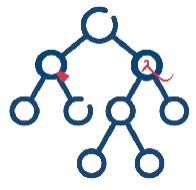
\includegraphics[height=1.0cm]{msca_logo.png}}%
    \end{center}

    \vspace{0.6cm}

    % Main title with Q logos on sides (with clickable links)
    \begin{center}
        \begin{minipage}{0.1\textwidth}
            \centering
            \href{https://quantlet.com}{
\includegraphics[height=1.1cm]{ql_logo.png}}
        \end{minipage}%
        \begin{minipage}{0.78\textwidth}
            \centering
            {\LARGE\bfseries\usebeamercolor[fg]{title}\inserttitle}

            \vspace{0.3cm}

            {\usebeamerfont{subtitle}\usebeamercolor[fg]{title}\insertsubtitle}
        \end{minipage}%
        \begin{minipage}{0.1\textwidth}
            \centering
            \href{https://quantinar.com}{
\includegraphics[height=1.1cm]{qr_logo.png}}
        \end{minipage}
    \end{center}

    \vspace{0.6cm}

    % Authors (left aligned)
    \hspace{0.5cm}{\usebeamerfont{author}\insertauthor}

    \vspace{0.3cm}

    % Institute/Affiliations (left aligned)
    \hspace{0.5cm}\begin{minipage}[t]{0.9\textwidth}
        \raggedright\small\insertinstitute
    \end{minipage}
}

%=============================================================================
% THEOREM ENVIRONMENTS
%=============================================================================
\theoremstyle{definition}
\setbeamertemplate{theorems}[numbered]
\ifdefined\atslang
\newtheorem{defn}{Definiție}
\newtheorem{thm}{Teoremă}
\newtheorem{prop}{Propoziție}
\newtheorem{rmk}{Observație}
\else
\newtheorem{defn}{Definition}
\newtheorem{thm}{Theorem}
\newtheorem{prop}{Proposition}
\newtheorem{rmk}{Remark}
\fi

%=============================================================================
% CENTRED MINIPAGE (no extra vertical space)
%=============================================================================
\newenvironment{cminipage}[1]{%
    \par\noindent\hfill\begin{minipage}{#1}\ignorespaces
}{%
    \end{minipage}\hfill\null\par
}

%=============================================================================
% CUSTOM COMMANDS
%=============================================================================
\newcommand{\E}{\mathbb{E}}
\newcommand{\Var}{\text{Var}}
\newcommand{\Cov}{\text{Cov}}
\newcommand{\Corr}{\text{Corr}}
\newcommand{\R}{\mathbb{R}}
\newcommand{\N}{\mathbb{N}}
\newcommand{\Z}{\mathbb{Z}}
\newcommand{\B}{\mathbf{B}}
\newcommand{\imark}{\textcolor{MainBlue}{\textbullet}}
\newcommand{\RMSE}{\text{RMSE}}
\newcommand{\MAE}{\text{MAE}}
\newcommand{\MAPE}{\text{MAPE}}

% Boldface vector/matrix commands (VAR, VECM, state space)
\newcommand{\bY}{\mathbf{Y}}
\newcommand{\bX}{\mathbf{X}}
\newcommand{\bA}{\mathbf{A}}
\newcommand{\bB}{\mathbf{B}}
\newcommand{\bepsilon}{\boldsymbol{\varepsilon}}
\newcommand{\bSigma}{\boldsymbol{\Sigma}}
\newcommand{\bPhi}{\boldsymbol{\Phi}}
\newcommand{\bGamma}{\boldsymbol{\Gamma}}
\newcommand{\bPi}{\boldsymbol{\Pi}}
\newcommand{\bc}{\mathbf{c}}
\newcommand{\balpha}{\boldsymbol{\alpha}}
\newcommand{\bbeta}{\boldsymbol{\beta}}
\newcommand{\bvarepsilon}{\boldsymbol{\varepsilon}}

% Seminar marks
\newcommand{\correct}{\textcolor{Forest}{\checkmark}}
\newcommand{\incorrect}{\textcolor{Crimson}{\texttimes}}
 se definește
%   \newcommand{\coursename}{Advanced Time Series Analysis and Forecasting}          (EN)
%   \newcommand{\coursename}{Analiza avansată a seriilor de timp și previziune}       (RO)  și  \def\atslang{ro}
% Fișierele .tex se află în EN/Courses, EN/Seminars, RO/Cursuri, RO/Seminarii (două niveluri sub rădăcină).
% Deck-urile sînt generate de latex/build_chapterN.py / build_seminarN.py (vezi latex/ats_build.py).

\documentclass[9pt, aspectratio=169, t]{beamer}
\providecommand{\coursename}{Advanced Time Series Analysis and Forecasting}

% Ensure content fits on slides
\setbeamersize{text margin left=8mm, text margin right=8mm}
% Smaller institute font (title page)
\setbeamerfont{institute}{size=\footnotesize}

%=============================================================================
% THEME AND STYLE CONFIGURATION
%=============================================================================
\usetheme{default}
% Using default theme for clean header/footer control

% Color Palette (matching Redispatch PDF)
\definecolor{MainBlue}{RGB}{26, 58, 110}
\definecolor{AccentBlue}{RGB}{26, 58, 110}
\definecolor{IDAred}{RGB}{205, 0, 0}
\definecolor{DarkGray}{RGB}{51, 51, 51}
\definecolor{MediumGray}{RGB}{128, 128, 128}
\definecolor{LightGray}{RGB}{248, 248, 248}
\definecolor{VeryLightGray}{RGB}{235, 235, 235}
\definecolor{KeynoteGray}{RGB}{218, 218, 218}
\definecolor{SectionGray}{RGB}{120, 120, 120}
\definecolor{FooterGray}{RGB}{100, 100, 100}
\definecolor{Crimson}{RGB}{220, 53, 69}
\definecolor{Forest}{RGB}{46, 125, 50}
\definecolor{Amber}{RGB}{181, 133, 63}
\definecolor{Orange}{RGB}{230, 126, 34}
\definecolor{Purple}{RGB}{142, 68, 173}

% Gradient background (exact Keynote 315° gradient: white to RGB 218,218,218)
\setbeamertemplate{background}{%
    \begin{tikzpicture}[remember picture, overlay]
        \shade[shading=axis, shading angle=315,
        top color=white, bottom color=KeynoteGray]
        (current page.south west) rectangle (current page.north east);
    \end{tikzpicture}%
}
% Fallback solid color for compatibility
\setbeamercolor{background canvas}{bg=}

\setbeamercolor{palette primary}{bg=MainBlue, fg=white}
\setbeamercolor{palette secondary}{bg=MainBlue!85, fg=white}
\setbeamercolor{palette tertiary}{bg=MainBlue!70, fg=white}
\setbeamercolor{structure}{fg=MainBlue}
\setbeamercolor{title}{fg=IDAred}
\setbeamercolor{frametitle}{fg=IDAred, bg=}
\setbeamercolor{block title}{bg=MainBlue, fg=white}
\setbeamercolor{block body}{bg=VeryLightGray, fg=DarkGray}
\setbeamercolor{block title alerted}{bg=Crimson, fg=white}
\setbeamercolor{block body alerted}{bg=Crimson!8, fg=DarkGray}
\setbeamercolor{block title example}{bg=Forest, fg=white}
\setbeamercolor{block body example}{bg=Forest!8, fg=DarkGray}
\setbeamercolor{item}{fg=MainBlue}

% Footer colors (override Madrid theme blue)
\setbeamercolor{author in head/foot}{fg=FooterGray, bg=}
\setbeamercolor{title in head/foot}{fg=FooterGray, bg=}
\setbeamercolor{date in head/foot}{fg=FooterGray, bg=}
\setbeamercolor{section in head/foot}{fg=FooterGray, bg=}
\setbeamercolor{subsection in head/foot}{fg=FooterGray, bg=}

% Bullet styles (apply everywhere including blocks)
\setbeamertemplate{itemize item}{\color{MainBlue}$\boxdot$}
\setbeamertemplate{itemize subitem}{\color{MainBlue}$\blacktriangleright$}
\setbeamertemplate{itemize subsubitem}{\color{MainBlue}\tiny$\bullet$}
\setbeamertemplate{itemize/enumerate body begin}{\normalsize}
\setbeamertemplate{itemize/enumerate subbody begin}{\normalsize}

% Item spacing - compact style
\setlength{\leftmargini}{10pt}       % Level 1: minimal indent
\setlength{\leftmarginii}{10pt}      % Level 2: minimal additional indent
% Compact list spacing (zero extra space before/after lists in blocks)
\makeatletter
\def\@listi{\leftmargin\leftmargini \topsep 0pt \parsep 0pt \itemsep 0pt}
\def\@listii{\leftmargin\leftmarginii \topsep 0pt \parsep 0pt \itemsep 0pt}
\makeatother

\setbeamertemplate{navigation symbols}{}

%=============================================================================
% CUSTOM HEADLINE
%=============================================================================
\setbeamertemplate{headline}{%
    \vskip10pt%
    \hbox to \paperwidth{%
        \hskip0.5cm%
        {\small\color{FooterGray}\renewcommand{\hyperlink}[2]{##2}\insertsectionhead}%
        \hfill%
        \textcolor{FooterGray}{\small\insertframenumber}%
        \hskip0.5cm%
    }%
    \vskip4pt%
    {\color{FooterGray}\hrule height 0.4pt}%
}

%=============================================================================
% CUSTOM FOOTER
%=============================================================================
\usepackage{fontawesome5}

\setbeamertemplate{footline}{%
    {\color{FooterGray}\hrule height 0.4pt}%
    \vskip4pt%
    \hbox to \paperwidth{%
        \hskip0.5cm%
        \textcolor{FooterGray}{\small\coursename}%
        \hfill%
        \raisebox{-0.1em}{%
            \begin{tikzpicture}[x=0.08em, y=0.08em, line width=0.4pt]
                \draw[FooterGray] (0,3) -- (1,4) -- (2,3.5) -- (3,5) -- (4,4) -- (5,6) -- (6,5.5) -- (7,4) -- (8,5) -- (9,7) -- (10,6) -- (11,5) -- (12,6.5) -- (13,8) -- (14,7) -- (15,6) -- (16,7.5) -- (17,9) -- (18,8) -- (19,7) -- (20,8.5) -- (21,10) -- (22,9) -- (23,8) -- (24,9.5);
            \end{tikzpicture}%
        }%
        \hskip0.5cm%
    }%
    \vskip6pt%
}

%=============================================================================
% PACKAGES
%=============================================================================
\usepackage[utf8]{inputenc}
\DeclareUnicodeCharacter{03B1}{\ensuremath{\alpha}}
\usepackage[T1]{fontenc}
\usepackage{amsmath, amssymb, amsthm}
\usepackage{mathtools}
\usepackage{bm}
\usepackage{tikz}
\usetikzlibrary{arrows.meta, positioning, shapes, calc, decorations.pathreplacing, shadings}
\usepackage{booktabs}
\usepackage{multirow}
\usepackage{array}
\usepackage{graphicx}
\usepackage{animate}
\usepackage{hyperref}
\usepackage{colortbl}
\usepackage{listings}
\lstset{language=Python, basicstyle=\ttfamily\scriptsize, keywordstyle=\color{MainBlue}\bfseries,
  commentstyle=\color{Forest}, stringstyle=\color{Crimson}, breaklines=true,
  frame=none, backgroundcolor=\color{VeryLightGray}, xleftmargin=2mm}
\hypersetup{colorlinks=true, linkcolor=MainBlue, urlcolor=MainBlue}
\graphicspath{{../../logos/}{../../charts/}{../../photos/}}
\usepackage{xcolor}
\hfuzz=2pt  % Suppress tiny overfull warnings (<2pt)
\vfuzz=2pt  % Suppress tiny vertical overfull warnings (<2pt)

%=============================================================================
% QUANTLET COMMANDS
%   \quantlet{<displayed name>}{<url>}       (generic)
%   \atsquantlet{Ch_05}{ATS_ch5_garch}       -> https://github.com/danpele/Advanced-Time-Series/tree/main/Quantlets/Ch_05/ATS_ch5_garch
%   \qlurl{<folder>} is defined per chapter by the generator (Quantlets/Ch_NN/<folder>)
%=============================================================================
\newcommand{\atsrepo}{https://github.com/danpele/Advanced-Time-Series}
\newcommand{\atsqlbase}{https://github.com/danpele/Advanced-Time-Series/tree/main/Quantlets}
\newcommand{\quantlet}[2]{%
    \hfill\href{#2}{%
        \raisebox{-0.15em}{
\includegraphics[height=0.7em]{ql_logo.png}}%
        \textcolor{MainBlue}{\tiny\ #1}%
    }%
}
\newcommand{\atsquantlet}[2]{\quantlet{\detokenize{#2}}{\atsqlbase/#1/#2}}

%=============================================================================
% NOTEBOOKS (Google Colab)
%   \colaburl{notebooks/EN/chapter5_seminar_notebook.ipynb} -> the Colab link of a file in the ATS repo
%   \nb: the chapter notebook (each seminar deck redefines it with \renewcommand)
%=============================================================================
\newcommand{\colaburl}[1]{https://colab.research.google.com/github/danpele/Advanced-Time-Series/blob/main/#1}
\newcommand{\nb}{https://colab.research.google.com/github/danpele/Advanced-Time-Series/tree/main/notebooks/EN}
\newcommand{\nbname}{notebooks/EN}

%=============================================================================
% SLIDE HELPERS (used by the generators; the same as in MFM)
%=============================================================================
% local font size for list bodies (the preamble forces \normalsize)
\newcommand{\itemsize}[1]{\setbeamertemplate{itemize/enumerate body begin}{#1}\setbeamertemplate{itemize/enumerate subbody begin}{#1}}
\newcommand{\intitle}[1]{{\hypersetup{urlcolor=white}#1}}   % white links inside coloured title bars
\newcommand{\imgcap}[1]{{\scriptsize #1}\\[0.5mm]}          % caption under a photo
\newcommand{\imgcredit}[2]{{\tiny\color{FooterGray}\href{#1}{#2}}}   % image credit: source URL, author/licence
\newcommand{\aiprompt}[1]{{\ttfamily\color{MainBlue}#1}}     % a prompt to an AI assistant

%=============================================================================
% SEMINARS: student version by default; the instructor wrapper *_solutions.tex sets \solutionstrue
%=============================================================================
\makeatletter\@ifundefined{ifsolutions}{\expandafter\newif\csname ifsolutions\endcsname}{}\makeatother
\newcommand{\solonly}[1]{\ifsolutions #1\fi}
\newcommand{\propsub}{\ifsolutions\else\framesubtitle{\ifdefined\atslang Rezolvarea se discută la seminar\else Solution discussed in class\fi}\fi}

%=============================================================================
% APPENDIX AND CHAPTER LINKS (latex/appendix_links.py writes the calls; it also re-declares these
% macros before \begin{document}, so the decks compile with or without this preamble block)
%=============================================================================
\providecommand{\atsapplink}[3]{\hypertarget{#2}{}\hyperlink{#1}{\beamergotobutton{#3}}}
\providecommand{\atsappback}[2]{\begin{tikzpicture}[remember picture,overlay]\node[anchor=south east] at ([xshift=-3mm,yshift=7mm]current page.south east){\hyperlink{#1}{\beamerreturnbutton{#2}}};\end{tikzpicture}}
\providecommand{\atschlink}[2]{\href{#1}{#2}}
\providecommand{\atschlinkt}[2]{\href{#1}{\usebeamercolor[fg]{frametitle}#2}}

%=============================================================================
% QUANTINAR COMMAND: link către un curs Quantinar (subiecte avansate)
%=============================================================================
\newcommand{\quantinar}[2]{%
    \href{#2}{%
        \raisebox{-0.15em}{
\includegraphics[height=0.8em]{qr_logo.png}}%
        \textcolor{MainBlue}{\scriptsize\ #1}%
    }%
}

%=============================================================================
% CUSTOM TITLE PAGE
%=============================================================================
\defbeamertemplate*{title page}{hybrid}[1][]
{
    \vspace{0.2cm}
    % Logos row - top header (with clickable links)
    \begin{center}
        \href{https://www.ase.ro}{
\includegraphics[height=1.0cm]{ase_logo.png}}\hspace{0.3cm}%
        \href{https://theida.net}{
\includegraphics[height=1.0cm]{ida_logo.png}}\hspace{0.3cm}%
        \href{https://blockchain-research-center.com}{
\includegraphics[height=1.0cm]{brc_logo.png}}\hspace{0.3cm}%
        \href{https://www.ai4efin.ase.ro}{
\includegraphics[height=1.0cm]{ai4efin_logo.png}}\hspace{0.3cm}%
        \href{https://ipe.ro/new}{
\includegraphics[height=1.0cm]{acad_logo.png}}\hspace{0.3cm}%
        \href{https://www.digital-finance-msca.com}{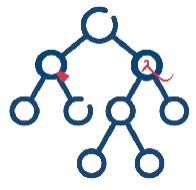
\includegraphics[height=1.0cm]{msca_logo.png}}%
    \end{center}

    \vspace{0.6cm}

    % Main title with Q logos on sides (with clickable links)
    \begin{center}
        \begin{minipage}{0.1\textwidth}
            \centering
            \href{https://quantlet.com}{
\includegraphics[height=1.1cm]{ql_logo.png}}
        \end{minipage}%
        \begin{minipage}{0.78\textwidth}
            \centering
            {\LARGE\bfseries\usebeamercolor[fg]{title}\inserttitle}

            \vspace{0.3cm}

            {\usebeamerfont{subtitle}\usebeamercolor[fg]{title}\insertsubtitle}
        \end{minipage}%
        \begin{minipage}{0.1\textwidth}
            \centering
            \href{https://quantinar.com}{
\includegraphics[height=1.1cm]{qr_logo.png}}
        \end{minipage}
    \end{center}

    \vspace{0.6cm}

    % Authors (left aligned)
    \hspace{0.5cm}{\usebeamerfont{author}\insertauthor}

    \vspace{0.3cm}

    % Institute/Affiliations (left aligned)
    \hspace{0.5cm}\begin{minipage}[t]{0.9\textwidth}
        \raggedright\small\insertinstitute
    \end{minipage}
}

%=============================================================================
% THEOREM ENVIRONMENTS
%=============================================================================
\theoremstyle{definition}
\setbeamertemplate{theorems}[numbered]
\ifdefined\atslang
\newtheorem{defn}{Definiție}
\newtheorem{thm}{Teoremă}
\newtheorem{prop}{Propoziție}
\newtheorem{rmk}{Observație}
\else
\newtheorem{defn}{Definition}
\newtheorem{thm}{Theorem}
\newtheorem{prop}{Proposition}
\newtheorem{rmk}{Remark}
\fi

%=============================================================================
% CENTRED MINIPAGE (no extra vertical space)
%=============================================================================
\newenvironment{cminipage}[1]{%
    \par\noindent\hfill\begin{minipage}{#1}\ignorespaces
}{%
    \end{minipage}\hfill\null\par
}

%=============================================================================
% CUSTOM COMMANDS
%=============================================================================
\newcommand{\E}{\mathbb{E}}
\newcommand{\Var}{\text{Var}}
\newcommand{\Cov}{\text{Cov}}
\newcommand{\Corr}{\text{Corr}}
\newcommand{\R}{\mathbb{R}}
\newcommand{\N}{\mathbb{N}}
\newcommand{\Z}{\mathbb{Z}}
\newcommand{\B}{\mathbf{B}}
\newcommand{\imark}{\textcolor{MainBlue}{\textbullet}}
\newcommand{\RMSE}{\text{RMSE}}
\newcommand{\MAE}{\text{MAE}}
\newcommand{\MAPE}{\text{MAPE}}

% Boldface vector/matrix commands (VAR, VECM, state space)
\newcommand{\bY}{\mathbf{Y}}
\newcommand{\bX}{\mathbf{X}}
\newcommand{\bA}{\mathbf{A}}
\newcommand{\bB}{\mathbf{B}}
\newcommand{\bepsilon}{\boldsymbol{\varepsilon}}
\newcommand{\bSigma}{\boldsymbol{\Sigma}}
\newcommand{\bPhi}{\boldsymbol{\Phi}}
\newcommand{\bGamma}{\boldsymbol{\Gamma}}
\newcommand{\bPi}{\boldsymbol{\Pi}}
\newcommand{\bc}{\mathbf{c}}
\newcommand{\balpha}{\boldsymbol{\alpha}}
\newcommand{\bbeta}{\boldsymbol{\beta}}
\newcommand{\bvarepsilon}{\boldsymbol{\varepsilon}}

% Seminar marks
\newcommand{\correct}{\textcolor{Forest}{\checkmark}}
\newcommand{\incorrect}{\textcolor{Crimson}{\texttimes}}


\newcommand{\qlurl}[1]{https://github.com/danpele/Advanced-Time-Series/tree/main/Quantlets/Ch_12/#1}

% Clickable citations (DOIs verified via Crossref)
\newcommand{\refBaiK}{\href{https://arxiv.org/abs/1803.01271}{Bai, Kolter and Koltun (2018)}}
\newcommand{\refBCH}{\href{https://doi.org/10.1093/restud/rdt044}{Belloni, Chernozhukov and Hansen (2014)}}
\newcommand{\refBSF}{\href{https://doi.org/10.1109/72.279181}{Bengio, Simard and Frasconi (1994)}}
\newcommand{\refBen}{\href{https://doi.org/10.1145/3533382}{Benidis et al.\ (2022)}}
\newcommand{\refBB}{\href{https://doi.org/10.1016/j.ins.2011.12.028}{Bergmeir and Benítez (2012)}}
\newcommand{\refBHK}{\href{https://doi.org/10.1016/j.csda.2017.11.003}{Bergmeir, Hyndman and Koo (2018)}}
\newcommand{\refBerk}{\href{https://doi.org/10.1214/12-AOS1077}{Berk et al.\ (2013)}}
\newcommand{\refBM}{\href{https://doi.org/10.1214/15-AOS1315}{Basu and Michailidis (2015)}}
\newcommand{\refBreA}{\href{https://doi.org/10.1007/BF00058655}{Breiman (1996)}}
\newcommand{\refBreB}{\href{https://doi.org/10.1023/A:1010933404324}{Breiman (2001)}}
\newcommand{\refBuc}{\href{https://doi.org/10.1093/jjfinec/nbaa008}{Bucci (2020)}}
\newcommand{\refBCN}{\href{https://doi.org/10.1093/biomet/81.2.351}{Burman, Chow and Nolan (1994)}}
\newcommand{\refNHiTS}{\href{https://doi.org/10.1609/aaai.v37i6.25854}{Challu et al.\ (2023)}}
\newcommand{\refCG}{\href{https://doi.org/10.1145/2939672.2939785}{Chen and Guestrin (2016)}}
\newcommand{\refCho}{\href{https://doi.org/10.3115/v1/D14-1179}{Cho et al.\ (2014)}}
\newcommand{\refCSV}{\href{https://doi.org/10.1093/jjfinec/nbac020}{Christensen, Siggaard and Veliyev (2023)}}
\newcommand{\refCor}{\href{https://doi.org/10.1093/jjfinec/nbp001}{Corsi (2009)}}
\newcommand{\refDM}{\href{https://doi.org/10.1080/07350015.1995.10524599}{Diebold and Mariano (1995)}}
\newcommand{\refFri}{\href{https://doi.org/10.1214/aos/1013203451}{Friedman (2001)}}
\newcommand{\refGSC}{\href{https://doi.org/10.1162/089976600300015015}{Gers, Schmidhuber and Cummins (2000)}}
\newcommand{\refGR}{\href{https://doi.org/10.1198/016214506000001437}{Gneiting and Raftery (2007)}}
\newcommand{\refGCLSS}{\href{https://doi.org/10.1002/jae.2910}{Goulet Coulombe et al.\ (2022)}}
\newcommand{\refGKX}{\href{https://doi.org/10.1093/rfs/hhaa009}{Gu, Kelly and Xiu (2020)}}
\newcommand{\refHan}{\href{https://doi.org/10.1198/073500105000000063}{Hansen (2005)}}
\newcommand{\refHLN}{\href{https://doi.org/10.3982/ECTA5771}{Hansen, Lunde and Nason (2011)}}
\newcommand{\refOMI}{\href{https://web.archive.org/web/20220301022212/https://realized.oxford-man.ox.ac.uk/}{Heber et al.\ (2009)}}
\newcommand{\refHAB}{\href{https://doi.org/10.1007/s10618-022-00894-5}{Hewamalage, Ackermann and Bergmeir (2023)}}
\newcommand{\refHBB}{\href{https://doi.org/10.1016/j.ijforecast.2020.06.008}{Hewamalage, Bergmeir and Bandara (2021)}}
\newcommand{\refHS}{\href{https://doi.org/10.1162/neco.1997.9.8.1735}{Hochreiter and Schmidhuber (1997)}}
\newcommand{\refHK}{\href{https://doi.org/10.1016/j.ijforecast.2006.03.001}{Hyndman and Koehler (2006)}}
\newcommand{\refJW}{\href{https://doi.org/10.18653/v1/N19-1357}{Jain and Wallace (2019)}}
\newcommand{\refJZS}{\href{https://proceedings.mlr.press/v37/jozefowicz15.html}{Jozefowicz, Zaremba and Sutskever (2015)}}
\newcommand{\refKeA}{\href{https://proceedings.neurips.cc/paper/2017/hash/6449f44a102fde848669bdd9eb6b76fa-Abstract.html}{Ke et al.\ (2017)}}
\newcommand{\refKB}{\href{https://arxiv.org/abs/1412.6980}{Kingma and Ba (2015)}}
\newcommand{\refLMDW}{\href{https://doi.org/10.1016/j.apenergy.2021.116983}{Lago et al.\ (2021)}}
\newcommand{\refLSST}{\href{https://doi.org/10.1214/15-AOS1371}{Lee et al.\ (2016)}}
\newcommand{\refTFT}{\href{https://doi.org/10.1016/j.ijforecast.2021.03.012}{Lim et al.\ (2021)}}
\newcommand{\refLL}{\href{https://proceedings.neurips.cc/paper/2017/hash/8a20a8621978632d76c43dfd28b67767-Abstract.html}{Lundberg and Lee (2017)}}
\newcommand{\refMSAa}{\href{https://doi.org/10.1371/journal.pone.0194889}{Makridakis, Spiliotis and Assimakopoulos (2018)}}
\newcommand{\refMfourA}{\href{https://doi.org/10.1016/j.ijforecast.2019.04.014}{Makridakis, Spiliotis and Assimakopoulos (2020)}}
\newcommand{\refMfiveA}{\href{https://doi.org/10.1016/j.ijforecast.2021.11.013}{Makridakis, Spiliotis and Assimakopoulos (2022)}}
\newcommand{\refMM}{\href{https://doi.org/10.1016/j.jeconom.2015.10.011}{Medeiros and Mendes (2016)}}
\newcommand{\refMVVZ}{\href{https://doi.org/10.1080/07350015.2019.1637745}{Medeiros et al.\ (2021)}}
\newcommand{\refMei}{\href{https://jmlr.org/papers/v7/meinshausen06a.html}{Meinshausen (2006)}}
\newcommand{\refMR}{\href{https://jmlr.org/papers/v11/mohri10a.html}{Mohri and Rostamizadeh (2010)}}
\newcommand{\refMMH}{\href{https://doi.org/10.1016/j.ijforecast.2021.03.004}{Montero-Manso and Hyndman (2021)}}
\newcommand{\refNie}{\href{https://arxiv.org/abs/2211.14730}{Nie et al.\ (2023)}}
\newcommand{\refOre}{\href{https://arxiv.org/abs/1905.10437}{Oreshkin et al.\ (2020)}}
\newcommand{\refPMB}{\href{https://proceedings.mlr.press/v28/pascanu13.html}{Pascanu, Mikolov and Bengio (2013)}}
\newcommand{\refPat}{\href{https://doi.org/10.1016/j.jeconom.2010.03.034}{Patton (2011)}}
\newcommand{\refPet}{\href{https://doi.org/10.1016/j.ijforecast.2021.11.001}{Petropoulos et al.\ (2022)}}
\newcommand{\refRac}{\href{https://doi.org/10.1016/S0304-4076(00)00030-0}{Racine (2000)}}
\newcommand{\refRHW}{\href{https://doi.org/10.1038/323533a0}{Rumelhart, Hinton and Williams (1986)}}
\newcommand{\refDeepAR}{\href{https://doi.org/10.1016/j.ijforecast.2019.07.001}{Salinas et al.\ (2020)}}
\newcommand{\refSBV}{\href{https://doi.org/10.1214/15-AOS1321}{Scornet, Biau and Vert (2015)}}
\newcommand{\refSha}{\href{https://doi.org/10.1515/9781400881970-018}{Shapley (1953)}}
\newcommand{\refSmyl}{\href{https://doi.org/10.1016/j.ijforecast.2019.03.017}{Smyl (2020)}}
\newcommand{\refSVL}{\href{https://arxiv.org/abs/1409.3215}{Sutskever, Vinyals and Le (2014)}}
\newcommand{\refTib}{\href{https://doi.org/10.1111/j.2517-6161.1996.tb02080.x}{Tibshirani (1996)}}
\newcommand{\refWaveNet}{\href{https://arxiv.org/abs/1609.03499}{van den Oord et al.\ (2016)}}
\newcommand{\refVas}{\href{https://proceedings.neurips.cc/paper/2017/hash/3f5ee243547dee91fbd053c1c4a845aa-Abstract.html}{Vaswani et al.\ (2017)}}
\newcommand{\refWA}{\href{https://doi.org/10.1080/01621459.2017.1319839}{Wager and Athey (2018)}}
\newcommand{\refWhi}{\href{https://doi.org/10.1111/1468-0262.00152}{White (2000)}}
\newcommand{\refWP}{\href{https://doi.org/10.18653/v1/D19-1002}{Wiegreffe and Pinter (2019)}}
\newcommand{\refAuto}{\href{https://proceedings.neurips.cc/paper/2021/hash/bcc0d400288793e8bdcd7c19a8ac0c2b-Abstract.html}{Wu et al.\ (2021)}}
\newcommand{\refYu}{\href{https://doi.org/10.1214/aop/1176988849}{Yu (1994)}}
\newcommand{\refZeng}{\href{https://doi.org/10.1609/aaai.v37i9.26317}{Zeng et al.\ (2023)}}
\newcommand{\refZY}{\href{https://jmlr.org/papers/v7/zhao06a.html}{Zhao and Yu (2006)}}
\newcommand{\refInf}{\href{https://doi.org/10.1609/aaai.v35i12.17325}{Zhou et al.\ (2021)}}
\newcommand{\refZW}{\href{https://doi.org/10.1016/j.eneco.2017.12.016}{Ziel and Weron (2018)}}
\newcommand{\refZou}{\href{https://doi.org/10.1198/016214506000000735}{Zou (2006)}}
\newcommand{\refZH}{\href{https://doi.org/10.1111/j.1467-9868.2005.00503.x}{Zou and Hastie (2005)}}

\title[Advanced Time Series Analysis and Forecasting]{Advanced Time Series Analysis and Forecasting}
\subtitle{Chapter 12: Machine learning and deep learning for time series}
\author[D.T. Pele]{Daniel Traian PELE}
\institute{Bucharest University of Economic Studies\\
IDA Institute Digital Assets\\
Blockchain Research Center\\
AI4EFin Artificial Intelligence for Energy Finance\\
Romanian Academy, Institute for Economic Forecasting\\
MSCA Digital Finance}
\date{}

%=============================================================================
\providecommand{\atsapplink}[3]{\hypertarget{#2}{}\hyperlink{#1}{\beamergotobutton{#3}}}  % APPLINKS-MACROS
\providecommand{\atsappback}[2]{\begin{tikzpicture}[remember picture,overlay]\node[anchor=south east] at ([xshift=-3mm,yshift=7mm]current page.south east){\hyperlink{#1}{\beamerreturnbutton{#2}}};\end{tikzpicture}}  % APPLINKS-MACROS
\providecommand{\atschlink}[2]{\href{#1}{#2}}  % APPLINKS-MACROS
\providecommand{\atschlinkt}[2]{\href{#1}{\usebeamercolor[fg]{frametitle}#2}}  % APPLINKS-MACROS
\begin{document}
%=============================================================================

{
\setbeamertemplate{headline}{}
\setbeamertemplate{footline}{}
\begin{frame}[noframenumbering]
    \titlepage
\end{frame}
}
% BEGIN-ACRONYMS (generat de latex/acronyms.py; nu editati manual)
\begin{frame}{Acronyms used in this material (1/3)}
\setbeamertemplate{itemize/enumerate body begin}{\tiny}
\begin{columns}[T]
\begin{column}{0.49\textwidth}
\begin{itemize}\setlength{\itemsep}{0pt}
    \item \textbf{ACF}: Autocorrelation Function
    \item \textbf{AI}: Artificial Intelligence
    \item \textbf{AR}: AutoRegressive (model); in event studies: Abnormal Return
    \item \textbf{ARMA}: AutoRegressive Moving Average (model)
    \item \textbf{ARX}: AutoRegressive model with eXogenous variables
    \item \textbf{BET}: Bucharest Exchange Trading (index)
    \item \textbf{BPTT}: BackPropagation Through Time
    \item \textbf{CPU}: Central Processing Unit
    \item \textbf{CRPS}: Continuous Ranked Probability Score
    \item \textbf{CV}: Cross-Validation
    \item \textbf{DGP}: Data-Generating Process
    \item \textbf{DM}: Diebold–Mariano (test)
    \item \textbf{ENTSO-E}: European Network of Transmission System Operators for Electricity
\end{itemize}
\end{column}
\begin{column}{0.49\textwidth}
\begin{itemize}\setlength{\itemsep}{0pt}
    \item \textbf{ERM}: Empirical Risk Minimisation
    \item \textbf{ES-RNN}: Exponential Smoothing – Recurrent Neural Network (hybrid)
    \item \textbf{ETS}: Error, Trend, Seasonality (exponential smoothing state space models)
    \item \textbf{ETT}: Electricity Transformer Temperature (data set)
    \item \textbf{EU}: European Union
    \item \textbf{FFT}: Fast Fourier Transform
    \item \textbf{GARCH}: Generalised AutoRegressive Conditional Heteroskedasticity
    \item \textbf{GRN}: Gated Residual Network
    \item \textbf{GRU}: Gated Recurrent Unit
    \item \textbf{HAC}: Heteroskedasticity and Autocorrelation Consistent (standard errors)
    \item \textbf{HAR}: Heterogeneous AutoRegressive (model)
    \item \textbf{HGB}: Histogram Gradient Boosting
    \item \textbf{HICP}: Harmonised Index of Consumer Prices
\end{itemize}
\end{column}
\end{columns}
\end{frame}
\begin{frame}{Acronyms used in this material (2/3)}
\setbeamertemplate{itemize/enumerate body begin}{\tiny}
\begin{columns}[T]
\begin{column}{0.49\textwidth}
\begin{itemize}\setlength{\itemsep}{0pt}
    \item \textbf{HLN}: Harvey–Leybourne–Newbold (small-sample correction of the DM test)
    \item \textbf{KKT}: Karush–Kuhn–Tucker (conditions)
    \item \textbf{LLM}: Large Language Model
    \item \textbf{LOOCV}: Leave-One-Out Cross-Validation
    \item \textbf{LSTM}: Long Short-Term Memory (network)
    \item \textbf{LTSF}: Long-Term Series Forecasting
    \item \textbf{MA}: Moving Average
    \item \textbf{MAE}: Mean Absolute Error
    \item \textbf{MAPAE}: Mean Absolute Predictive Accuracy Error
    \item \textbf{MAPE}: Mean Absolute Percentage Error
    \item \textbf{MASE}: Mean Absolute Scaled Error
    \item \textbf{MCS}: Model Confidence Set
    \item \textbf{MIMO}: Multiple-Input Multiple-Output (forecast strategy)
\end{itemize}
\end{column}
\begin{column}{0.49\textwidth}
\begin{itemize}\setlength{\itemsep}{0pt}
    \item \textbf{ML}: Machine Learning
    \item \textbf{MLP}: MultiLayer Perceptron
    \item \textbf{MPAE}: Mean Predictive Accuracy Error
    \item \textbf{MSE}: Mean Squared Error
    \item \textbf{MT}: Malta (country code)
    \item \textbf{NL}: NonLinear (shrinkage)
    \item \textbf{OLS}: Ordinary Least Squares
    \item \textbf{OOS}: Out-Of-Sample
    \item \textbf{OWA}: Overall Weighted Average (of sMAPE and MASE relative to Naive 2)
    \item \textbf{QLIKE}: Quasi-LIKElihood loss
    \item \textbf{RMSE}: Root Mean Squared Error
    \item \textbf{RNN}: Recurrent Neural Network
    \item \textbf{RV}: Realised Variance
\end{itemize}
\end{column}
\end{columns}
\end{frame}
\begin{frame}{Acronyms used in this material (3/3)}
\setbeamertemplate{itemize/enumerate body begin}{\tiny}
\begin{columns}[T]
\begin{column}{0.49\textwidth}
\begin{itemize}\setlength{\itemsep}{0pt}
    \item \textbf{SGD}: Stochastic Gradient Descent
    \item \textbf{SHAP}: SHapley Additive exPlanations
    \item \textbf{SPA}: Superior Predictive Ability (test)
    \item \textbf{TCN}: Temporal Convolutional Network
    \item \textbf{TFT}: Temporal Fusion Transformer
    \item \textbf{TSA}: Time Series Analysis
    \item \textbf{US}: United States
    \item \textbf{VC}: Vapnik–Chervonenkis (dimension)
    \item \textbf{VIX}: CBOE Volatility IndeX
    \item \textbf{WIG20}: Warszawski Indeks Giełdowy 20 (the Warsaw Stock Exchange index of the 20 largest companies)
\end{itemize}
\end{column}
\begin{column}{0.49\textwidth}
\end{column}
\end{columns}
\end{frame}
% END-ACRONYMS

\begin{frame}{Today's question and route}
\itemsize{\small}
\begin{itemize}
    \item \textbf{Question}: when do flexible learners (penalised regressions, tree ensembles, deep networks) forecast time series better than strong statistical baselines, and how do we know it honestly?
    \begin{itemize}
        \item dependence breaks the i.i.d.\ logic of machine learning: validation, generalisation and inference all change
    \end{itemize}
    \item \textbf{Route} of the chapter
    \begin{itemize}
        \item learning from dependent data: mixing, bounds, when cross-validation is valid
        \item global and local models; lasso and its relatives in high dimension; tree ensembles in depth
        \item recurrent and convolutional networks; attention and Transformers; N-BEATS, N-HiTS, DeepAR, TFT
        \item interpretation and the honest benchmark: baselines, tests, data snooping
    \end{itemize}
    \item We build on \atschlink{https://danpele.github.io/Time-Series-Analysis/EN/Courses/chapter9_machine_learning_time_series.pdf}{TSA, Chapter 9} (lag features, walk-forward validation, trees, a small MLP, M4 and M5) and on \atschlink{https://danpele.github.io/Advanced-Time-Series/EN/Courses/chapter1_forecast_evaluation.pdf}{Chapter 1} (DM, MCS, scoring rules); Seminar 12 comes before this lecture
\end{itemize}
\end{frame}

\begin{frame}{Learning outcomes}
\itemsize{\small}
\begin{itemize}
    \item State when K-fold cross-validation is valid for autoregressive prediction, and design blocked, purged and rolling-origin validation that avoids leakage
    \item Derive the lasso, adaptive lasso and elastic net solutions, state their consistency conditions for dependent data, and explain why naive inference after selection fails
    \item Explain the bias--variance mechanics of bagging, random forests, quantile regression forests and gradient boosting with constraints
    \item Derive vanishing gradients in recurrent networks and the role of gates; read the architectures of TCN, Transformers, N-BEATS, N-HiTS, DeepAR and TFT
    \item Run a pre-registered comparison against strong baselines with DM, MCS and seeds reported, and interpret Shapley values and attention correctly
\end{itemize}
\end{frame}

\begin{frame}{Reading, data and tools}
\itemsize{\small}
\begin{itemize}
    \item Validation and learning theory: \refBHK; \refRac; \refMR; \refHAB
    \begin{itemize}
        \item High dimension and trees: \refTib; \refZou; \refBM; \refMei; \refFri; \refKeA
        \item Deep learning: \refHS; \refVas; \refZeng; \refOre; \refDeepAR; \refTFT; survey \refBen
    \end{itemize}
    \item Python Quantlets of this chapter: \href{https://github.com/danpele/Advanced-Time-Series/tree/main/Quantlets/Ch_12}{Quantlets/Ch\_12}
    \begin{itemize}
        \item \texttt{numpy}, \texttt{scikit-learn} and \texttt{PyTorch} on a CPU: small networks, fixed seeds, runs of minutes
    \end{itemize}
    \item Lecture notebook: \href{\colaburl{notebooks/EN/chapter12_lecture_notebook.ipynb}}{open in Google Colab}
\end{itemize}
\end{frame}

\begin{frame}{Data used in this chapter}
\itemsize{\footnotesize}
\begin{center}
\scriptsize
\begin{tabular}{>{\raggedright\arraybackslash}p{3.0cm}>{\raggedright\arraybackslash}p{5.6cm}>{\raggedright\arraybackslash}p{3.6cm}}
\toprule
\textbf{Series} & \textbf{Source, sample} & \textbf{Use} \\
\midrule
Romanian electricity load, hourly & Energy-Charts (ENTSO-E transparency data), 1\,369 days to 30 September 2026 & trees, Transformers, DLinear \\
HICP inflation, 27 EU countries & Eurostat prc\_hicp\_minr, annual rates, monthly, January 2000 -- August 2026 & global models, lasso \\
S\&P 500 and five other indices, realised variance & \refOMI: 5-minute RV, 5\,552 days to 25 February 2022 & deep models against HAR \\
M4 hourly subset & \refMfourA: 414 series of 700--960 hours, horizon 48 & N-BEATS, N-HiTS, DeepAR \\
\bottomrule
\end{tabular}
\end{center}
\begin{itemize}
    \item Every comparison has a forecast period fixed before the models are run; losses, tests and seeds are reported with it
\end{itemize}
\end{frame}

\begin{frame}{Four generations of forecasting models}
\itemsize{\small}
\begin{columns}[T]
\begin{column}{0.36\textwidth}
\centering
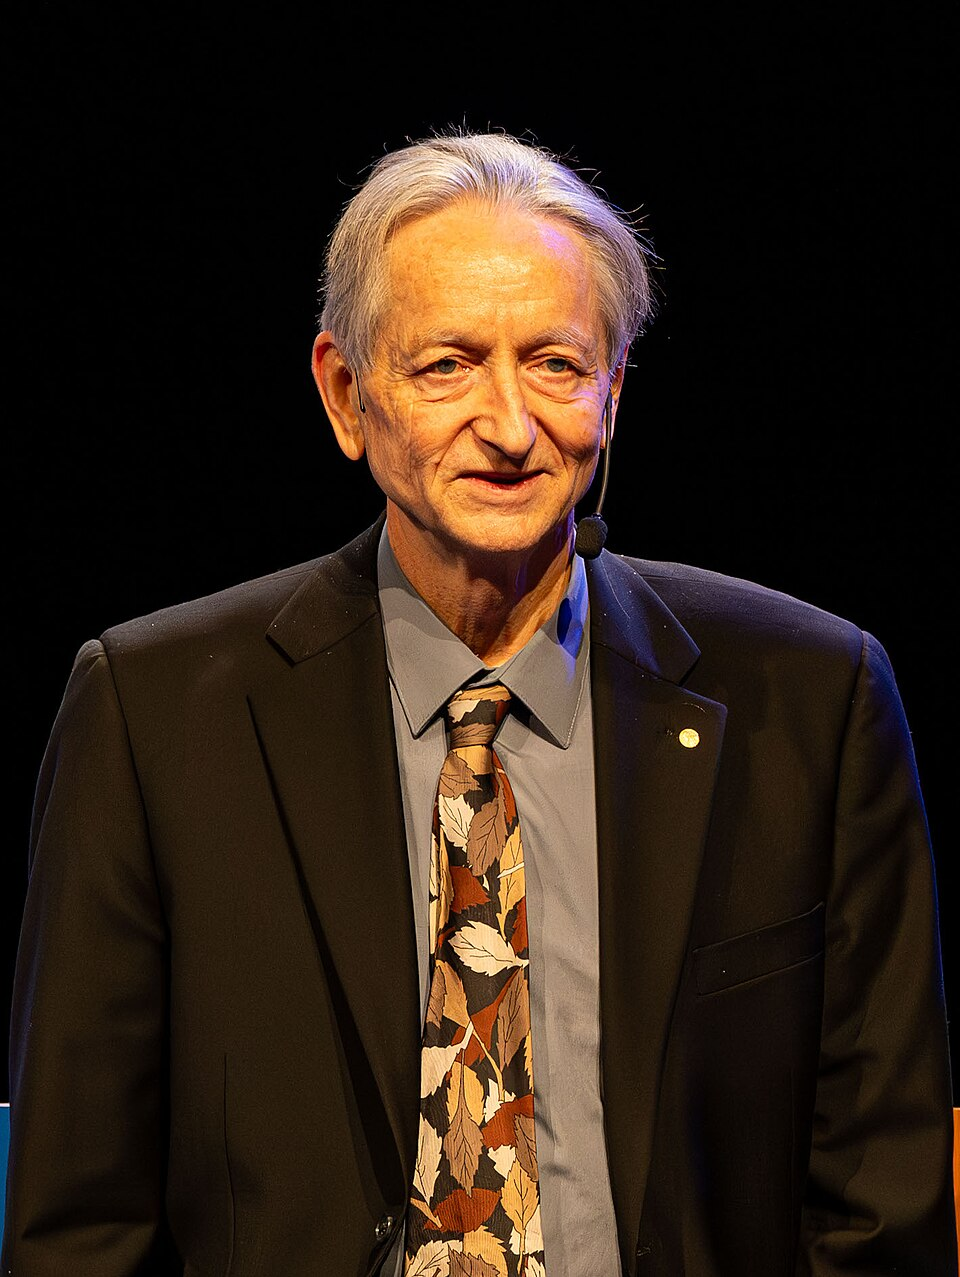
\includegraphics[height=0.48\textheight]{ch12_hinton_2024.jpg}\\[1mm]
\imgcap{Geoffrey Hinton, Nobel Prize in Physics 2024}
\imgcredit{https://commons.wikimedia.org/wiki/File:Geoffrey_E._Hinton,_2024_Nobel_Prize_Laureate_in_Physics_(cropped).jpg}{Photo: Arthur Petron (2024); CC BY-SA 4.0; Wikimedia Commons}
\end{column}
\begin{column}{0.62\textwidth}
\begin{itemize}
    \item \textbf{Statistical}: ARIMA, ETS, HAR, state space: few parameters, one model per series
    \item \textbf{Machine learning}: penalised regressions, forests, boosting on lag features, often global
    \item \textbf{Deep sequence models}: RNN, LSTM, TCN, Transformers, N-BEATS, DeepAR; backpropagation \refRHW
    \item \textbf{Foundation models}: pretrained on many series, used zero-shot (\atschlink{https://danpele.github.io/Advanced-Time-Series/EN/Courses/chapter13_foundation_models_conformal.pdf}{Chapter 13})
    \item Each generation must beat the previous one out of sample, with tests, on the same data
\end{itemize}
\end{column}
\end{columns}
\end{frame}

\begin{frame}{Four data sets, four kinds of structure}
\itemsize{\footnotesize}
\begin{center}
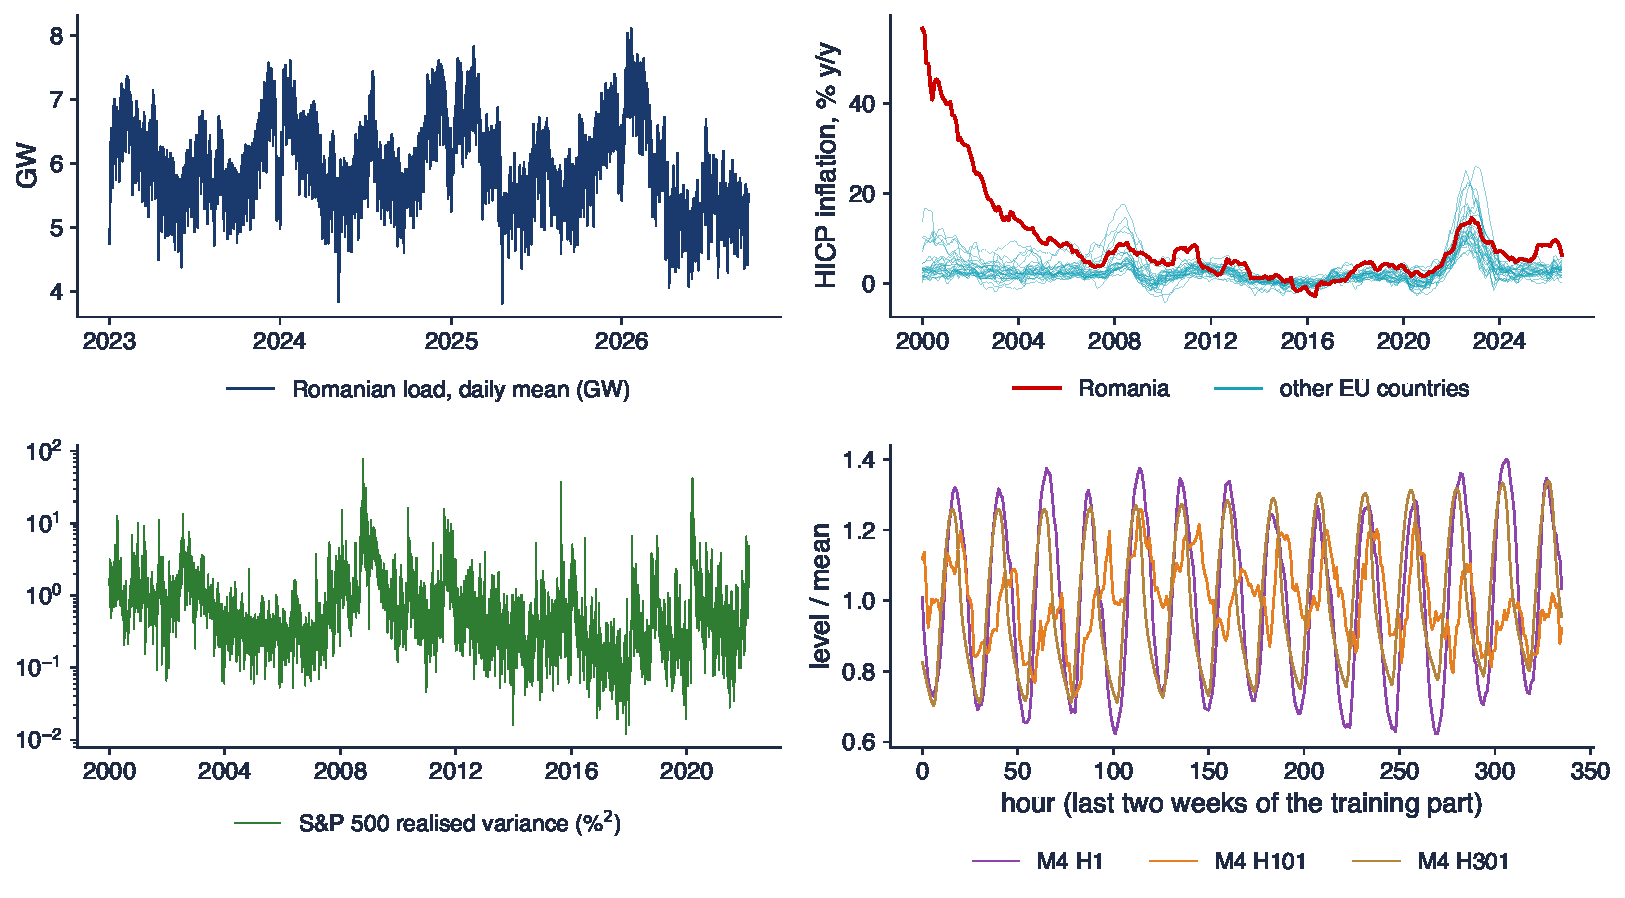
\includegraphics[width=0.97\textwidth,height=0.52\textheight,keepaspectratio]{ats_ch12_overview.pdf}
\end{center}
\vspace{-0.25cm}
\begin{itemize}
    \item Romanian load (daily mean, 6.06 GW on average); EU inflation (Romania in red); S\&P 500 realised variance (log scale); three M4 hourly series (last two weeks)
\end{itemize}
\quantlet{ATS\_ch12\_validation}{\qlurl{ATS_ch12_validation}}
\end{frame}

\begin{frame}{Interpreting the four data sets}
\itemsize{\small}
\begin{itemize}
    \item Load: strong daily and weekly seasonality, holidays, slow annual cycle: calendar structure that trees and linear models capture well
    \item Inflation: 27 short, co-moving series with a common shock in 2021--2023: the natural ground for global models and for the high-dimensional panel
    \item Realised variance: long memory and heavy tails; the HAR benchmark of \atschlink{https://danpele.github.io/Advanced-Time-Series/EN/Courses/chapter8_advanced_volatility.pdf}{Chapter 8} is hard to beat
    \item M4 hourly: many related series of the same frequency, the setting where global deep models were first shown to win
\end{itemize}
\end{frame}


%=============================================================================
\section{Learning from dependent data}
%=============================================================================

\begin{frame}{Known from TSA, and new here}
\itemsize{\small}
\begin{itemize}
    \item Known (\atschlink{https://danpele.github.io/Time-Series-Analysis/EN/Courses/chapter9_machine_learning_time_series.pdf}{TSA, Chapter 9}): lag features, walk-forward validation, leakage by example, ridge and lasso, trees, random forests, gradient boosting, a small MLP, conformal basics, M4 and M5
    \item New: the statistics behind the recipes
    \begin{itemize}
        \item generalisation under mixing; when cross-validation is valid; global models
        \item selection consistency and post-selection inference; quantile forests; constrained boosting
        \item gradients through time; attention; basis expansion; likelihood-based deep models; interpretation
    \end{itemize}
    \item Replications: Bergmeir, Hyndman and Koo (2018, Section 4); Montero-Manso and Hyndman (2021) on EU inflation; Zeng et al.\ (2023) protocol on Romanian load; the M4 hourly evaluation
\end{itemize}
\end{frame}

\begin{frame}{Risk, empirical risk and the generalisation gap (1/2)}
\itemsize{\small}
\begin{itemize}
    \item A forecast rule $f$ from a class $\mathcal F$ is judged by its expected loss under the stationary law
    \[ R(f) = \E\,\ell\big(Y_{t+h}, f(X_t)\big), \qquad \hat R_n(f) = \frac1n\sum_{t=1}^n \ell\big(y_{t+h}, f(x_t)\big) \]
    \begin{itemize}
        \item $R(f)$: \textbf{risk}; $\hat R_n(f)$: \textbf{empirical risk} on $n$ training pairs; $\ell$: loss (e.g.\ squared error); $X_t$: features known at $t$; $h$: horizon
    \end{itemize}
    \item Empirical risk minimisation (ERM) and the generalisation gap
    \[ \hat f = \arg\min_{f \in \mathcal F}\hat R_n(f), \qquad R(\hat f) - \hat R_n(\hat f) \le \sup_{f \in \mathcal F}|R(f) - \hat R_n(f)| \]
    \begin{itemize}
        \item the gap: how much worse the fitted rule does on new data than on the training data
    \end{itemize}
\end{itemize}
\end{frame}

\begin{frame}{Risk, empirical risk and the generalisation gap (2/2)}
\itemsize{\small}
\begin{itemize}
    \item i.i.d.\ data: the uniform deviation shrinks with the complexity of the class
    \[ \sup_{\mathcal F}|R - \hat R_n| = O_p\Big(\sqrt{\mathrm{complexity}(\mathcal F)/n}\Big) \]
    \begin{itemize}
        \item complexity: VC dimension or Rademacher complexity, roughly the number of patterns the class can fit
    \end{itemize}
    \item Dependent data: the $n$ observations carry less information; the bound holds with an \textbf{effective sample size} smaller than $n$
    \begin{itemize}
        \item and only if the series forgets its past fast enough: mixing
    \end{itemize}
    \item Non-stationarity (breaks, \atschlink{https://danpele.github.io/Advanced-Time-Series/EN/Courses/chapter2_structural_breaks_nonlinear_models.pdf}{Chapter 2}) adds a second gap: the future law differs from the training law; no bound covers it
\end{itemize}
\end{frame}

\begin{frame}{Mixing coefficients}
\itemsize{\small}
\begin{itemize}
    \item $\beta$-mixing: how far the distant future is from being independent of the past
    \[ \beta(a) = \sup_t\,\E\sup_{B\in\sigma(X_{t+a},\dots)}\big|P\big(B\mid\sigma(\dots,X_t)\big) - P(B)\big| \]
    \begin{itemize}
        \item $\sigma(\dots, X_t)$: the information in the past up to $t$; $\sigma(X_{t+a}, \dots)$: events $B$ of the future beyond the gap $a$; $\alpha$-mixing uses $|P(A\cap B) - P(A)P(B)|$ instead
        \item mixing: $\beta(a) \to 0$ as the gap $a \to \infty$: the far future is almost independent of the past
    \end{itemize}
    \item Stationary ARMA with continuous innovations, GARCH and Markov-switching models with ergodic chains are \textbf{geometrically} $\beta$-mixing: $\beta(a) \le Cr^a$, $C > 0$, $0 < r < 1$
    \begin{itemize}
        \item long memory (\atschlink{https://danpele.github.io/Advanced-Time-Series/EN/Courses/chapter10_long_memory_rough_volatility.pdf}{Chapter 10}) is not geometrically mixing: the effective sample size shrinks much more
    \end{itemize}
    \item Mixing is assumed, rarely tested: it is a statement about the data-generating process, not about the sample
\end{itemize}
\end{frame}

\begin{frame}{Blocking and a generalisation bound}
\itemsize{\small}
\begin{itemize}
    \item \refYu: split the sample into $2\mu$ alternating blocks of length $a$; under $\beta$-mixing the odd blocks behave like $\mu$ \textbf{independent} blocks up to an error $\mu\,\beta(a)$
    \begin{itemize}
        \item i.i.d.\ tools then apply with $\mu = n/(2a)$ observations instead of $n$
    \end{itemize}
    \item \refMR: for a uniformly stable learner, with probability at least $1 - \delta$
    \[ R(\hat f) \le \hat R_n(\hat f) + O(\kappa_n a) + O\Big(\sqrt{\log(1/\delta')/\mu}\Big), \qquad \delta' = \delta - 2(\mu - 1)\beta(a) \]
    \begin{itemize}
        \item $\kappa_n$: uniform stability, the largest change of the loss when one training point changes; $\delta$: confidence level
        \item trade-off in $a$: long blocks make $\beta(a)$ small but leave few blocks $\mu$; ridge and regularised models are uniformly stable, deep networks trained by SGD only approximately
    \end{itemize}
    \item The same blocking idea gives blocked bootstrap (\atschlink{https://danpele.github.io/Advanced-Time-Series/EN/Courses/chapter0_refresher_inference.pdf}{Chapter 0}) and blocked cross-validation
\end{itemize}
\end{frame}

\begin{frame}{Cross-validation for time series: the schemes}
\itemsize{\small}
\begin{itemize}
    \item \textbf{Random K-fold}: rows of the lag matrix $(y_t; y_{t-1},\dots,y_{t-p})$ assigned to folds at random
    \item \textbf{Non-dependent CV} \refBHK: the same folds, but training rows within $p$ lags of a test row are removed
    \item \textbf{Blocked K-fold} and \textbf{hv-block} \refBCN, \refRac: contiguous test blocks, a gap of $h$ rows (purge) on each side
    \item \textbf{Out-of-sample (OOS)} and \textbf{rolling origin}: test only on the end; the only scheme that mimics real use, at the price of a high variance
    \item The question is not which scheme is ``correct'' but which estimates the future risk with small bias and small variance
\end{itemize}
\end{frame}

\begin{frame}{When K-fold is valid: Bergmeir, Hyndman and Koo (2018)}
\itemsize{\small}
\begin{itemize}
    \item A nonlinear autoregression with \textbf{uncorrelated} errors \refBHK
    \[ y_t = g(y_{t-1},\dots,y_{t-p}; \theta) + \varepsilon_t \]
    \begin{itemize}
        \item $g$: any regression function (linear, tree, network) with parameters $\theta$; $p$: number of lags; $\varepsilon_t$: errors, $\Cov(\varepsilon_t, \varepsilon_s) = 0$ for $t \ne s$
        \item the rows of the lag matrix are then exchangeable enough: a test row shares no error with a training row
        \item result: the K-fold estimate of the MSE is asymptotically unbiased, and has a lower variance than OOS because every row is used
    \end{itemize}
    \item It fails when the residuals are autocorrelated: an under-specified model, overlapping $h$-step targets, or features that identify time
    \begin{itemize}
        \item then a test error is predictable from the neighbouring training errors: optimistic estimates
    \end{itemize}
    \item Practical rule: check the residual ACF of the fitted model (Ljung--Box, \atschlink{https://danpele.github.io/Time-Series-Analysis/EN/Courses/chapter2_arma_models.pdf}{TSA, Chapter 2}) before trusting random K-fold
\end{itemize}
\end{frame}

\begin{frame}{Replication design: Bergmeir, Hyndman and Koo (2018, Section 4)}
\itemsize{\small}
\begin{itemize}
    \item Series of length 200: in-set 140, out-set 60; models AR(1)--AR(5) by OLS; one-step forecasts
    \item Procedures on the in-set: 5-fold CV, LOOCV, non-dependent CV ($p = 5$), OOS (last 20\%); ``true'' error: the model on the whole in-set, RMSE on the out-set
    \item 1\,000 trials per DGP: stationary AR(3) with random coefficients, invertible MA(1), and a seasonal AR fitted to US accidental deaths 1973--1978 ($\phi = 0.76$, $\Phi_{12} = 0.85$) as the counterexample
    \item Precision and bias of each procedure
    \[ \mathrm{MAPAE} = \mathrm{mean}\,|\widehat{PE} - PE|, \qquad \mathrm{MPAE} = \mathrm{mean}\,(\widehat{PE} - PE) \]
    \begin{itemize}
        \item $PE$: the true prediction error (RMSE on the out-set); $\widehat{PE}$: its estimate by the procedure; averages over the trials; MPAE $< 0$: optimistic
    \end{itemize}
\end{itemize}
\end{frame}

\begin{frame}{Which validation estimates the future error?}
\itemsize{\footnotesize}
\begin{center}
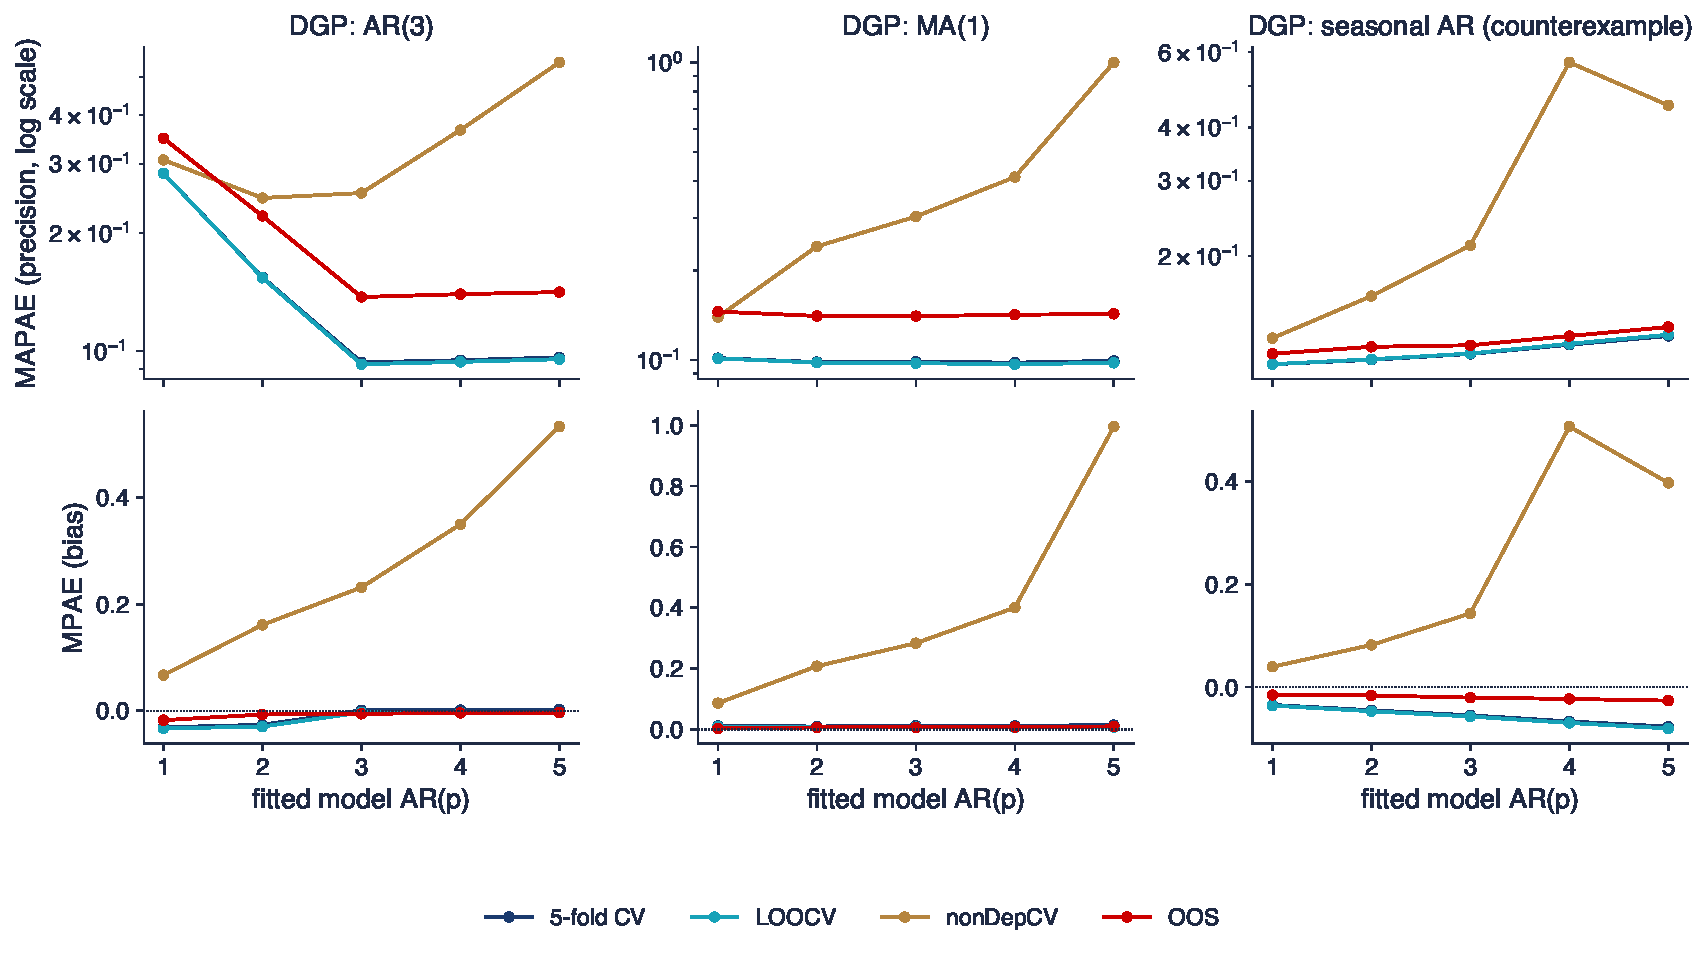
\includegraphics[width=0.97\textwidth,height=0.58\textheight,keepaspectratio]{ats_ch12_cv_bhk.pdf}
\end{center}
\vspace{-0.25cm}
\begin{itemize}
    \item Top: precision (log scale); bottom: bias, by fitted AR order and data-generating process
\end{itemize}
\quantlet{ATS\_ch12\_validation}{\qlurl{ATS_ch12_validation}}
\end{frame}

\begin{frame}{Interpreting the replication}
\itemsize{\small}
\begin{itemize}
    \item AR(3) data, AR(3) model: 5-fold CV has MAPAE 0.094 against 0.137 for OOS, bias 0.001: as in the paper, CV is unbiased and more precise
    \item Under-specified AR(1) on AR(3) data: residuals are autocorrelated and CV loses its edge (MAPAE 0.284 against 0.349)
    \item Seasonal counterexample: every AR($p \le 5$) misses lag 12; CV is biased down (MPAE \ensuremath{-}0.077 for AR(5)) and no more precise than OOS (0.130 against 0.136)
    \item Non-dependent CV removes so many rows that its models are poor: bias 0.232 for AR(3); the price of independence is paid in data
\end{itemize}
\end{frame}

\begin{frame}{Leakage through overlapping targets and time features}
\itemsize{\small}
\begin{itemize}
    \item Target $z_t = \frac1h\sum_{j=1}^h y_{t+j}$ (a month of volatility, a quarter of sales): $\mathrm{corr}(z_t, z_{t+1}) \ge (h - 1)/h$ when $y$ is white noise, more when $y$ is persistent
    \begin{itemize}
        \item a random fold puts $z_{t-1}$ and $z_{t+1}$ in training when $z_t$ is tested: the answer is almost in the training set
    \end{itemize}
    \item A time index or a date feature lets a flexible learner \textbf{locate} the test row between its neighbours
    \item Simulation: AR(1) with $\phi = 0.9$, $h = 20$, a random forest on $y_t,\dots,y_{t-4}$ and a time index; 60 replications; ratio of the estimated to the true RMSE on new data
\end{itemize}
\end{frame}

\begin{frame}{How optimistic is each validation scheme?}
\itemsize{\footnotesize}
\begin{center}
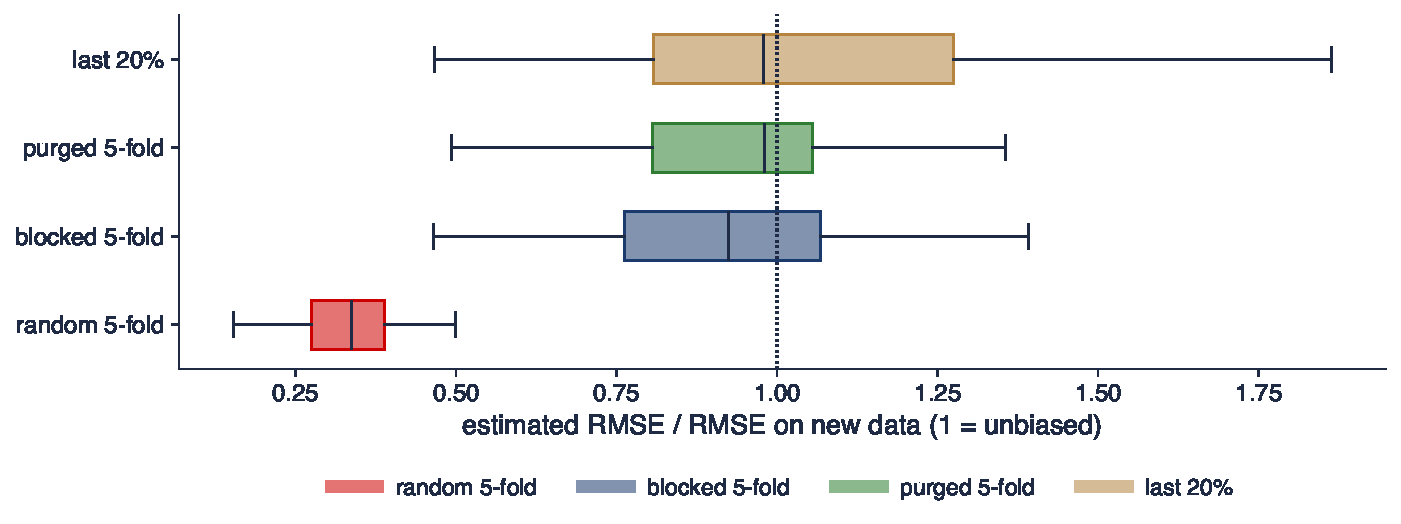
\includegraphics[width=0.97\textwidth,height=0.46\textheight,keepaspectratio]{ats_ch12_leakage.pdf}
\end{center}
\vspace{-0.25cm}
\begin{itemize}
    \item Ratio 1: the scheme estimates the error on new data without bias; below 1: optimistic
\end{itemize}
\quantlet{ATS\_ch12\_validation}{\qlurl{ATS_ch12_validation}}
\end{frame}

\begin{frame}{Interpreting the leakage experiment}
\itemsize{\small}
\begin{itemize}
    \item Random 5-fold: median ratio 0.34 (quartiles 0.28--0.39): it claims an error three times smaller than the truth
    \item Blocked 5-fold 0.92, purged 5-fold 0.98, last 20\% 0.98: contiguity and the purge remove most of the bias
    \item The interior blocks still let the forest interpolate in time; only the last block reproduces extrapolation into the future
    \item Rule: purge at least $h$ rows around every test block and drop time indices unless the trend is modelled explicitly
\end{itemize}
\end{frame}

\begin{frame}{Recap: Learning from dependent data}
\itemsize{\small}
\begin{itemize}
    \item Generalisation bounds hold with an effective sample size set by mixing; blocking is the common tool
    \item Random K-fold is valid for autoregressions with uncorrelated errors, and then better than OOS
    \item Overlapping targets, under-fitting and time features break it: block, purge, and keep a final untouched period
\end{itemize}
\end{frame}


%=============================================================================
\section{Global models and high-dimensional regression}
%=============================================================================

\begin{frame}{Local and global models}
\itemsize{\small}
\begin{itemize}
    \item \textbf{Local}: one model per series, $\hat y_{i,t+h} = f_i(y_{i,t}, y_{i,t-1},\dots)$; \textbf{global}: one function for all series, $\hat y_{i,t+h} = f(y_{i,t}, y_{i,t-1},\dots)$
    \begin{itemize}
        \item global models pool $N \times T$ rows: far more data per parameter
    \end{itemize}
    \item \refMMH: for any set of series a global model exists that forecasts as well as the local ones; global models can afford \textbf{longer memory} and more complexity
    \begin{itemize}
        \item their bound: the complexity of a global model grows with $NT$, that of $N$ local models with $T$ each
    \end{itemize}
    \item The M4 and M5 winners were global (\refSmyl; LightGBM in \refMfiveA): pooling, not depth, was the common ingredient
    \item Scaling matters: series of different levels are divided by their own scale before pooling (inflation rates share a scale)
\end{itemize}
\end{frame}

\begin{frame}{Design: EU inflation, local against global}
\itemsize{\small}
\begin{itemize}
    \item Annual HICP inflation of the 27 EU countries; direct forecasts $h = 1$ and $h = 12$ months ahead from AR($p$) models, $p \in \{1, 2, 3, 6, 12, 18, 24, 36\}$
    \item Rolling window of 120 months; forecast origins from January 2015 (139 origins for $h = 1$)
    \item Local: 27 OLS regressions per origin; global: one pooled OLS (the same coefficients for all countries), as in \refMMH
    \item Loss: RMSE in percentage points; DM test on the cross-country average loss differential (HLN correction, \atschlink{https://danpele.github.io/Advanced-Time-Series/EN/Courses/chapter1_forecast_evaluation.pdf}{Chapter 1})
\end{itemize}
\end{frame}

\begin{frame}{Memory helps global models and hurts local ones}
\itemsize{\footnotesize}
\begin{center}
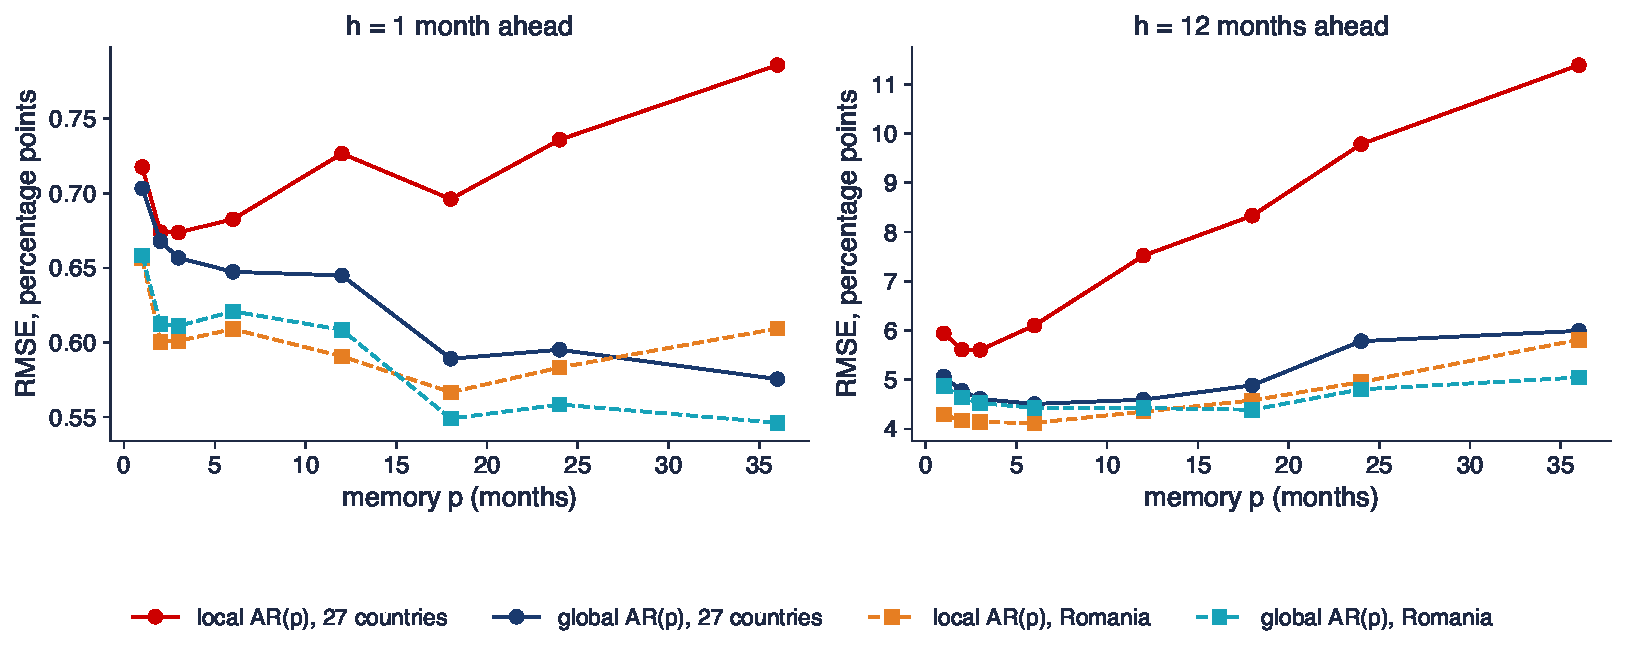
\includegraphics[width=0.97\textwidth,height=0.5\textheight,keepaspectratio]{ats_ch12_global_local.pdf}
\end{center}
\vspace{-0.25cm}
\begin{itemize}
    \item RMSE against the memory $p$; circles: average over the 27 countries; squares: Romania
\end{itemize}
\quantlet{ATS\_ch12\_global\_models}{\qlurl{ATS_ch12_global_models}}
\end{frame}

\begin{frame}{Interpreting local and global}
\itemsize{\small}
\begin{itemize}
    \item $h = 1$: local RMSE is best at $p = 3$ (0.67) and then deteriorates; global keeps improving up to $p = 36$ (0.58); DM on the 27-country average \ensuremath{-}4.40 ($p$ $<$0.001)
    \item $h = 12$: the 2021--2023 surge dominates; local AR(36) reaches 11.39 against 5.99 global; best global 4.51 against best local 5.60, DM \ensuremath{-}1.09 ($p$ 0.277)
    \item Romania alone: the global model helps at $h = 1$ with long memory (0.55 against 0.61 at $p = 36$), not significantly (DM $p$ 0.19)
    \item Lesson of Montero-Manso and Hyndman confirmed: pooling buys memory; for a single series the gain is real but hard to prove
\end{itemize}
\end{frame}

\begin{frame}{The lasso (1/2): optimality conditions}
\itemsize{\small}
\begin{itemize}
    \item \refTib: least squares with an $\ell_1$ penalty
    \[ \hat\beta = \arg\min_\beta \frac1{2n}\|y - X\beta\|^2 + \lambda\|\beta\|_1, \qquad \|\beta\|_1 = \sum_j|\beta_j| \]
    \begin{itemize}
        \item $y$: $n \times 1$ target; $X$: $n \times p$ predictors, columns $x_j$; $\lambda \ge 0$: penalty, the larger the more coefficients set to zero
        \item Karush--Kuhn--Tucker (KKT): $\frac1n x_j'(y - X\hat\beta) = \lambda\,\mathrm{sign}(\hat\beta_j)$ if $\hat\beta_j \ne 0$, and $|\frac1n x_j'(y - X\hat\beta)| \le \lambda$ otherwise
    \end{itemize}
    \item Orthonormal predictors ($X'X = nI$): soft thresholding of the OLS coefficient $z_j$
    \[ \hat\beta_j^{\mathrm{lasso}} = \mathrm{sign}(z_j)\,(|z_j| - \lambda)_+, \qquad \hat\beta_j^{\mathrm{ridge}} = \frac{z_j}{1 + \lambda} \]
    \begin{itemize}
        \item $(u)_+ = \max(u, 0)$; the lasso selects (sets small $z_j$ to zero), ridge only shrinks
    \end{itemize}
\end{itemize}
\end{frame}

\begin{frame}{The lasso (2/2): prediction and selection}
\itemsize{\small}
\begin{itemize}
    \item Prediction: with $s$ non-zero coefficients and a restricted eigenvalue $\kappa$, for $\lambda \asymp \sigma\sqrt{\log p/n}$
    \[ \frac1n\|X(\hat\beta - \beta)\|^2 = O_p\Big(\frac{s\log p}{n\kappa^2}\Big) \]
    \begin{itemize}
        \item $\sigma$: error standard deviation; $\kappa$: how far $X$ is from collinearity on sparse directions; time series: the same rate for stable VARs \refBM, heavy-tailed errors \refMM
    \end{itemize}
    \item Selection is harder than prediction: sign consistency needs the \textbf{irrepresentable condition} \refZY
    \[ \big\|X_{S^c}'X_S(X_S'X_S)^{-1}\mathrm{sign}(\beta_S)\big\|_\infty < 1 \]
    \begin{itemize}
        \item $S$: the set of relevant predictors, $S^c$: the others; it fails when relevant and irrelevant predictors are correlated (neighbouring countries, lags)
    \end{itemize}
\end{itemize}
\end{frame}

\begin{frame}{Adaptive lasso and elastic net}
\itemsize{\small}
\begin{itemize}
    \item \textbf{Adaptive lasso} \refZou: coefficient-specific weights from a first-step estimate
    \[ \lambda\sum_j w_j|\beta_j|, \qquad w_j = 1/|\tilde\beta_j|^\gamma \]
    \begin{itemize}
        \item $\tilde\beta_j$: first-step estimate (OLS, ridge); $\gamma > 0$; large coefficients are penalised little, small ones a lot
        \item \textbf{oracle property}: consistent selection and $\sqrt n$-normal estimates of the non-zero coefficients, without the irrepresentable condition
    \end{itemize}
    \item \textbf{Elastic net} \refZH: a mix of the lasso and ridge penalties
    \[ \lambda\Big(\alpha\|\beta\|_1 + \frac{1 - \alpha}2\|\beta\|_2^2\Big) \]
    \[ \hat\beta_j = \frac{\mathrm{sign}(z_j)(|z_j| - \lambda\alpha)_+}{1 + \lambda(1 - \alpha)} \ (X'X = nI) \]
    \begin{itemize}
        \item $\alpha \in [0, 1]$: $\alpha = 1$ lasso, $\alpha = 0$ ridge; grouping effect: correlated predictors enter together instead of one being chosen at random
    \end{itemize}
    \item The penalty is tuned by CV: with $h$-step targets use blocked folds with a purge of $h$ periods (Section 1)
\end{itemize}
\end{frame}

\begin{frame}{Inference after selection}
\itemsize{\small}
\begin{itemize}
    \item Naive practice: select with the lasso, then report OLS $t$-statistics of the selected variables: the $p$-values are \textbf{too small}
    \begin{itemize}
        \item the same data chose the model and test it: the distribution of $\hat\beta$ is conditional on being selected
    \end{itemize}
    \item Remedies: \textbf{PoSI} intervals valid for any selection \refBerk; \textbf{exact conditional} intervals for the lasso (a polyhedral selection event) \refLSST
    \item For one coefficient of interest (a policy rate, a foreign shock): \textbf{double selection} \refBCH: lasso of $y$ on the controls, lasso of the regressor of interest on the controls, OLS on the union
    \begin{itemize}
        \item with HAC standard errors for time series (\atschlink{https://danpele.github.io/Advanced-Time-Series/EN/Courses/chapter0_refresher_inference.pdf}{Chapter 0})
    \end{itemize}
    \item For forecasting, selection is a means: judge it by out-of-sample loss and by the stability of what is selected
\end{itemize}
\end{frame}

\begin{frame}{Design: Romanian inflation from the EU panel}
\itemsize{\small}
\begin{itemize}
    \item Target: Romanian annual HICP inflation 12 months ahead; window 120 months, re-estimation every 3 months; 128 forecasts (January 2016 -- August 2026)
    \item Features: 3 own lags (never penalised) and 3 lags of the 26 other countries: 78 penalised predictors for about 105 observations
    \item Models: AR(3) (benchmark), ridge, lasso, adaptive lasso, elastic net ($\alpha = 0.5$), post-lasso OLS, global AR(12) of the panel; penalty by blocked 5-fold CV with a 12-month purge
    \item In the spirit of the data-rich inflation literature \refMVVZ, \refGCLSS, with the EU panel as the data set
\end{itemize}
\end{frame}

\begin{frame}{What the panel lasso selects, and what it delivers}
\itemsize{\footnotesize}
\begin{center}
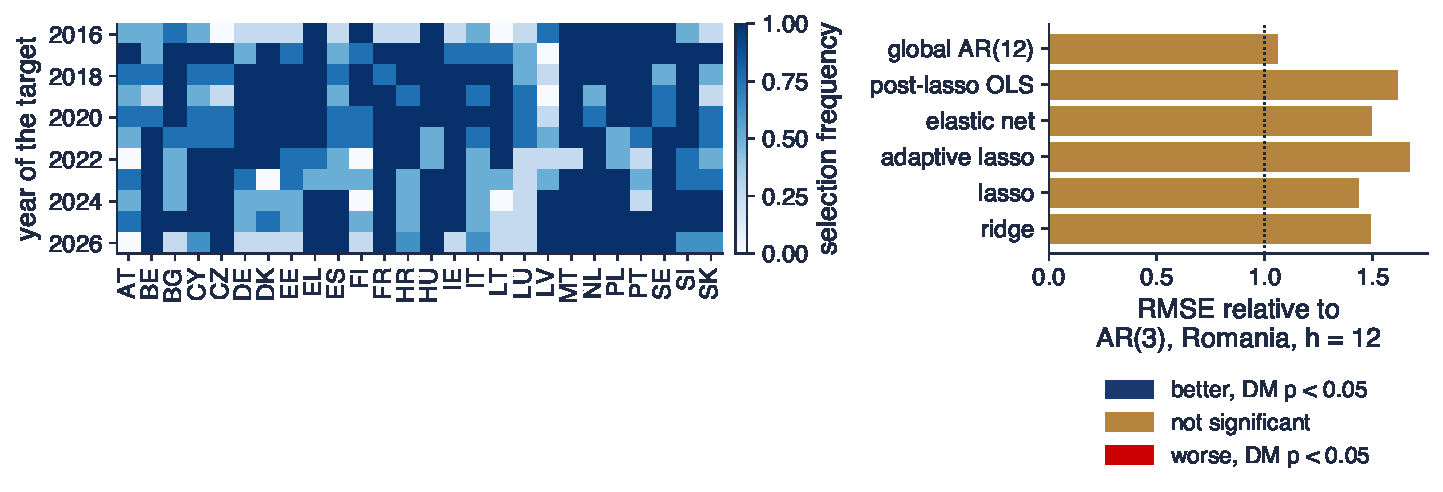
\includegraphics[width=0.97\textwidth,height=0.48\textheight,keepaspectratio]{ats_ch12_ro_lasso.pdf}
\end{center}
\vspace{-0.25cm}
\begin{itemize}
    \item Left: share of forecast origins in each year at which a country enters the lasso; right: RMSE relative to AR(3), colour by the DM test
\end{itemize}
\quantlet{ATS\_ch12\_global\_models}{\qlurl{ATS_ch12_global_models}}
\end{frame}

\begin{frame}{Interpreting the panel lasso}
\itemsize{\small}
\begin{itemize}
    \item Selection is unstable: median 34 of 78 predictors (from 15 to 61); the most frequent are EL, NL, MT, not Romania's neighbours
    \item Accuracy: AR(3) RMSE 4.13; lasso 1.44, adaptive lasso 1.67, elastic net 1.49, ridge 1.49 times as large; global AR(12) 1.06
    \item None of the differences is significant (DM $p$ from 0.20 to 0.39): about 10 independent 12-month periods, one dominated by the 2022 surge
    \item High dimension with 105 observations of a persistent target: CV picks small penalties, the panel fits past co-movement that does not repeat; parsimony wins here
\end{itemize}
\end{frame}

\begin{frame}{Recap: Global models and high dimension}
\itemsize{\small}
\begin{itemize}
    \item Global models pool many series and can afford long memory; on EU inflation they win at one month
    \item The lasso predicts well under sparsity and restricted eigenvalues; it selects well only under the irrepresentable condition; adaptive lasso and elastic net relax it
    \item Report selection stability and use PoSI, exact or double-selection inference, never naive $t$-statistics
\end{itemize}
\end{frame}


%=============================================================================
\section{Tree ensembles in depth}
%=============================================================================

\begin{frame}{Bagging: the variance of an average}
\itemsize{\small}
\begin{itemize}
    \item Average of $B$ predictors $\hat f_b(x)$ trained on bootstrap samples \refBreA
    \[ \Var\Big(\frac1B\sum_{b=1}^B\hat f_b(x)\Big) = \frac1{B^2}\big(B\sigma^2 + B(B - 1)\rho\sigma^2\big) = \rho\sigma^2 + \frac{1 - \rho}B\sigma^2 \]
    \begin{itemize}
        \item $\sigma^2$: variance of one predictor; $\rho$: pairwise correlation of two predictors (over the data and the randomisation)
        \item more trees remove only the second term; the floor $\rho\sigma^2$ is lowered only by \textbf{decorrelating} the trees
    \end{itemize}
    \item \textbf{Random forests} \refBreB: a random subset of $m_{\mathrm{try}}$ features at each split lowers $\rho$ at the cost of a little bias
    \begin{itemize}
        \item theory: consistency for additive regression \refSBV; honest trees (separate samples for splits and leaf values) give asymptotically Normal forecasts \refWA
    \end{itemize}
    \item Trees cannot extrapolate: a forecast is an average of past targets, so trends and level shifts need differencing or a linear part
\end{itemize}
\end{frame}

\begin{frame}{Quantile regression forests}
\itemsize{\small}
\begin{itemize}
    \item \refMei: keep \textbf{all} training targets in the leaves and weight them by how often they share a leaf with $x$
    \[ w_i(x) = \frac1B\sum_{b=1}^B \frac{\mathbf 1\{x_i \in L_b(x)\}}{|L_b(x)|}, \qquad \hat F(y\mid x) = \sum_i w_i(x)\,\mathbf 1\{y_i \le y\} \]
    \begin{itemize}
        \item $L_b(x)$: the leaf of tree $b$ that contains $x$; $|L_b(x)|$: number of training points in it; $\sum_i w_i(x) = 1$
        \item $\hat F(y\mid x)$: estimated conditional distribution function; quantile $\hat q_\tau(x) = \inf\{y: \hat F(y\mid x) \ge \tau\}$
    \end{itemize}
    \item The same forest gives every quantile: no crossing, no refit per level
    \begin{itemize}
        \item consistent for the conditional distribution under regularity conditions; a random forest is an adaptive nearest-neighbour method
    \end{itemize}
    \item Evaluation with the pinball loss and coverage (\atschlink{https://danpele.github.io/Advanced-Time-Series/EN/Courses/chapter1_forecast_evaluation.pdf}{Chapter 1}): the bands are honest only if the forest was trained on data like the future
\end{itemize}
\end{frame}

\begin{frame}{Gradient boosting (1/2): functional gradient descent}
\itemsize{\small}
\begin{itemize}
    \item \refFri: add small trees, each fitted to the negative gradient of the loss at the current fit
    \[ F_m = F_{m-1} + \nu\,h_m, \qquad g_i = -\frac{\partial\ell(y_i, F)}{\partial F}\Big|_{F = F_{m-1}(x_i)} \]
    \begin{itemize}
        \item $F_m$: the fit after $m$ trees; $h_m$: a small tree fitted to $(x_i, g_i)$; $\nu \in (0, 1]$: learning rate (shrinkage): smaller steps, more trees, lower variance
        \item squared loss: $g_i$ = residual; pinball loss: $g_i = \tau - \mathbf 1\{y_i < F\}$ (quantile boosting)
    \end{itemize}
\end{itemize}
\end{frame}

\begin{frame}{Gradient boosting (2/2): second order, histograms, constraints}
\itemsize{\small}
\begin{itemize}
    \item Second order \refCG: optimal leaf value and the gain of a split
    \[ w^* = -\frac{G}{H + \lambda}, \qquad \mathrm{gain} = \frac12\Big[\frac{G_L^2}{H_L + \lambda} + \frac{G_R^2}{H_R + \lambda} - \frac{G^2}{H + \lambda}\Big] - \gamma \]
    \begin{itemize}
        \item $G$, $H$: sums of the first and second derivatives of the loss over the points of a leaf ($L$, $R$: left and right child); $\lambda$: penalty on leaf values; $\gamma$: cost of a split
    \end{itemize}
    \item LightGBM \refKeA: features binned into histograms (at most 255 bins), leaf-wise growth, gradient-based one-side sampling; scikit-learn HistGradientBoosting (used here) follows the same construction
    \item Monotone constraints: a split is allowed only if the left and right leaf values respect the order, and children inherit bounds; the fit is then monotone in that feature everywhere
\end{itemize}
\end{frame}

\begin{frame}{Design: Romanian day-ahead load}
\itemsize{\small}
\begin{columns}[T]
\begin{column}{0.34\textwidth}
\centering
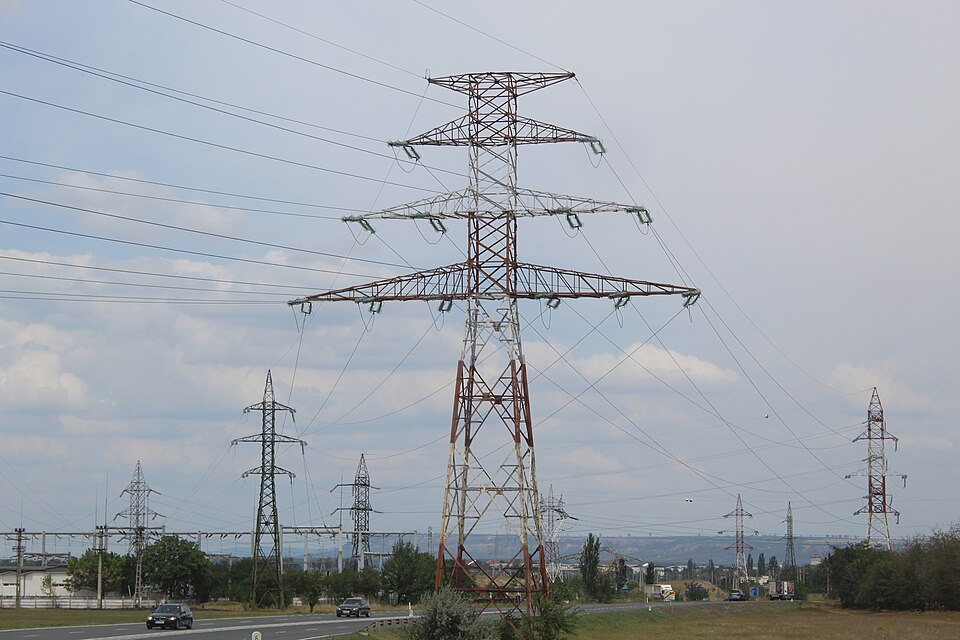
\includegraphics[height=0.42\textheight]{ch12_marasesti_750kv_2022.jpg}\\[1mm]
\imgcap{750 kV line at Mărășești, Romania}
\imgcredit{https://commons.wikimedia.org/wiki/File:750_kV_electricity_tower_at_M\%C4\%83r\%C4\%83\%C8\%99e\%C8\%99ti,_Romania.jpg}{Photo: TrainSimFan (2022); CC BY-SA 4.0; Wikimedia Commons}
\end{column}
\begin{column}{0.64\textwidth}
\begin{itemize}
    \item Forecast the 24 hourly loads of day $d + 1$ with data up to day $d$; evaluation 638 days, January 2025 -- September 2026
    \item Benchmark: the expert ARX of \atschlink{https://danpele.github.io/Advanced-Time-Series/EN/Courses/chapter1_forecast_evaluation.pdf}{Chapter 1} (\refZW): one regression per hour, 364-day window, refitted daily
    \item Global learners (one model for all hours) on the same lags, hour, weekday, Romanian holidays, annual cycle; refitted monthly on all earlier data: RF with QRF bands, HGB, HGB increasing in the three load lags, quantile HGB
    \item Losses: MAE, average pinball over the deciles, 80\% coverage; DM against ARX and MCS (\atschlink{https://danpele.github.io/Advanced-Time-Series/EN/Courses/chapter1_forecast_evaluation.pdf}{Chapter 1})
\end{itemize}
\end{column}
\end{columns}
\end{frame}

\begin{frame}{Trees against the expert ARX}
\itemsize{\footnotesize}
\begin{center}
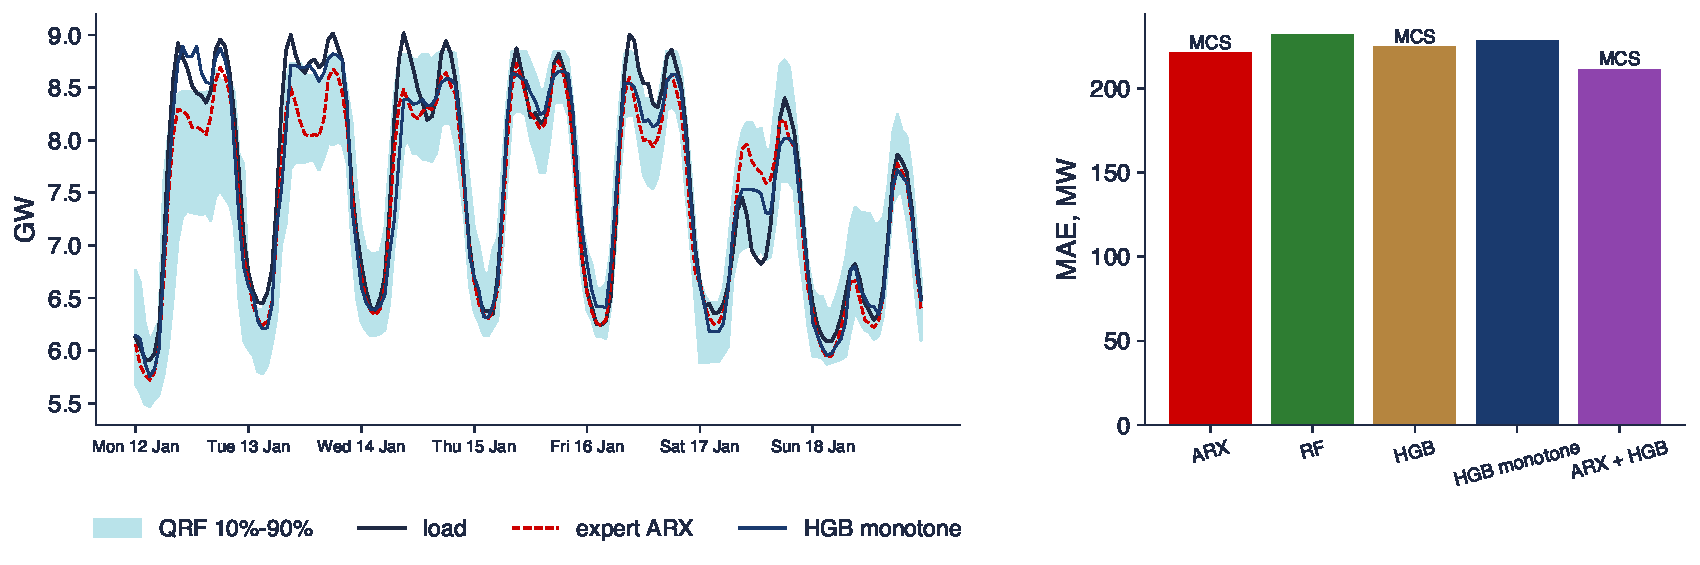
\includegraphics[width=0.97\textwidth,height=0.46\textheight,keepaspectratio]{ats_ch12_load_trees.pdf}
\end{center}
\vspace{-0.25cm}
\begin{itemize}
    \item Left: one January week with QRF 10\%--90\% bands; right: MAE in MW, MCS marks the models in the 90\% Model Confidence Set
\end{itemize}
\quantlet{ATS\_ch12\_trees}{\qlurl{ATS_ch12_trees}}
\end{frame}

\begin{frame}{Interpreting the load comparison}
\itemsize{\small}
\begin{itemize}
    \item MAE (MW): ARX 221, RF 232, HGB 225, monotone HGB 228; the forest is significantly worse (DM 2.84), boosting is not significantly different from ARX
    \item The equal-weight average of ARX and boosting: 211 MW, DM \ensuremath{-}3.36 ($p$ $<$0.001), the only model in the MCS: combination beats selection (\atschlink{https://danpele.github.io/Advanced-Time-Series/EN/Courses/chapter1_forecast_evaluation.pdf}{Chapter 1})
    \item Quantiles: pinball (MW) ARX 89.1, quantile HGB 89.5, QRF 92.8; 80\% coverage 78\%, 61\%, 83\%: quantile boosting is sharp but under-covers, QRF over-covers
    \item A daily-refitted linear model with the right structure is a strong baseline; trees add value as a complement, not as a replacement
\end{itemize}
\end{frame}

\begin{frame}{Monotone constraints in practice}
\itemsize{\footnotesize}
\begin{center}
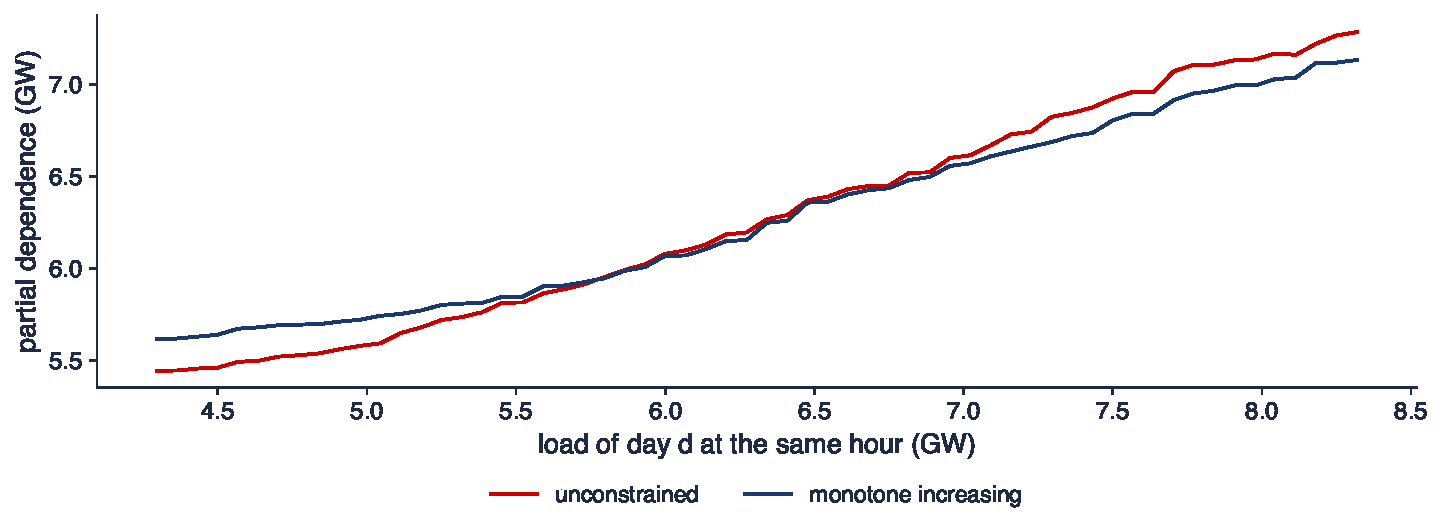
\includegraphics[width=0.97\textwidth,height=0.46\textheight,keepaspectratio]{ats_ch12_monotone.pdf}
\end{center}
\vspace{-0.25cm}
\begin{itemize}
    \item Partial dependence of the boosted forecast on the load of day $d$ at the same hour, trained on 2023--2024
\end{itemize}
\quantlet{ATS\_ch12\_trees}{\qlurl{ATS_ch12_trees}}
\end{frame}

\begin{frame}{Interpreting the constraint}
\itemsize{\small}
\begin{itemize}
    \item Unconstrained: 3 decreasing steps (the largest 7.5 MW): more load yesterday would sometimes mean less load tomorrow, a fit to noise
    \item Constrained: monotone by construction; total range 1.52 GW against 1.84 GW: part of the effect moves to the other lags
    \item Accuracy barely changes (228 against 225 MW); the gain is plausibility and robustness at the edges of the data
    \item Constraints are how economic knowledge enters a black box: sign restrictions, as in \atschlink{https://danpele.github.io/Advanced-Time-Series/EN/Courses/chapter3_structural_var_local_projections.pdf}{Chapter 3}, but for nonlinear learners
\end{itemize}
\end{frame}

\begin{frame}{Recap: Tree ensembles}
\itemsize{\small}
\begin{itemize}
    \item Bagging and forests reduce variance down to the floor $\rho\sigma^2$; decorrelation, not the number of trees, lowers it
    \item QRF gives the whole conditional distribution from one forest; boosting fits gradients, with second-order leaves and histograms in LightGBM
    \item On Romanian load, trees match but do not beat the expert ARX; their combination wins
\end{itemize}
\end{frame}


%=============================================================================
\section{Deep learning for sequences}
%=============================================================================

\begin{frame}{From the MLP to sequence models}
\itemsize{\small}
\begin{columns}[T]
\begin{column}{0.32\textwidth}
\centering
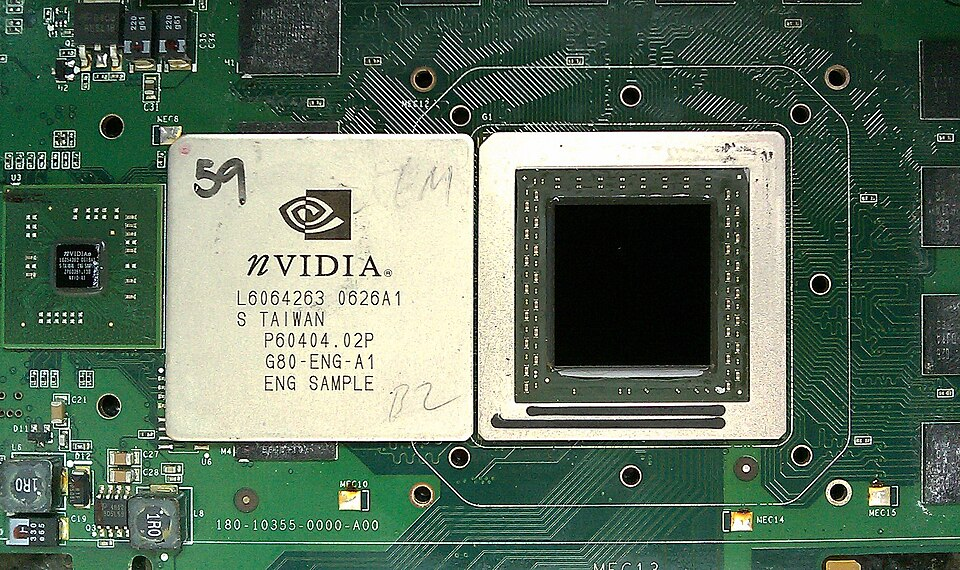
\includegraphics[height=0.3\textheight]{ch12_nvidia_g80.jpg}\\[1mm]
\imgcap{NVIDIA G80, the first CUDA graphics processor (2006)}
\imgcredit{https://commons.wikimedia.org/wiki/File:NVIDIA_G80_GPU_Core.jpg}{Photo: Hyins (2011); public domain; Wikimedia Commons}
\end{column}
\begin{column}{0.66\textwidth}
\begin{itemize}
    \item An MLP on a window of $L$ lags is a nonlinear AR($L$)
    \[ \hat y_{t+h} = W_2\,\sigma(W_1x_t + b_1) + b_2 \]
    \begin{itemize}
        \item $x_t$: the $L$ most recent values; $W_1$, $W_2$: weight matrices; $b_1$, $b_2$: biases; $\sigma$: activation applied elementwise (ReLU or tanh)
    \end{itemize}
    \item Training: backpropagation \refRHW\ with Adam \refKB; early stopping on the last block of the training sample; inputs standardised with training moments only
    \item Universal approximation says nothing about data needs: with a few thousand daily observations a network has little room over a linear model
    \item Sequence models share weights across time: recurrence (RNN), convolution (TCN) or attention (Transformer)
\end{itemize}
\end{column}
\end{columns}
\end{frame}

\begin{frame}{Recurrent networks and backpropagation through time (1/2)}
\itemsize{\small}
\begin{itemize}
    \item Elman RNN: a hidden state updated by the same weights at every step
    \[ h_t = \tanh(W h_{t-1} + U x_t + b), \qquad \hat y_t = V h_t \]
    \begin{itemize}
        \item $h_t$: hidden state, a learned summary of the past (like the Kalman state of \atschlink{https://danpele.github.io/Advanced-Time-Series/EN/Courses/chapter6_state_space_models_bayesian_filtering.pdf}{Chapter 6}); $x_t$: input; $W$, $U$, $V$, $b$: weights shared over time
    \end{itemize}
    \item Backpropagation through time (BPTT): the gradient sums contributions of all past steps
    \[ \frac{\partial\mathcal L_T}{\partial W} = \sum_{t\le T}\frac{\partial\mathcal L_T}{\partial h_T}\Big(\prod_{k=t+1}^T\frac{\partial h_k}{\partial h_{k-1}}\Big)\frac{\partial^+ h_t}{\partial W} \]
    \[ \frac{\partial h_k}{\partial h_{k-1}} = \mathrm{diag}(1 - h_k^2)\,W \]
    \begin{itemize}
        \item $\mathcal L_T$: loss at time $T$; $\partial^+h_t/\partial W$: the direct effect of $W$ at step $t$; the contribution of lag $T - t$ is a product of $T - t$ Jacobians
    \end{itemize}
\end{itemize}
\end{frame}

\begin{frame}{Recurrent networks and backpropagation through time (2/2)}
\itemsize{\small}
\begin{itemize}
    \item \refBSF, \refPMB: the product of Jacobians is bounded geometrically
    \[ \Big\|\prod_{k=t+1}^T\frac{\partial h_k}{\partial h_{k-1}}\Big\| \le (\gamma\,\|W\|)^{T-t}, \qquad \gamma = \max|\tanh'| \le 1 \]
    \begin{itemize}
        \item $\gamma\|W\| < 1$: \textbf{vanishing} gradients, long lags cannot be learned
        \item spectral radius of $W$ above 1: possible \textbf{explosion}, cured by gradient clipping
    \end{itemize}
\end{itemize}
\end{frame}

\begin{frame}{LSTM and GRU: gates (1/2)}
\itemsize{\footnotesize}
\begin{columns}[T]
\begin{column}{0.28\textwidth}
\centering

\includegraphics[height=0.36\textheight]{ch12_hochreiter_2015.jpg}\\[1mm]
\imgcap{Sepp Hochreiter, co-author of the LSTM}
\imgcredit{https://commons.wikimedia.org/wiki/File:Sepp_Hochreiter.JPG}{Photo: Eulenreich (2015); CC BY-SA 4.0; Wikimedia Commons}
\end{column}
\begin{column}{0.7\textwidth}
\begin{itemize}
    \item LSTM \refHS: three gates and a candidate, all from $[h_{t-1}, x_t]$
    \[ i_t, f_t, o_t = \sigma(W_\bullet[h_{t-1}, x_t] + b_\bullet) \]
    \[ \tilde c_t = \tanh(W_c[h_{t-1}, x_t] + b_c) \]
    \begin{itemize}
        \item $i_t$: input gate; $f_t$: forget gate; $o_t$: output gate; $\sigma$: logistic function, values in $(0, 1)$; $\tilde c_t$: candidate memory
    \end{itemize}
    \item Cell and output
    \[ c_t = f_t\odot c_{t-1} + i_t\odot\tilde c_t, \qquad h_t = o_t\odot\tanh(c_t) \]
    \begin{itemize}
        \item $\odot$: elementwise product; along the cell $\partial c_t/\partial c_{t-1} = \mathrm{diag}(f_t)$: additive, no squashing
    \end{itemize}
\end{itemize}
\end{column}
\end{columns}
\end{frame}

\begin{frame}{LSTM and GRU: gates (2/2)}
\itemsize{\small}
\begin{itemize}
    \item The forget gate \refGSC\ must stay open: $f \approx 1$
    \begin{itemize}
        \item a forget bias of 1 is the usual initialisation \refJZS: $\sigma(1) = 0.73$ at the start of training
    \end{itemize}
    \item GRU \refCho: two gates, update $z_t$ and reset $r_t$
    \[ h_t = (1 - z_t)\odot h_{t-1} + z_t\odot\tilde h_t \]
    \begin{itemize}
        \item $\tilde h_t$: candidate state computed from $r_t\odot h_{t-1}$ and $x_t$; fewer parameters than the LSTM, similar behaviour
    \end{itemize}
\end{itemize}
\end{frame}

\begin{frame}{How far back does the gradient reach?}
\itemsize{\footnotesize}
\begin{center}
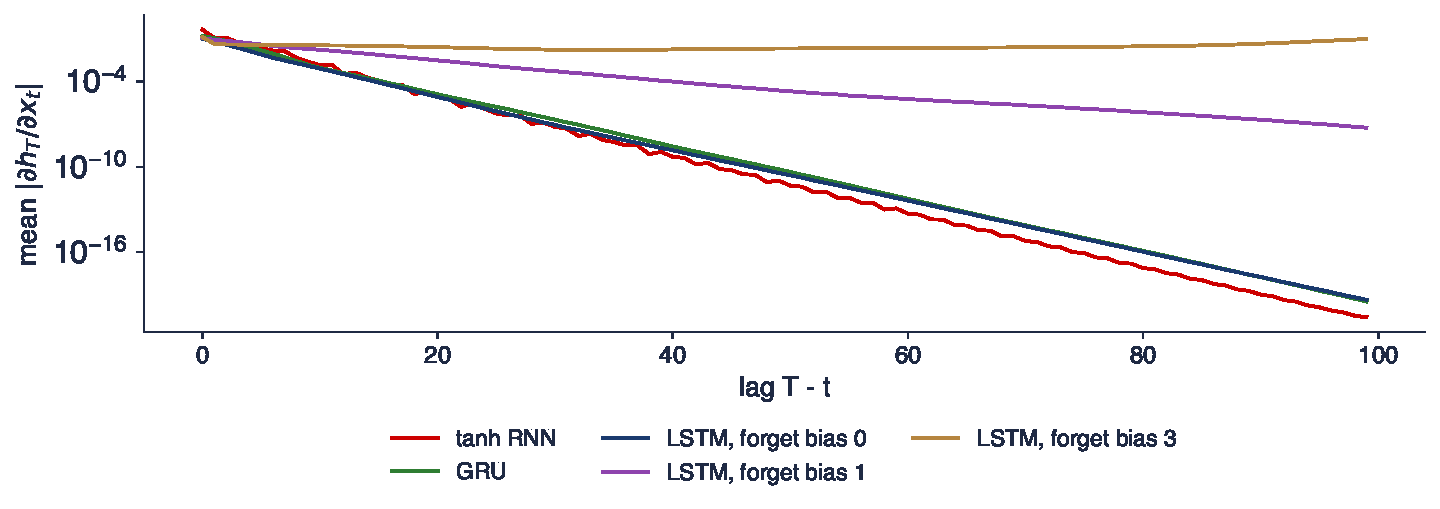
\includegraphics[width=0.97\textwidth,height=0.5\textheight,keepaspectratio]{ats_ch12_vanishing.pdf}
\end{center}
\vspace{-0.25cm}
\begin{itemize}
    \item Mean $|\partial h_T/\partial x_t|$ of freshly initialised networks (32 units, $T = 100$, Gaussian inputs, average of 5 seeds), log scale
\end{itemize}
\quantlet{ATS\_ch12\_recurrent}{\qlurl{ATS_ch12_recurrent}}
\end{frame}

\begin{frame}{Interpreting the gradients}
\itemsize{\small}
\begin{itemize}
    \item At lag 50 the gradient is a fraction $10^{-10}$ of its lag-1 value for the tanh RNN, $10^{-9}$ for the GRU and $10^{-9}$ for the LSTM with the default forget bias 0
    \item Forget bias 1: $10^{-4}$; forget bias 3: 0.47: gates help only when the forget gate is open ($\sigma(3) = 0.95$)
    \item Decay rates per lag: 0.51 (RNN), 0.45 (LSTM, bias 0), 0.03 (LSTM, bias 3): geometric in every case
    \item For daily series this matters less than it seems: HAR-type memory (22 lags) is within reach; for hourly data with weekly cycles (168 lags) it decides the architecture
\end{itemize}
\end{frame}

\begin{frame}{Temporal convolutional networks}
\itemsize{\small}
\begin{itemize}
    \item Causal dilated convolution: a weighted sum of past inputs spaced $d$ steps apart \refWaveNet
    \[ z_t = \sum_{j=0}^{k-1} w_j\,x_{t - d\,j} \]
    \begin{itemize}
        \item $k$: kernel size; $w_j$: filter weights; $d$: dilation (skips $d - 1$ steps); only the past enters (causal)
        \item TCN \refBaiK: residual blocks of two dilated causal convolutions, $d = 1, 2, 4, \dots, 2^{\ell-1}$ over $\ell$ levels
    \end{itemize}
    \item Receptive field: how far back the network can look
    \[ R = 1 + 2(k - 1)(2^\ell - 1) \]
    \begin{itemize}
        \item $k = 3$, $\ell = 4$: $R = 61$; one week of hours needs $\ell = 7$ ($R = 509$); memory is set by the architecture: no vanishing over time, but nothing beyond $R$
    \end{itemize}
    \item Parallel over time (fast training), stable gradients; Bai et al.\ found TCNs competitive with LSTMs on standard sequence tasks
\end{itemize}
\end{frame}

\begin{frame}{Multi-step forecasts and sequence-to-sequence}
\itemsize{\small}
\begin{itemize}
    \item \textbf{Recursive}: one-step model iterated, forecasts fed back as inputs: errors accumulate, the model is trained for $h = 1$ only
    \item \textbf{Direct}: one model per horizon $h$ (our HAR and network forecasts); \textbf{MIMO}: one network outputs the whole vector $(\hat y_{t+1},\dots,\hat y_{t+H})$ (DLinear, N-BEATS, Transformers here)
    \item \textbf{Encoder--decoder} \refSVL: an encoder RNN reads the past into a state, a decoder RNN unrolls the future; trained with teacher forcing
    \begin{itemize}
        \item exposure bias: at test time the decoder sees its own errors; DeepAR samples paths instead
    \end{itemize}
    \item Survey of recurrent forecasting practice \refHBB: deseasonalise or add seasonal lags, scale per series, train globally, ensemble seeds
\end{itemize}
\end{frame}

\begin{frame}{Design: deep models against HAR}
\itemsize{\small}
\begin{itemize}
    \item Target $y = \log RV$ of the S\&P 500 (\refOMI); forecasts of $RV_{t+h}$, $h \in \{1, 5, 22\}$, direct; level forecast $\exp(\hat m + s^2/2)$ with the training residual variance
    \item Expanding window, first forecast after 2500 days (24 December 2009), re-estimation every 500 days; 3\,051 forecasts per horizon
    \item Models on the last 22 values: HAR \refCor\ (OLS), MLP (2 $\times$ 32 units), LSTM (16 units), TCN (3 levels, $R = 29$), HGB on the 22 lags; one seed per network
    \item QLIKE \refPat, DM (HLN) against HAR, MCS; the literature: neural networks gain little over HAR \refBuc; ML gains appear mostly with many predictors \refCSV
\end{itemize}
\end{frame}

\begin{frame}{Can deep networks beat HAR?}
\itemsize{\footnotesize}
\begin{center}
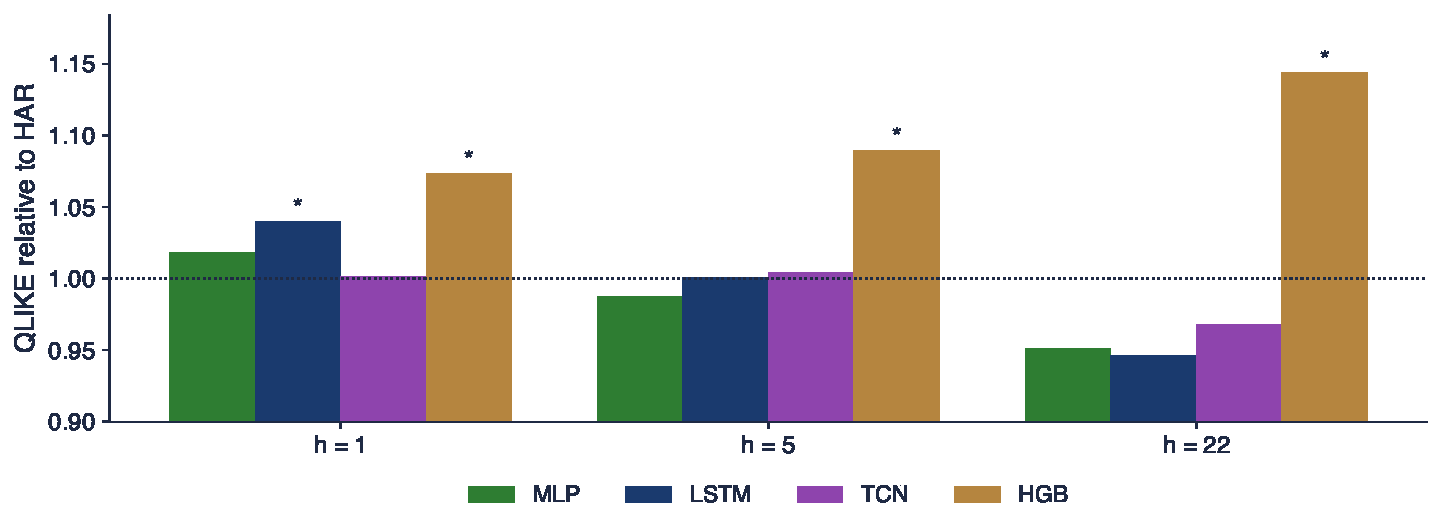
\includegraphics[width=0.97\textwidth,height=0.5\textheight,keepaspectratio]{ats_ch12_rv_deep.pdf}
\end{center}
\vspace{-0.25cm}
\begin{itemize}
    \item QLIKE relative to HAR (1 = HAR); a star marks a DM rejection at 5\%
\end{itemize}
\quantlet{ATS\_ch12\_recurrent}{\qlurl{ATS_ch12_recurrent}}
\end{frame}

\begin{frame}{Interpreting deep models against HAR}
\itemsize{\small}
\begin{itemize}
    \item $h = 1$: MLP 1.019, LSTM 1.040 (DM 2.77), TCN 1.002, HGB 1.074 (DM 3.84): nothing beats HAR, two are significantly worse
    \item $h = 22$: MLP 0.951, LSTM 0.946, TCN 0.968: gains of 3--5\% that DM does not confirm ($p$ 0.132, 0.444); HAR stays in the MCS ($p$ 0.49)
    \item Boosting on raw lags is the worst at every horizon: trees cannot extrapolate to the volatility peaks of 2020
    \item HAR is a linear model with the right three features; a network must rediscover them from a few thousand days
\end{itemize}
\end{frame}

\begin{frame}{Recap: Deep learning for sequences}
\itemsize{\small}
\begin{itemize}
    \item Gradients through time are products of Jacobians: they vanish geometrically unless the LSTM forget gate stays open
    \item TCNs fix the memory by the receptive field; multi-step forecasts are recursive, direct or MIMO
    \item On daily realised variance, networks do not significantly beat HAR at any horizon
\end{itemize}
\end{frame}


%=============================================================================
\section{Attention and Transformers}
%=============================================================================

\begin{frame}{Scaled dot-product attention}
\itemsize{\small}
\begin{itemize}
    \item \refVas: each token attends to all tokens, with weights given by query--key similarity
    \[ Q = XW_Q, \quad K = XW_K, \quad V = XW_V \]
    \[ \mathrm{Att}(Q, K, V) = \mathrm{softmax}\Big(\frac{QK'}{\sqrt{d_k}}\Big)V \]
    \begin{itemize}
        \item $X \in \mathbb R^{n\times d}$: $n$ tokens of dimension $d$; $W_Q, W_K, W_V$: learned projections to queries, keys and values; $d_k$: key dimension; softmax normalises each row to weights that sum to 1
        \item each output is a weighted average of the values, with data-dependent weights; $\sqrt{d_k}$ keeps the logits of order one; multi-head: several projections in parallel, concatenated
    \end{itemize}
    \item Permutation equivariant: without \textbf{positional encodings} the order of the tokens is lost, which is fatal for time series
    \item Cost $O(n^2 d)$ in time and memory: one token per hour and a week of input give $n = 168$; a month gives $n = 720$
    \begin{itemize}
        \item the long-horizon Transformers of 2020--2022 were mostly about this cost
    \end{itemize}
\end{itemize}
\end{frame}

\begin{frame}{Transformers for long horizons}
\itemsize{\small}
\begin{itemize}
    \item \textbf{Informer} \refInf: ProbSparse attention (only the most informative queries), self-attention distilling, a generative decoder that outputs the horizon at once: $O(n\log n)$
    \item \textbf{Autoformer} \refAuto: series decomposition inside every layer (moving-average trend and remainder) and an auto-correlation mechanism that aggregates sub-series at lags found by FFT
    \item \textbf{PatchTST} \refNie: tokens are \textbf{patches} of consecutive values (e.g.\ 16 or 24), each channel modelled separately, instance normalisation
    \begin{itemize}
        \item fewer tokens ($n/P$), local semantics in each token, longer look-backs affordable
    \end{itemize}
    \item All were evaluated on the same handful of benchmarks (electricity, traffic, weather, ETT) with MSE on standardised data
\end{itemize}
\end{frame}

\begin{frame}{Are Transformers effective? The Zeng et al.\ (2023) critique}
\itemsize{\small}
\begin{itemize}
    \item \refZeng: self-attention is permutation-invariant; point-wise tokens carry no local semantics; positional encodings only partly restore order
    \item LTSF-Linear baselines: one linear map from the last $L$ values to the next $H$
    \[ \textbf{Linear:}\ \hat y_{t+1:t+H} = W\,x_{t-L+1:t} \]
    \[ \textbf{DLinear:}\ \hat y = \big(W_s(I - A) + W_tA\big)\,x \]
    \begin{itemize}
        \item $W$: an $H \times L$ weight matrix; \textbf{NLinear} subtracts and adds back the last value; \textbf{DLinear}: $A$ the moving-average matrix, $W_t$ for the trend $Ax$, $W_s$ for the remainder (Seminar 12, A8)
    \end{itemize}
    \item Their finding: these one-layer models beat Informer, Autoformer and their successors on most of the standard long-horizon benchmarks
    \begin{itemize}
        \item and the Transformers did not improve with a longer look-back $L$: a sign they did not use the extra history
    \end{itemize}
    \item PatchTST was the reply: patching and channel independence put Transformers back ahead of DLinear on the same benchmarks
\end{itemize}
\end{frame}

\begin{frame}{Replication design: the Zeng et al.\ protocol on Romanian load}
\itemsize{\small}
\begin{itemize}
    \item Hourly Romanian load as one series ($n = 32\,856$ hours), z-scored with training moments; chronological split 7:1:2; test from 31 December 2025
    \item Look-back $L = 336$ hours; horizons $H = 96$ and $336$; MSE and MAE on the z-scored series, as in their tables
    \item Models: repeat the last value, seasonal naive (last week), Linear, NLinear, DLinear (kernel 25), a patch Transformer (14 patches of 24 hours, 1 layer, 4 heads) and the same Transformer with one token per hour
    \item Adam, MSE, early stopping on the validation block; three seeds averaged (one for the point-token Transformer, whose cost is $O(n^2)$)
\end{itemize}
\end{frame}

\begin{frame}{Linear models, Transformers and the role of tokens}
\itemsize{\footnotesize}
\begin{center}
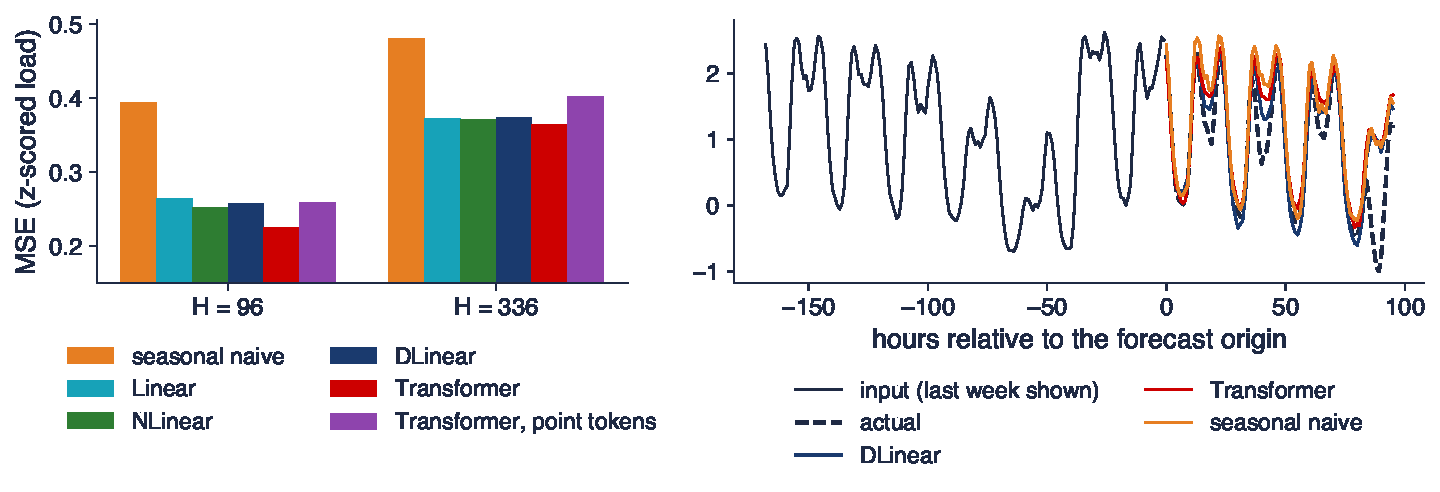
\includegraphics[width=0.97\textwidth,height=0.48\textheight,keepaspectratio]{ats_ch12_zeng.pdf}
\end{center}
\vspace{-0.25cm}
\begin{itemize}
    \item Left: test MSE by horizon (repeating the last value, 1.585 and 1.699, is off the scale); right: one test window at $H = 96$ (the last week of input, the actual load and three forecasts)
\end{itemize}
\quantlet{ATS\_ch12\_transformers}{\qlurl{ATS_ch12_transformers}}
\end{frame}

\begin{frame}{Interpreting the protocol}
\itemsize{\small}
\begin{itemize}
    \item $H = 96$: seasonal naive 0.393, Linear 0.265, NLinear 0.253, DLinear 0.257; point-token Transformer 0.258; patch Transformer 0.226
    \item $H = 336$: DLinear 0.374, point tokens 0.402 (worse than every linear model), patches 0.364
    \item Both papers replicate on our data: the point-token Transformer is no better than NLinear or DLinear at $H = 96$ and worse than every linear model at $H = 336$; patching overturns the ranking
    \item The gap between the best linear model and the patch Transformer shrinks from 0.253 against 0.226 at $H = 96$ to 0.371 against 0.364 at $H = 336$: at long horizons the series is mostly seasonal level
\end{itemize}
\end{frame}

\begin{frame}{The Temporal Fusion Transformer}
\itemsize{\small}
\begin{itemize}
    \item \refTFT: built for multi-horizon forecasts with three kinds of inputs: static (the store, the country), known future (calendar, prices), observed past
    \item Components
    \begin{itemize}
        \item gated residual networks (GRN): $\mathrm{LayerNorm}\big(a + \mathrm{GLU}(\eta)\big)$, a gate that can switch a block off
        \item variable selection networks: softmax weights over the inputs at each time
        \item static covariate encoders that condition every other block; an LSTM encoder--decoder for local patterns
        \item interpretable multi-head attention (values shared across heads) for long-range dependence; quantile outputs trained with the pinball loss
    \end{itemize}
    \item Its ``interpretability'' is the variable-selection weights and the attention pattern: useful diagnostics, not causal explanations (Section 7)
\end{itemize}
\end{frame}

\begin{frame}{Recap: Attention and Transformers}
\itemsize{\small}
\begin{itemize}
    \item Attention is a data-dependent weighted average; order comes only from positional encodings; cost is quadratic in the tokens
    \item Zeng et al.: one linear layer beat point-token Transformers; PatchTST: patches restore the advantage; both replicate on Romanian load
    \item The TFT organises static, known and observed inputs with gates, selection and attention, and outputs quantiles
\end{itemize}
\end{frame}


%=============================================================================
\section{Global deep models: N-BEATS, N-HiTS, DeepAR}
%=============================================================================

\begin{frame}{N-BEATS: basis expansion with residual stacking}
\itemsize{\small}
\begin{itemize}
    \item \refOre: each block reconstructs part of its input (backcast) and forecasts the rest
    \[ \hat x_\ell = g^b(\theta^b_\ell), \quad \hat y_\ell = g^f(\theta^f_\ell) \]
    \[ x_{\ell+1} = x_\ell - \hat x_\ell, \quad \hat y = \sum_\ell\hat y_\ell \]
    \begin{itemize}
        \item $x_\ell$: input of block $\ell$; $\theta^b_\ell, \theta^f_\ell$: coefficients produced by four fully connected layers; $g^b$, $g^f$: basis functions; doubly residual: each block explains what the previous ones left
    \end{itemize}
    \item \textbf{Generic}: $g$ linear and learned; \textbf{interpretable}: trend basis $\{(t/H)^j\}_{j\le3}$ and seasonality basis $\{\cos 2\pi jt/H, \sin 2\pi jt/H\}$
    \begin{itemize}
        \item $H$: forecast horizon; a learned decomposition, similar to exponential smoothing
    \end{itemize}
    \item Pure deep learning, no time-series features; trained globally per frequency with sMAPE/MASE losses; the published results are ensembles of 180 networks
    \begin{itemize}
        \item their M4 result beat the competition winner, the ES-RNN hybrid of \refSmyl
    \end{itemize}
\end{itemize}
\end{frame}

\begin{frame}{N-HiTS: multi-rate inputs, hierarchical outputs}
\itemsize{\small}
\begin{itemize}
    \item \refNHiTS: block $\ell$ first max-pools its input with kernel $k_\ell$ (e.g.\ 8, 4, 1): low-resolution blocks see the long-run shape, high-resolution blocks the detail
    \item Each block outputs only $H/r_\ell$ coefficients, interpolated to $H$ points: the expressiveness ratio $r_\ell$ forces coarse blocks to forecast smooth components
    \begin{itemize}
        \item an explicit frequency decomposition of the forecast, close in spirit to the wavelet multiresolution of \atschlink{https://danpele.github.io/Advanced-Time-Series/EN/Courses/chapter11_spectral_wavelet_analysis.pdf}{Chapter 11}
    \end{itemize}
    \item Fewer parameters and less compute than N-BEATS for long horizons, with similar accuracy on short ones
    \item Ours: generic N-BEATS (3 blocks $\times$ 3 layers $\times$ 256 units) and N-HiTS (pools 8, 4, 1), input 336 hours, each window divided by its mean absolute level, MAE loss, median of 3 seeds
\end{itemize}
\end{frame}

\begin{frame}{Design: the M4 hourly subset}
\itemsize{\small}
\begin{itemize}
    \item \refMfourA: 414 hourly series, horizon 48
    \item Accuracy measures: symmetric MAPE, scaled error and their average relative to Naive 2
    \[ \mathrm{OWA} = \frac12\Big(\frac{\mathrm{sMAPE}}{\mathrm{sMAPE}_{\mathrm{Naive2}}} + \frac{\mathrm{MASE}}{\mathrm{MASE}_{\mathrm{Naive2}}}\Big) \]
    \begin{itemize}
        \item sMAPE: mean of $2|y - \hat y|/(|y| + |\hat y|)$ in \%; MASE: mean absolute error divided by the in-sample MAE of the seasonal naive (period 24) \refHK; OWA $< 1$: better than Naive 2
    \end{itemize}
    \item Our Naive, seasonal naive and Naive 2 reproduce the official M4 evaluation file exactly: Naive 2 sMAPE 18.38 (official 18.38), MASE 2.40 (official 2.40)
    \item Reference points from the same file: the M4 MLP and RNN benchmarks (OWA 0.921 and 1.036), Theta 1.006, the winner \refSmyl\ 0.440, the runner-up Montero-Manso et al.\ 0.484; all global models are trained only on the training parts
\end{itemize}
\end{frame}

\begin{frame}{Global deep models on the M4 hourly series}
\itemsize{\footnotesize}
\begin{center}
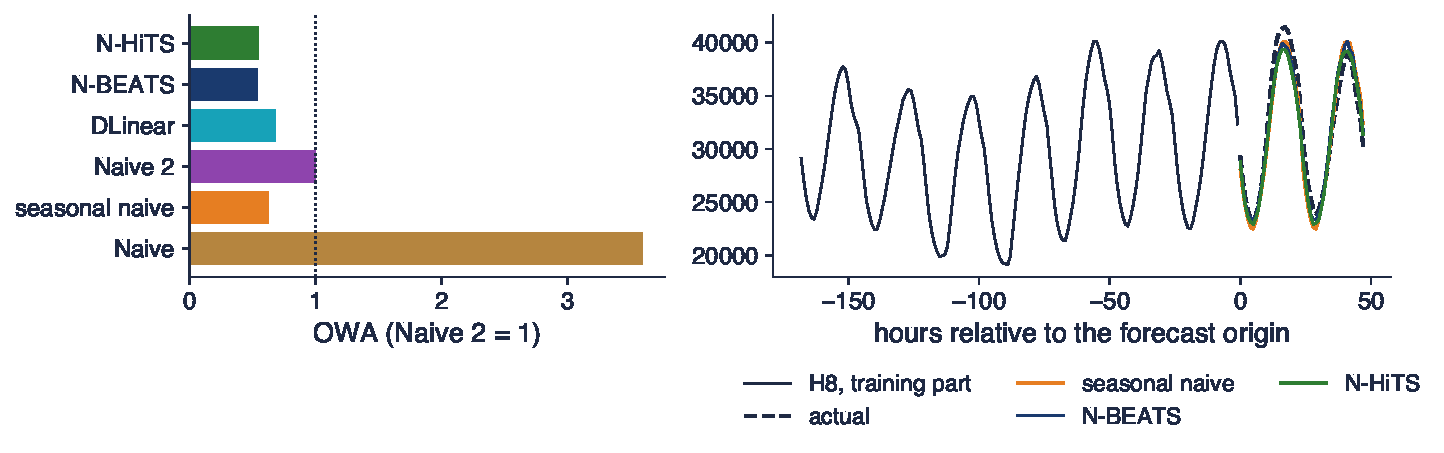
\includegraphics[width=0.97\textwidth,height=0.48\textheight,keepaspectratio]{ats_ch12_m4.pdf}
\end{center}
\vspace{-0.25cm}
\begin{itemize}
    \item Left: OWA (Naive 2 = 1); right: one series with the seasonal naive, N-BEATS and N-HiTS forecasts
\end{itemize}
\quantlet{ATS\_ch12\_global\_deep}{\qlurl{ATS_ch12_global_deep}}
\end{frame}

\begin{frame}{Interpreting the M4 hourly results}
\itemsize{\small}
\begin{itemize}
    \item OWA: seasonal naive 0.628, DLinear 0.683, N-BEATS 0.539 (sMAPE 10.73, MASE 1.19), N-HiTS 0.548
    \item A few minutes of CPU training put N-BEATS ahead of every M4 benchmark and of the M4 neural benchmarks (0.921, 1.036), behind the two best entries (0.440, 0.484)
    \item The M4 neural benchmarks were local (one network per series); ours are global: pooling 414 series is what makes the difference
    \item DLinear is weaker here: hourly M4 series need nonlinear interactions of level and season that one linear layer cannot express
\end{itemize}
\end{frame}

\begin{frame}{DeepAR: probabilistic forecasts from a global RNN}
\itemsize{\small}
\begin{itemize}
    \item \refDeepAR: an LSTM state per series drives the parameters of a likelihood
    \[ h_{i,t} = \mathrm{LSTM}(h_{i,t-1}, z_{i,t-1}, x_{i,t}), \qquad z_{i,t} \sim \ell\big(\cdot\mid\theta(h_{i,t})\big) \]
    \begin{itemize}
        \item $z_{i,t}$: value of series $i$ at $t$; $x_{i,t}$: covariates (lags at 1, 24, 168, calendar); $\theta(h)$: e.g.\ Gaussian $(\mu, \sigma)$ for real data, negative binomial for counts
        \item training: maximise $\sum_{i,t}\log\ell(z_{i,t}\mid\theta(h_{i,t}))$ over random windows of all series, each scaled by $1 + $ the mean of its context
    \end{itemize}
    \item Forecast: ancestral sampling, each draw fed back as the next input; quantiles from the sample paths
    \[ \mathrm{wQL} = \sum_\tau\frac{2\sum_{i,t}\rho_\tau(z_{i,t} - \hat q_{\tau,i,t})}{\sum_{i,t}|z_{i,t}|} \]
    \begin{itemize}
        \item weighted quantile loss: $\rho_\tau$ the pinball loss at level $\tau$, $\hat q_\tau$ the forecast quantile; an approximation of the CRPS \refGR, lower is better
    \end{itemize}
    \item The model of choice for large retail and energy panels; the base of several foundation models (\atschlink{https://danpele.github.io/Advanced-Time-Series/EN/Courses/chapter13_foundation_models_conformal.pdf}{Chapter 13})
\end{itemize}
\end{frame}

\begin{frame}{A small DeepAR on the M4 hourly series}
\itemsize{\footnotesize}
\begin{center}
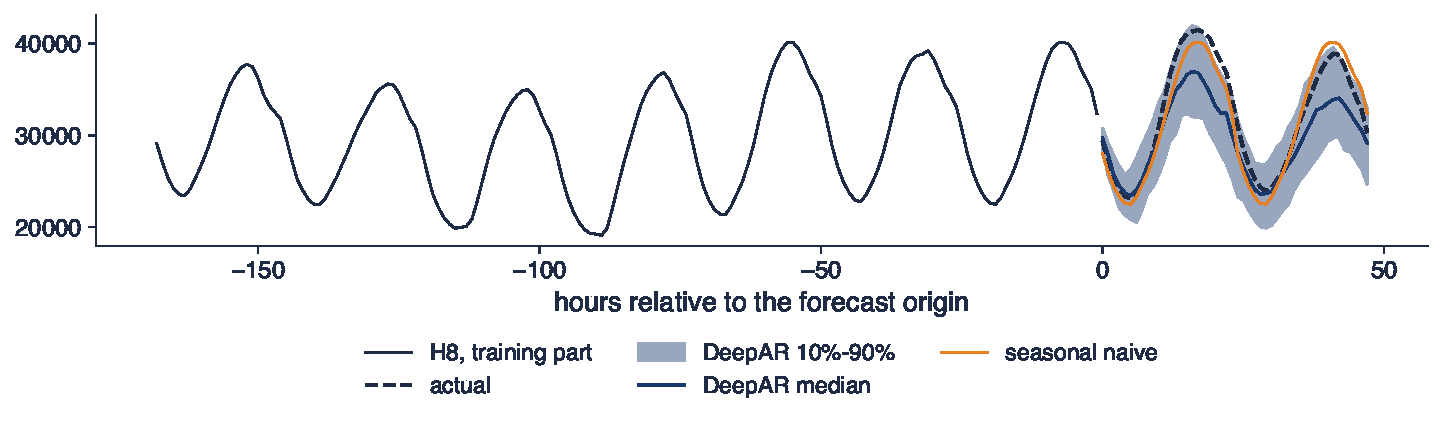
\includegraphics[width=0.97\textwidth,height=0.46\textheight,keepaspectratio]{ats_ch12_deepar.pdf}
\end{center}
\vspace{-0.25cm}
\begin{itemize}
    \item Two-layer LSTM (40 units), context 168 hours, 4\,000 training steps of 64 windows, 100 sample paths; the same series as on the previous chart
\end{itemize}
\quantlet{ATS\_ch12\_global\_deep}{\qlurl{ATS_ch12_global_deep}}
\end{frame}

\begin{frame}{Interpreting DeepAR}
\itemsize{\small}
\begin{itemize}
    \item wQL by training budget (steps): 500: 0.0344, 1000: 0.0338, 2000: 0.0374, 4000: 0.0405; seasonal naive with empirical quantiles: 0.0375
    \item After 1000 steps DeepAR beats the benchmark (80\% coverage 83\%); with longer training it overfits the training windows and loses (76\% at 4000 steps)
    \item Choosing the best checkpoint on this table would be data snooping: the budget must be fixed on a validation block before the test period is opened
    \item Probabilistic deep models are sensitive to the training budget; report the rule that set it, and the benchmark under a proper score
\end{itemize}
\end{frame}

\begin{frame}{Lessons from the M5 competition}
\itemsize{\small}
\begin{itemize}
    \item \refMfiveA: 42\,840 Walmart series in a hierarchy, daily unit sales, 28 days ahead; accuracy and uncertainty tracks
    \begin{itemize}
        \item the winning accuracy methods were global LightGBM models on engineered features (lags, rolling means, prices, calendar), often combined
    \end{itemize}
    \item Global models, cross-learning and external information (prices, events) mattered more than architecture
    \item The simple benchmarks were beaten, but by smaller margins than ML marketing suggests, and least at the bottom level of the hierarchy
    \item An earlier warning: ML methods lost to statistical ones on the M3 monthly data \refMSAa; the difference between M3 and M5 is data size and cross-series learning
\end{itemize}
\end{frame}

\begin{frame}{Recap: Global deep models}
\itemsize{\small}
\begin{itemize}
    \item N-BEATS and N-HiTS: residual stacks of fully connected blocks, generic or with trend and seasonal bases, multi-rate in N-HiTS
    \item On M4 hourly, global N-BEATS beats every benchmark and the local neural networks of M4
    \item DeepAR gives sample paths from a likelihood; it beats the seasonal naive under the wQL only at the right training budget, which must be set on validation data
\end{itemize}
\end{frame}


%=============================================================================
\section{Interpretation and the honest benchmark}
%=============================================================================

\begin{frame}{Shapley values (1/2): the definition}
\itemsize{\small}
\begin{itemize}
    \item \refSha: the fair share of player $g$ in a cooperative game $v$ with $G$ players
    \[ \phi_g = \sum_{S \subseteq \{1..G\}\setminus g}\frac{|S|!\,(G - |S| - 1)!}{G!}\big[v(S\cup g) - v(S)\big] \]
    \begin{itemize}
        \item $v(S)$: the value of coalition $S$; $v(S\cup g) - v(S)$: the marginal contribution of $g$; the weights average it over all orders in which players can join
    \end{itemize}
    \item The unique allocation with four axioms
    \begin{itemize}
        \item efficiency ($\sum_g\phi_g = v(\mathrm{all}) - v(\emptyset)$), symmetry, dummy (a player who adds nothing gets 0) and additivity
    \end{itemize}
\end{itemize}
\end{frame}

\begin{frame}{Shapley values (2/2): SHAP for forecasts}
\itemsize{\small}
\begin{itemize}
    \item SHAP \refLL: players are features; the value of a coalition $S$ is the expected forecast when only $x_S$ is known
    \[ v(S) = \E\big[f(x_S, X_{\bar S})\big] \]
    \begin{itemize}
        \item $f$: the fitted model; $\bar S$: the other features; \textbf{interventional}: $X_{\bar S}$ from a background sample, independent of $x_S$; \textbf{observational}: conditional on $x_S$
        \item with lags, features are strongly correlated: interventional values evaluate the model at impossible histories; group correlated lags instead
    \end{itemize}
    \item Here: exact Shapley values of three lag groups (day, days 2--5, days 6--22) for boosting on S\&P 500 log RV, 300 forecast days, 100 background days
\end{itemize}
\end{frame}

\begin{frame}{What the boosted model has learned}
\itemsize{\footnotesize}
\begin{center}
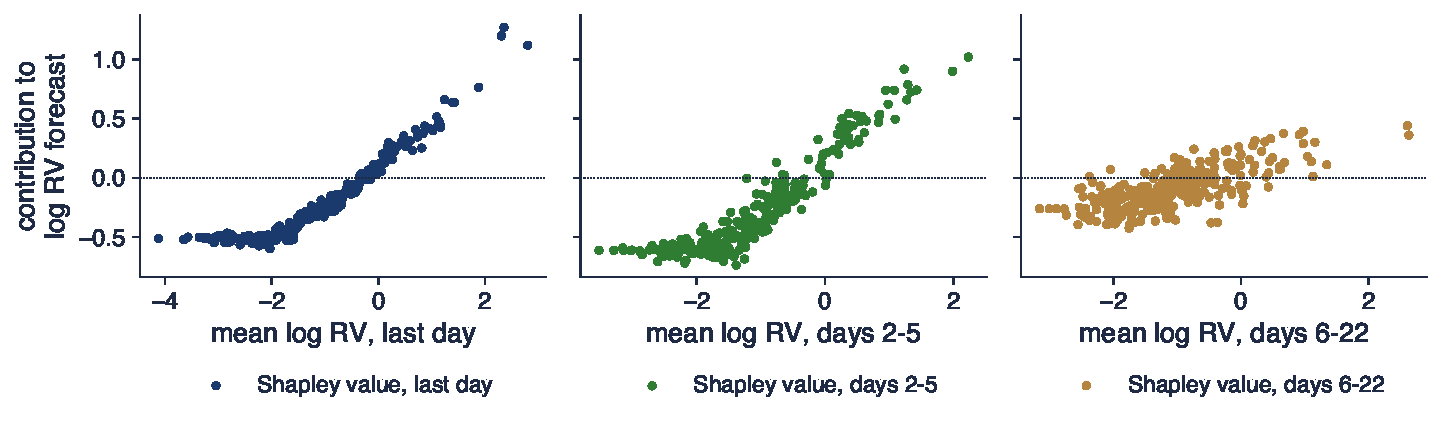
\includegraphics[width=0.97\textwidth,height=0.44\textheight,keepaspectratio]{ats_ch12_shap.pdf}
\end{center}
\vspace{-0.25cm}
\begin{itemize}
    \item Each point: one forecast day; horizontal: the mean log RV of the group; vertical: its Shapley value
\end{itemize}
\quantlet{ATS\_ch12\_interpretation}{\qlurl{ATS_ch12_interpretation}}
\end{frame}

\begin{frame}{Interpreting the Shapley values}
\itemsize{\small}
\begin{itemize}
    \item Mean $|\phi|$ shares: last day 37\%, days 2--5 46\%, days 6--22 17\%
    \item HAR on the same sample: coefficients 0.28, 0.50, 0.17 on the daily, weekly and monthly means: the boosted trees rediscovered the HAR cascade
    \item The values flatten at the extremes: trees cap their forecasts at the training range, the reason boosting lost to HAR in 2020
    \item Shapley values describe the model, not the data-generating process: a correct description of a wrong model is still wrong
\end{itemize}
\end{frame}

\begin{frame}{Attention is not explanation}
\itemsize{\small}
\begin{itemize}
    \item \refJW: attention weights are often uncorrelated with gradient-based importance, and very different attention patterns give the same predictions
    \item \refWP: attention can be a faithful explanation under conditions, but this must be tested, not assumed
    \item A test: occlusion importance, the increase of the MSE when one input patch is replaced by the window mean, against the attention each patch receives
    \begin{itemize}
        \item on the patch Transformer of Section 5 ($H = 96$), the first 1000 test windows
    \end{itemize}
\end{itemize}
\end{frame}

\begin{frame}{Where the Transformer looks, and what it uses}
\itemsize{\footnotesize}
\begin{center}
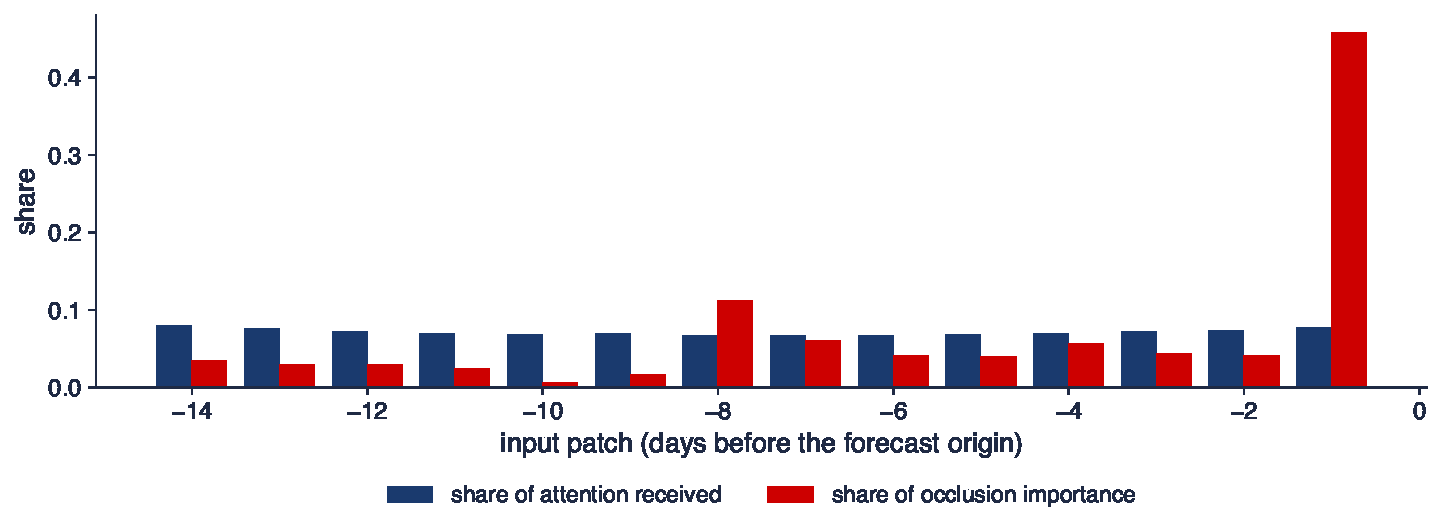
\includegraphics[width=0.97\textwidth,height=0.46\textheight,keepaspectratio]{ats_ch12_attention.pdf}
\end{center}
\vspace{-0.25cm}
\begin{itemize}
    \item Share of attention received by each of the 14 daily patches against the share of occlusion importance
\end{itemize}
\quantlet{ATS\_ch12\_interpretation}{\qlurl{ATS_ch12_interpretation}}
\end{frame}

\begin{frame}{Interpreting attention and occlusion}
\itemsize{\small}
\begin{itemize}
    \item The last day carries 46\% of the occlusion importance but receives only 8\% of the attention
    \item Most attention goes to the patch 14 days back; the most important patch is 1 day back; Spearman correlation \ensuremath{-}0.09
    \item The flatten head reads the token states directly: what matters can bypass the attention weights entirely
    \item Report attention maps as what they are, a mixing pattern; for importance, use occlusion, Shapley or gradients, with a sanity check
\end{itemize}
\end{frame}

\begin{frame}{The honest benchmark}
\itemsize{\small}
\begin{itemize}
    \item Strong baselines first: seasonal naive, ETS/Theta, HAR, an expert ARX; Lago et al.\ built an open benchmark because published electricity-price models were rarely compared with them \refLMDW
    \item Pitfalls catalogued by \refHAB: test-set reuse, leakage in scaling and features, errors averaged across series of different scales, no significance tests, unreported tuning budget
    \item Tests (\atschlink{https://danpele.github.io/Advanced-Time-Series/EN/Courses/chapter1_forecast_evaluation.pdf}{Chapter 1}): DM for two models, MCS \refHLN\ for many, the reality check \refWhi\ and SPA \refHan\ when the best of many was chosen on the same data
    \item Report seeds, hardware, training time, every architecture tried; pre-register the design (\atschlink{https://danpele.github.io/Advanced-Time-Series/EN/Courses/chapter0_refresher_inference.pdf}{Chapter 0})
\end{itemize}
\end{frame}

\begin{frame}{Seeds and data snooping}
\itemsize{\footnotesize}
\begin{center}
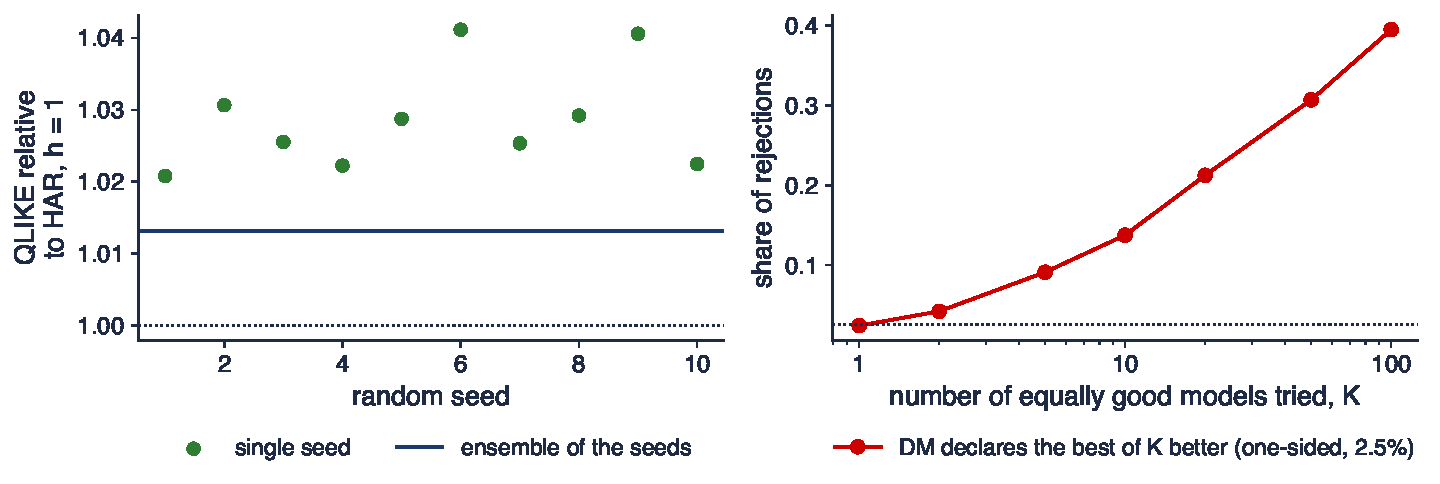
\includegraphics[width=0.97\textwidth,height=0.46\textheight,keepaspectratio]{ats_ch12_snooping.pdf}
\end{center}
\vspace{-0.25cm}
\begin{itemize}
    \item Left: MLP against HAR for S\&P 500 RV, $h = 1$, with 10 seeds and their ensemble; right: simulation, $K$ equally good models, 2500 test days, correlation 0.5
\end{itemize}
\quantlet{ATS\_ch12\_interpretation}{\qlurl{ATS_ch12_interpretation}}
\end{frame}

\begin{frame}{Interpreting seeds and snooping}
\itemsize{\small}
\begin{itemize}
    \item Seeds alone move the QLIKE ratio from 1.019 to 1.041 (median 1.027); the ensemble of the seeds reaches 1.013, better than every single seed
    \item Picking the best of $K$ equally good models on the test set: the DM test declares it better (one-sided, nominal 2.5\%) in 2\% of cases for $K = 1$, 14\% for $K = 10$, 40\% for $K = 100$
    \item Hyper-parameter searches, seeds and architectures are all $K$: count them, and test the winner with SPA or MCS on data not used for the choice
    \item Ensembles are the cheap cure for seed variance; pre-registration is the cure for snooping
\end{itemize}
\end{frame}

\begin{frame}{Recap: Interpretation and honest benchmarks}
\itemsize{\small}
\begin{itemize}
    \item Shapley values have axioms; with lagged features use groups and remember they describe the model
    \item Attention weights are not importance: on our Transformer they point the other way
    \item Strong baselines, DM/MCS/SPA, all seeds and all tries reported: otherwise any model can be made to win
\end{itemize}
\end{frame}


%=============================================================================
\section{AI for scientific discovery}
%=============================================================================

\begin{frame}{An open question}
\itemsize{\small}
\begin{itemize}
    \item Do machine-learning and deep models forecast realised volatility better than HAR, across markets and horizons, once the comparison is pre-registered?
    \begin{itemize}
        \item formal: $H_0$: $\E[\mathrm{QLIKE}_{\mathrm{ML}} - \mathrm{QLIKE}_{\mathrm{HAR}}] \ge 0$ in each cell; a cell supports ML only if DM rejects at 5\% and the MCS excludes HAR
        \item falsified if fewer than a fifth of the cells support ML
    \end{itemize}
    \item Why it matters: risk systems (VaR, margins, option hedging) run on volatility forecasts; a spurious ML gain becomes a model risk
    \begin{itemize}
        \item literature to start from: \refCor, \refBuc, \refCSV, \refHAB
    \end{itemize}
\end{itemize}
\end{frame}

\begin{frame}{The discovery loop with an AI assistant}
\itemsize{\footnotesize}
\begin{itemize}
    \item An AI assistant (an LLM such as Claude, ChatGPT, Gemini or Copilot) speeds up each step; Semantic Scholar and Elicit help with the literature
    \begin{itemize}
        \item \textbf{literature}: \aiprompt{List peer-reviewed papers since 2019 comparing neural networks or boosting with HAR for realised volatility out of sample; give DOIs and the test used.} Then check every DOI on Crossref
        \item \textbf{design}: \aiprompt{Write a pre-registration: assets, horizons, windows, refit schedule, loss, tests, seeds, what counts as a win.}
        \item \textbf{code and replication}: reproduce first the S\&P 500 HAR QLIKE (0.253 at $h = 1$ here), then add learners one at a time
        \item \textbf{critique}: \aiprompt{Act as a hostile referee: list every source of leakage, snooping and unfair tuning in this comparison.}
    \end{itemize}
    \item Report: what was asked, what was kept, what was rejected (AI\_USE.md, AI\_ERRORS.md)
\end{itemize}
\end{frame}

\begin{frame}{What the human checks}
\itemsize{\small}
\begin{itemize}
    \item Every reference exists and says what is claimed (DOI resolves, title matches, the result is in the paper)
    \item No future information: scaling, feature construction and tuning use only data before each origin; purge around $h$-step targets
    \item The baseline is tuned as carefully as the learner, and refitted on the same schedule
    \item Seeds, architectures and hyper-parameters tried are all reported; the winner is tested with MCS or SPA
    \item An AI claim that ``LSTMs capture long memory, so they beat HAR'' is checked against the numbers, not accepted
\end{itemize}
\end{frame}

\begin{frame}{Mini-case: do learners beat HAR across markets?}
\itemsize{\footnotesize}
\begin{center}
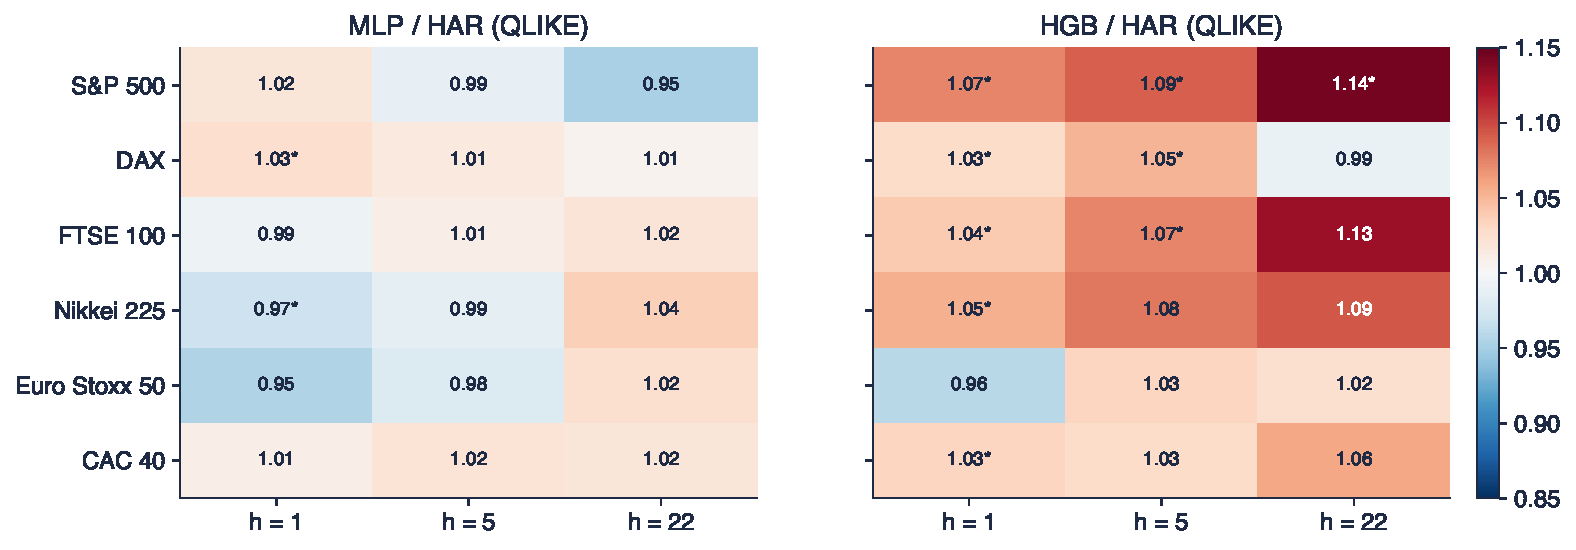
\includegraphics[width=0.97\textwidth,height=0.44\textheight,keepaspectratio]{ats_ch12_ai_case.pdf}
\end{center}
\vspace{-0.25cm}
\begin{itemize}
    \item 36 cells: six indices $\times$ three horizons $\times$ two learners (MLP, boosting), the expanding design of Section 4; QLIKE ratio to HAR, a star where DM rejects at 5\%
    \item Ratios from 0.95 to 1.14, median 1.024 (MLP 1.009, boosting 1.052); 9 cells below 1, 1 significantly better, 10 significantly worse: the hypothesis is falsified for these learners
\end{itemize}
\quantlet{ATS\_ch12\_ai\_case}{\qlurl{ATS_ch12_ai_case}}
\end{frame}

\begin{frame}{Project idea}
\itemsize{\small}
\begin{itemize}
    \item \textbf{Deep learning against HAR for Central and Eastern European volatility}: replicate first, then extend
    \begin{itemize}
        \item replicate: \refCor\ HAR and the neural comparison of \refBuc\ on the Oxford-Man indices, with the design of Section 4
        \item extend: intraday-based RV for the BET, WIG20 and EUR/RON; global models across markets; exogenous predictors (VIX, macro news) as in \refCSV
        \item pre-register: markets, horizons, windows, every learner and its tuning budget, QLIKE, DM, MCS, seeds
    \end{itemize}
    \item Deliverables follow the course rules: repository, report, AI\_USE.md, AI\_ERRORS.md, oral defence
\end{itemize}
\end{frame}


%=============================================================================
\section{Wrap-up}
%=============================================================================

\begin{frame}{Key takeaways}
\itemsize{\small}
\begin{itemize}
    \item Validation must respect dependence: K-fold only for well-specified autoregressions; otherwise block, purge and keep a final test period
    \item Global models pool series and afford memory; high-dimensional selection on short macro samples is unstable
    \item Trees and networks rarely beat strong structured baselines alone (expert ARX, HAR); they help in combinations and in large panels
    \item Architecture details matter: open forget gates, patches instead of point tokens, global training
    \item Attention is not explanation; seeds and searches are hidden multiple testing
\end{itemize}
\end{frame}

\begin{frame}{Self-assessment}
\itemsize{\small}
\begin{columns}[T]
\begin{column}{0.58\textwidth}
\begin{block}{Questions}
\begin{itemize}
    \item Why is random K-fold valid for an AR(3) fitted to AR(3) data but not for 22-day targets?
    \item Which condition does the adaptive lasso remove, and how?
    \item Why does adding trees not reduce the variance of a forest below $\rho\sigma^2$?
    \item What is the receptive field of a TCN with $k = 3$ and five levels?
    \item Why can a patch Transformer beat DLinear when a point-token Transformer cannot?
\end{itemize}
\end{block}
\end{column}
\begin{column}{0.38\textwidth}
\begin{block}{Next: \atschlink{https://danpele.github.io/Advanced-Time-Series/EN/Courses/chapter13_foundation_models_conformal.pdf}{Chapter 13}}
\begin{itemize}
    \item Foundation models and conformal prediction
    \item pretrained models used zero-shot, and distribution-free intervals for any forecaster, including the ones of this chapter
\end{itemize}
\end{block}
\end{column}
\end{columns}
\end{frame}


%=============================================================================
\section{Appendix}
%=============================================================================

\begin{frame}{Appendix: the bias of K-fold under autocorrelated errors}
\itemsize{\small}
\begin{itemize}
    \item Linear model $y = X\beta + \varepsilon$; leave out row $i$: $e_{(i)} = e_i/(1 - h_{ii})$, $h_{ii}$ the leverage
    \item $\E\,e_{(i)}^2 \approx \sigma^2(1 + h_{ii}) - 2\sum_{j\ne i}\frac{H_{ij}}{1 - h_{ii}}\Cov(\varepsilon_i, \varepsilon_j)$ to first order
    \item Uncorrelated errors: the second term vanishes and LOOCV estimates the out-of-sample MSE $\sigma^2(1 + h)$: the Bergmeir--Hyndman--Koo case
    \item Positive correlation between the left-out error and the neighbouring training errors ($H_{ij} > 0$ for neighbours with similar lags): the estimate is too small; purging sets the neighbouring terms to zero
\end{itemize}
\end{frame}

\begin{frame}{Appendix: soft thresholding and the elastic net}
\itemsize{\small}
\begin{itemize}
    \item With $X'X = nI$ the objective separates: $\frac12(\beta_j - z_j)^2 + \lambda|\beta_j|$ for each $j$, $z_j = x_j'y/n$
    \item Subgradient: $0 \in \beta_j - z_j + \lambda\,\partial|\beta_j|$; if $|z_j| \le \lambda$, $\beta_j = 0$; otherwise $\beta_j = z_j - \lambda\,\mathrm{sign}(z_j)$
    \item Elastic net: $\frac12(\beta_j - z_j)^2 + \lambda\alpha|\beta_j| + \frac{\lambda(1 - \alpha)}2\beta_j^2$ gives $\beta_j = S(z_j, \lambda\alpha)/(1 + \lambda(1 - \alpha))$
    \item Adaptive lasso: threshold $\lambda w_j = \lambda/|\tilde\beta_j|^\gamma$, small for large $|\tilde\beta_j|$: the bias on large coefficients vanishes, which gives the oracle property
\end{itemize}
\end{frame}


%=============================================================================
\section{References}
%=============================================================================

\begin{frame}{References (1/6)}
\itemsize{\tiny}
\begin{itemize}
    \item Bai, S., Kolter, J. Z., \& Koltun, V. (2018). An empirical evaluation of generic convolutional and recurrent networks for sequence modeling. arXiv:1803.01271. \href{https://arxiv.org/abs/1803.01271}{arxiv.org}
    \item Basu, S., \& Michailidis, G. (2015). Regularized estimation in sparse high-dimensional time series models. \textit{The Annals of Statistics}, 43(4), 1535--1567. \href{https://doi.org/10.1214/15-AOS1315}{doi:10.1214/15-AOS1315}
    \item Belloni, A., Chernozhukov, V., \& Hansen, C. (2014). Inference on treatment effects after selection among high-dimensional controls. \textit{The Review of Economic Studies}, 81(2), 608--650. \href{https://doi.org/10.1093/restud/rdt044}{doi:10.1093/restud/rdt044}
    \item Bengio, Y., Simard, P., \& Frasconi, P. (1994). Learning long-term dependencies with gradient descent is difficult. \textit{IEEE Transactions on Neural Networks}, 5(2), 157--166. \href{https://doi.org/10.1109/72.279181}{doi:10.1109/72.279181}
    \item Benidis, K., Rangapuram, S. S., Flunkert, V., Wang, Y., et al.\ (2022). Deep learning for time series forecasting: Tutorial and literature survey. \textit{ACM Computing Surveys}, 55(6), 1--36. \href{https://doi.org/10.1145/3533382}{doi:10.1145/3533382}
    \item Bergmeir, C., \& Benítez, J. M. (2012). On the use of cross-validation for time series predictor evaluation. \textit{Information Sciences}, 191, 192--213. \href{https://doi.org/10.1016/j.ins.2011.12.028}{doi:10.1016/j.ins.2011.12.028}
    \item Bergmeir, C., Hyndman, R. J., \& Koo, B. (2018). A note on the validity of cross-validation for evaluating autoregressive time series prediction. \textit{Computational Statistics \& Data Analysis}, 120, 70--83. \href{https://doi.org/10.1016/j.csda.2017.11.003}{doi:10.1016/j.csda.2017.11.003}
    \item Berk, R., Brown, L., Buja, A., Zhang, K., \& Zhao, L. (2013). Valid post-selection inference. \textit{The Annals of Statistics}, 41(2), 802--837. \href{https://doi.org/10.1214/12-AOS1077}{doi:10.1214/12-AOS1077}
    \item Breiman, L. (1996). Bagging predictors. \textit{Machine Learning}, 24(2), 123--140. \href{https://doi.org/10.1007/BF00058655}{doi:10.1007/BF00058655}
    \item Breiman, L. (2001). Random forests. \textit{Machine Learning}, 45(1), 5--32. \href{https://doi.org/10.1023/A:1010933404324}{doi:10.1023/A:1010933404324}
    \item Bucci, A. (2020). Realized volatility forecasting with neural networks. \textit{Journal of Financial Econometrics}, 18(3), 502--531. \href{https://doi.org/10.1093/jjfinec/nbaa008}{doi:10.1093/jjfinec/nbaa008}
    \item Burman, P., Chow, E., \& Nolan, D. (1994). A cross-validatory method for dependent data. \textit{Biometrika}, 81(2), 351--358. \href{https://doi.org/10.1093/biomet/81.2.351}{doi:10.1093/biomet/81.2.351}
    \item Challu, C., Olivares, K. G., Oreshkin, B. N., Garza Ramirez, F., Mergenthaler Canseco, M., \& Dubrawski, A. (2023). NHITS: Neural hierarchical interpolation for time series forecasting. \textit{Proceedings of the AAAI Conference on Artificial Intelligence}, 37(6), 6989--6997. \href{https://doi.org/10.1609/aaai.v37i6.25854}{doi:10.1609/aaai.v37i6.25854}
    \item Chen, T., \& Guestrin, C. (2016). XGBoost: A scalable tree boosting system. \textit{Proceedings of the 22nd ACM SIGKDD International Conference on Knowledge Discovery and Data Mining}, 785--794. \href{https://doi.org/10.1145/2939672.2939785}{doi:10.1145/2939672.2939785}
\end{itemize}
\end{frame}

\begin{frame}{References (2/6)}
\itemsize{\tiny}
\begin{itemize}
    \item Cho, K., van Merriënboer, B., Gulcehre, C., Bahdanau, D., Bougares, F., Schwenk, H., \& Bengio, Y. (2014). Learning phrase representations using RNN encoder--decoder for statistical machine translation. \textit{Proceedings of EMNLP 2014}, 1724--1734. \href{https://doi.org/10.3115/v1/D14-1179}{doi:10.3115/v1/D14-1179}
    \item Christensen, K., Siggaard, M., \& Veliyev, B. (2023). A machine learning approach to volatility forecasting. \textit{Journal of Financial Econometrics}, 21(5), 1680--1727. \href{https://doi.org/10.1093/jjfinec/nbac020}{doi:10.1093/jjfinec/nbac020}
    \item Corsi, F. (2009). A simple approximate long-memory model of realized volatility. \textit{Journal of Financial Econometrics}, 7(2), 174--196. \href{https://doi.org/10.1093/jjfinec/nbp001}{doi:10.1093/jjfinec/nbp001}
    \item Diebold, F. X., \& Mariano, R. S. (1995). Comparing predictive accuracy. \textit{Journal of Business \& Economic Statistics}, 13(3), 253--263. \href{https://doi.org/10.1080/07350015.1995.10524599}{doi:10.1080/07350015.1995.10524599}
    \item Friedman, J. H. (2001). Greedy function approximation: A gradient boosting machine. \textit{The Annals of Statistics}, 29(5), 1189--1232. \href{https://doi.org/10.1214/aos/1013203451}{doi:10.1214/aos/1013203451}
    \item Gers, F. A., Schmidhuber, J., \& Cummins, F. (2000). Learning to forget: Continual prediction with LSTM. \textit{Neural Computation}, 12(10), 2451--2471. \href{https://doi.org/10.1162/089976600300015015}{doi:10.1162/089976600300015015}
    \item Gneiting, T., \& Raftery, A. E. (2007). Strictly proper scoring rules, prediction, and estimation. \textit{Journal of the American Statistical Association}, 102(477), 359--378. \href{https://doi.org/10.1198/016214506000001437}{doi:10.1198/016214506000001437}
    \item Goulet Coulombe, P., Leroux, M., Stevanovic, D., \& Surprenant, S. (2022). How is machine learning useful for macroeconomic forecasting? \textit{Journal of Applied Econometrics}, 37(5), 920--964. \href{https://doi.org/10.1002/jae.2910}{doi:10.1002/jae.2910}
    \item Gu, S., Kelly, B., \& Xiu, D. (2020). Empirical asset pricing via machine learning. \textit{The Review of Financial Studies}, 33(5), 2223--2273. \href{https://doi.org/10.1093/rfs/hhaa009}{doi:10.1093/rfs/hhaa009}
    \item Hansen, P. R. (2005). A test for superior predictive ability. \textit{Journal of Business \& Economic Statistics}, 23(4), 365--380. \href{https://doi.org/10.1198/073500105000000063}{doi:10.1198/073500105000000063}
    \item Hansen, P. R., Lunde, A., \& Nason, J. M. (2011). The model confidence set. \textit{Econometrica}, 79(2), 453--497. \href{https://doi.org/10.3982/ECTA5771}{doi:10.3982/ECTA5771}
    \item Heber, G., Lunde, A., Shephard, N., \& Sheppard, K. K. (2009). Oxford-Man Institute\'s realized library, version 0.3. Oxford-Man Institute, University of Oxford. \href{https://web.archive.org/web/20220301022212/https://realized.oxford-man.ox.ac.uk/}{web.archive.org}
    \item Hewamalage, H., Ackermann, K., \& Bergmeir, C. (2023). Forecast evaluation for data scientists: Common pitfalls and best practices. \textit{Data Mining and Knowledge Discovery}, 37(2), 788--832. \href{https://doi.org/10.1007/s10618-022-00894-5}{doi:10.1007/s10618-022-00894-5}
    \item Hewamalage, H., Bergmeir, C., \& Bandara, K. (2021). Recurrent neural networks for time series forecasting: Current status and future directions. \textit{International Journal of Forecasting}, 37(1), 388--427. \href{https://doi.org/10.1016/j.ijforecast.2020.06.008}{doi:10.1016/j.ijforecast.2020.06.008}
\end{itemize}
\end{frame}

\begin{frame}{References (3/6)}
\itemsize{\tiny}
\begin{itemize}
    \item Hochreiter, S., \& Schmidhuber, J. (1997). Long short-term memory. \textit{Neural Computation}, 9(8), 1735--1780. \href{https://doi.org/10.1162/neco.1997.9.8.1735}{doi:10.1162/neco.1997.9.8.1735}
    \item Hyndman, R. J., \& Koehler, A. B. (2006). Another look at measures of forecast accuracy. \textit{International Journal of Forecasting}, 22(4), 679--688. \href{https://doi.org/10.1016/j.ijforecast.2006.03.001}{doi:10.1016/j.ijforecast.2006.03.001}
    \item Jain, S., \& Wallace, B. C. (2019). Attention is not explanation. \textit{Proceedings of NAACL-HLT 2019}, 3543--3556. \href{https://doi.org/10.18653/v1/N19-1357}{doi:10.18653/v1/N19-1357}
    \item Jozefowicz, R., Zaremba, W., \& Sutskever, I. (2015). An empirical exploration of recurrent network architectures. \textit{Proceedings of the 32nd International Conference on Machine Learning}, PMLR 37, 2342--2350. \href{https://proceedings.mlr.press/v37/jozefowicz15.html}{proceedings.mlr.press}
    \item Ke, G., Meng, Q., Finley, T., Wang, T., Chen, W., Ma, W., Ye, Q., \& Liu, T.-Y. (2017). LightGBM: A highly efficient gradient boosting decision tree. \textit{Advances in Neural Information Processing Systems}, 30. \href{https://proceedings.neurips.cc/paper/2017/hash/6449f44a102fde848669bdd9eb6b76fa-Abstract.html}{proceedings.neurips.cc}
    \item Kingma, D. P., \& Ba, J. (2015). Adam: A method for stochastic optimization. \textit{International Conference on Learning Representations}. arXiv:1412.6980. \href{https://arxiv.org/abs/1412.6980}{arxiv.org}
    \item Lago, J., Marcjasz, G., De Schutter, B., \& Weron, R. (2021). Forecasting day-ahead electricity prices: A review of state-of-the-art algorithms, best practices and an open-access benchmark. \textit{Applied Energy}, 293, 116983. \href{https://doi.org/10.1016/j.apenergy.2021.116983}{doi:10.1016/j.apenergy.2021.116983}
    \item Lee, J. D., Sun, D. L., Sun, Y., \& Taylor, J. E. (2016). Exact post-selection inference, with application to the lasso. \textit{The Annals of Statistics}, 44(3), 907--927. \href{https://doi.org/10.1214/15-AOS1371}{doi:10.1214/15-AOS1371}
    \item Lim, B., Arık, S. Ö., Loeff, N., \& Pfister, T. (2021). Temporal fusion transformers for interpretable multi-horizon time series forecasting. \textit{International Journal of Forecasting}, 37(4), 1748--1764. \href{https://doi.org/10.1016/j.ijforecast.2021.03.012}{doi:10.1016/j.ijforecast.2021.03.012}
    \item Lundberg, S. M., \& Lee, S.-I. (2017). A unified approach to interpreting model predictions. \textit{Advances in Neural Information Processing Systems}, 30. \href{https://proceedings.neurips.cc/paper/2017/hash/8a20a8621978632d76c43dfd28b67767-Abstract.html}{proceedings.neurips.cc}
    \item Makridakis, S., Spiliotis, E., \& Assimakopoulos, V. (2022). M5 accuracy competition: Results, findings, and conclusions. \textit{International Journal of Forecasting}, 38(4), 1346--1364. \href{https://doi.org/10.1016/j.ijforecast.2021.11.013}{doi:10.1016/j.ijforecast.2021.11.013}
    \item Makridakis, S., Spiliotis, E., \& Assimakopoulos, V. (2018). Statistical and machine learning forecasting methods: Concerns and ways forward. \textit{PLOS ONE}, 13(3), e0194889. \href{https://doi.org/10.1371/journal.pone.0194889}{doi:10.1371/journal.pone.0194889}
    \item Makridakis, S., Spiliotis, E., \& Assimakopoulos, V. (2020). The M4 Competition: 100,000 time series and 61 forecasting methods. \textit{International Journal of Forecasting}, 36(1), 54--74. \href{https://doi.org/10.1016/j.ijforecast.2019.04.014}{doi:10.1016/j.ijforecast.2019.04.014}
    \item Medeiros, M. C., \& Mendes, E. F. (2016). $\ell_1$-regularization of high-dimensional time-series models with non-Gaussian and heteroskedastic errors. \textit{Journal of Econometrics}, 191(1), 255--271. \href{https://doi.org/10.1016/j.jeconom.2015.10.011}{doi:10.1016/j.jeconom.2015.10.011}
\end{itemize}
\end{frame}

\begin{frame}{References (4/6)}
\itemsize{\tiny}
\begin{itemize}
    \item Medeiros, M. C., Vasconcelos, G. F. R., Veiga, Á., \& Zilberman, E. (2021). Forecasting inflation in a data-rich environment: The benefits of machine learning methods. \textit{Journal of Business \& Economic Statistics}, 39(1), 98--119. \href{https://doi.org/10.1080/07350015.2019.1637745}{doi:10.1080/07350015.2019.1637745}
    \item Meinshausen, N. (2006). Quantile regression forests. \textit{Journal of Machine Learning Research}, 7, 983--999. \href{https://jmlr.org/papers/v7/meinshausen06a.html}{jmlr.org}
    \item Mohri, M., \& Rostamizadeh, A. (2010). Stability bounds for stationary $\varphi$-mixing and $\beta$-mixing processes. \textit{Journal of Machine Learning Research}, 11, 789--814. \href{https://jmlr.org/papers/v11/mohri10a.html}{jmlr.org}
    \item Montero-Manso, P., \& Hyndman, R. J. (2021). Principles and algorithms for forecasting groups of time series: Locality and globality. \textit{International Journal of Forecasting}, 37(4), 1632--1653. \href{https://doi.org/10.1016/j.ijforecast.2021.03.004}{doi:10.1016/j.ijforecast.2021.03.004}
    \item Nie, Y., Nguyen, N. H., Sinthong, P., \& Kalagnanam, J. (2023). A time series is worth 64 words: Long-term forecasting with Transformers. \textit{International Conference on Learning Representations}. arXiv:2211.14730. \href{https://arxiv.org/abs/2211.14730}{arxiv.org}
    \item Oreshkin, B. N., Carpov, D., Chapados, N., \& Bengio, Y. (2020). N-BEATS: Neural basis expansion analysis for interpretable time series forecasting. \textit{International Conference on Learning Representations}. arXiv:1905.10437. \href{https://arxiv.org/abs/1905.10437}{arxiv.org}
    \item Pascanu, R., Mikolov, T., \& Bengio, Y. (2013). On the difficulty of training recurrent neural networks. \textit{Proceedings of the 30th International Conference on Machine Learning}, PMLR 28(3), 1310--1318. \href{https://proceedings.mlr.press/v28/pascanu13.html}{proceedings.mlr.press}
    \item Patton, A. J. (2011). Volatility forecast comparison using imperfect volatility proxies. \textit{Journal of Econometrics}, 160(1), 246--256. \href{https://doi.org/10.1016/j.jeconom.2010.03.034}{doi:10.1016/j.jeconom.2010.03.034}
    \item Petropoulos, F., Apiletti, D., Assimakopoulos, V., Babai, M. Z., et al.\ (2022). Forecasting: Theory and practice. \textit{International Journal of Forecasting}, 38(3), 705--871. \href{https://doi.org/10.1016/j.ijforecast.2021.11.001}{doi:10.1016/j.ijforecast.2021.11.001}
    \item Racine, J. (2000). Consistent cross-validatory model-selection for dependent data: hv-block cross-validation. \textit{Journal of Econometrics}, 99(1), 39--61. \href{https://doi.org/10.1016/S0304-4076(00)00030-0}{doi:10.1016/S0304-4076(00)00030-0}
    \item Rumelhart, D. E., Hinton, G. E., \& Williams, R. J. (1986). Learning representations by back-propagating errors. \textit{Nature}, 323(6088), 533--536. \href{https://doi.org/10.1038/323533a0}{doi:10.1038/323533a0}
    \item Salinas, D., Flunkert, V., Gasthaus, J., \& Januschowski, T. (2020). DeepAR: Probabilistic forecasting with autoregressive recurrent networks. \textit{International Journal of Forecasting}, 36(3), 1181--1191. \href{https://doi.org/10.1016/j.ijforecast.2019.07.001}{doi:10.1016/j.ijforecast.2019.07.001}
    \item Scornet, E., Biau, G., \& Vert, J.-P. (2015). Consistency of random forests. \textit{The Annals of Statistics}, 43(4), 1716--1741. \href{https://doi.org/10.1214/15-AOS1321}{doi:10.1214/15-AOS1321}
    \item Shapley, L. S. (1953). A value for $n$-person games. In H. W. Kuhn \& A. W. Tucker (Eds.), \textit{Contributions to the Theory of Games II}, 307--318. Princeton University Press. \href{https://doi.org/10.1515/9781400881970-018}{doi:10.1515/9781400881970-018}
\end{itemize}
\end{frame}

\begin{frame}{References (5/6)}
\itemsize{\tiny}
\begin{itemize}
    \item Smyl, S. (2020). A hybrid method of exponential smoothing and recurrent neural networks for time series forecasting. \textit{International Journal of Forecasting}, 36(1), 75--85. \href{https://doi.org/10.1016/j.ijforecast.2019.03.017}{doi:10.1016/j.ijforecast.2019.03.017}
    \item Sutskever, I., Vinyals, O., \& Le, Q. V. (2014). Sequence to sequence learning with neural networks. \textit{Advances in Neural Information Processing Systems}, 27. arXiv:1409.3215. \href{https://arxiv.org/abs/1409.3215}{arxiv.org}
    \item Tibshirani, R. (1996). Regression shrinkage and selection via the lasso. \textit{Journal of the Royal Statistical Society: Series B}, 58(1), 267--288. \href{https://doi.org/10.1111/j.2517-6161.1996.tb02080.x}{doi:10.1111/j.2517-6161.1996.tb02080.x}
    \item van den Oord, A., Dieleman, S., Zen, H., Simonyan, K., Vinyals, O., Graves, A., Kalchbrenner, N., Senior, A., \& Kavukcuoglu, K. (2016). WaveNet: A generative model for raw audio. arXiv:1609.03499. \href{https://arxiv.org/abs/1609.03499}{arxiv.org}
    \item Vaswani, A., Shazeer, N., Parmar, N., Uszkoreit, J., Jones, L., Gomez, A. N., Kaiser, Ł., \& Polosukhin, I. (2017). Attention is all you need. \textit{Advances in Neural Information Processing Systems}, 30. \href{https://proceedings.neurips.cc/paper/2017/hash/3f5ee243547dee91fbd053c1c4a845aa-Abstract.html}{proceedings.neurips.cc}
    \item Wager, S., \& Athey, S. (2018). Estimation and inference of heterogeneous treatment effects using random forests. \textit{Journal of the American Statistical Association}, 113(523), 1228--1242. \href{https://doi.org/10.1080/01621459.2017.1319839}{doi:10.1080/01621459.2017.1319839}
    \item White, H. (2000). A reality check for data snooping. \textit{Econometrica}, 68(5), 1097--1126. \href{https://doi.org/10.1111/1468-0262.00152}{doi:10.1111/1468-0262.00152}
    \item Wiegreffe, S., \& Pinter, Y. (2019). Attention is not not explanation. \textit{Proceedings of EMNLP-IJCNLP 2019}, 11--20. \href{https://doi.org/10.18653/v1/D19-1002}{doi:10.18653/v1/D19-1002}
    \item Wu, H., Xu, J., Wang, J., \& Long, M. (2021). Autoformer: Decomposition transformers with auto-correlation for long-term series forecasting. \textit{Advances in Neural Information Processing Systems}, 34. \href{https://proceedings.neurips.cc/paper/2021/hash/bcc0d400288793e8bdcd7c19a8ac0c2b-Abstract.html}{proceedings.neurips.cc}
    \item Yu, B. (1994). Rates of convergence for empirical processes of stationary mixing sequences. \textit{The Annals of Probability}, 22(1), 94--116. \href{https://doi.org/10.1214/aop/1176988849}{doi:10.1214/aop/1176988849}
    \item Zeng, A., Chen, M., Zhang, L., \& Xu, Q. (2023). Are transformers effective for time series forecasting? \textit{Proceedings of the AAAI Conference on Artificial Intelligence}, 37(9), 11121--11128. \href{https://doi.org/10.1609/aaai.v37i9.26317}{doi:10.1609/aaai.v37i9.26317}
    \item Zhao, P., \& Yu, B. (2006). On model selection consistency of lasso. \textit{Journal of Machine Learning Research}, 7, 2541--2563. \href{https://jmlr.org/papers/v7/zhao06a.html}{jmlr.org}
    \item Zhou, H., Zhang, S., Peng, J., Zhang, S., Li, J., Xiong, H., \& Zhang, W. (2021). Informer: Beyond efficient transformer for long sequence time-series forecasting. \textit{Proceedings of the AAAI Conference on Artificial Intelligence}, 35(12), 11106--11115. \href{https://doi.org/10.1609/aaai.v35i12.17325}{doi:10.1609/aaai.v35i12.17325}
    \item Ziel, F., \& Weron, R. (2018). Day-ahead electricity price forecasting with high-dimensional structures: Univariate vs. multivariate modeling frameworks. \textit{Energy Economics}, 70, 396--420. \href{https://doi.org/10.1016/j.eneco.2017.12.016}{doi:10.1016/j.eneco.2017.12.016}
\end{itemize}
\end{frame}

\begin{frame}{References (6/6)}
\itemsize{\tiny}
\begin{itemize}
    \item Zou, H., \& Hastie, T. (2005). Regularization and variable selection via the elastic net. \textit{Journal of the Royal Statistical Society: Series B}, 67(2), 301--320. \href{https://doi.org/10.1111/j.1467-9868.2005.00503.x}{doi:10.1111/j.1467-9868.2005.00503.x}
    \item Zou, H. (2006). The adaptive lasso and its oracle properties. \textit{Journal of the American Statistical Association}, 101(476), 1418--1429. \href{https://doi.org/10.1198/016214506000000735}{doi:10.1198/016214506000000735}
\end{itemize}
\end{frame}

\end{document}
